%% 
%% Copyright 2007-2024 Elsevier Ltd
%% 
%% This file is part of the 'Elsarticle Bundle'.
%% ---------------------------------------------
%% 
%% It may be distributed under the conditions of the LaTeX Project Public
%% License, either version 1.3 of this license or (at your option) any
%% later version.  The latest version of this license is in
%%    http://www.latex-project.org/lppl.txt
%% and version 1.3 or later is part of all distributions of LaTeX
%% version 1999/12/01 or later.
%% 
%% The list of all files belonging to the 'Elsarticle Bundle' is
%% given in the file `manifest.txt'.
%% 
%% Template article for Elsevier's document class `elsarticle'
%% with harvard style bibliographic references

\documentclass[preprint,12pt]{elsarticle}

%% Use the option review to obtain double line spacing
%% \documentclass[preprint,review,12pt]{elsarticle}

%% Use the options 1p,twocolumn; 3p; 3p,twocolumn; 5p; or 5p,twocolumn
%% for a journal layout:
%% \documentclass[final,1p,times]{elsarticle}
%% \documentclass[final,1p,times,twocolumn]{elsarticle}
%% \documentclass[final,3p,times]{elsarticle}
%% \documentclass[final,3p,times,twocolumn]{elsarticle}
%% \documentclass[final,5p,times]{elsarticle}
%% \documentclass[final,5p,times,twocolumn]{elsarticle}

%% For including figures, graphicx.sty has been loaded in
%% elsarticle.cls. If you prefer to use the old commands
%% please give \usepackage{epsfig}

%% The amssymb package provides various useful mathematical symbols
\usepackage{amssymb}
%% The amsmath package provides various useful equation environments.
\usepackage{amsmath}
%% The amsthm package provides extended theorem environments
%% \usepackage{amsthm}
\usepackage{array}
\usepackage{booktabs}
\usepackage[margin=1in]{geometry}
\usepackage{subcaption}
\usepackage{graphicx}
\usepackage{subcaption}
\usepackage{romannum}
\usepackage{xcolor}
\usepackage{romannum}

\usepackage{tabularx}  % Add this in your preamble
\usepackage{booktabs}  % For better table lines
%% The lineno packages adds line numbers. Start line numbering with
%% \begin{linenumbers}, end it with \end{linenumbers}. Or switch it on
%% for the whole article with \linenumbers.
%% \usepackage{lineno}

\journal{Nuclear Physics B}

\begin{document}

\begin{frontmatter}

%% Title, authors and addresses

%% use the tnoteref command within \title for footnotes;
%% use the tnotetext command for theassociated footnote;
%% use the fnref command within \author or \affiliation for footnotes;
%% use the fntext command for theassociated footnote;
%% use the corref command within \author for corresponding author footnotes;
%% use the cortext command for theassociated footnote;
%% use the ead command for the email address,
%% and the form \ead[url] for the home page:
%% \title{Title\tnoteref{label1}}
%% \tnotetext[label1]{}
%% \author{Name\corref{cor1}\fnref{label2}}
%% \ead{email address}
%% \ead[url]{home page}
%% \fntext[label2]{}
%% \cortext[cor1]{}
%% \affiliation{organization={},
%%             addressline={},
%%             city={},
%%             postcode={},
%%             state={},
%%             country={}}
%% \fntext[label3]{}

\title{Strategic Equitable Allocation of Electric Vehicle Fast Charging Stations Using Geospatial-Aware Multi-Objective Deep Reinforcement Learning} %% Article title

%% use optional labels to link authors explicitly to addresses:
\author[1]{Jae Heo}
\author[1]{Soowon Chang\corref{*}}
\affiliation[1]{organization={School of Construction Management Technology, Purdue University},
             addressline={363 N. Grant St},
             city={West Lafayette},
             postcode={47907},
            state={IN},
             country={USA}}
\cortext[*]{Corresponding author: Soowon Chang, chang776@purdue.edu}

%% Abstract
\begin{abstract}
Public fast charging infrastructure has rapidly expanded to support the growing adoption of electric vehicles(EVs). An imprudent deployment strategy aggravates disparities in service accessibility and stresses power grid reliability. Optimal allocation planning is essential to address these challenges. Despite recent advances in the allocation and placement of electric vehicle fast charging stations (EVFCSs), existing methods struggle to effectively allocate in the distribution or traffic networks, particularly when multiple objectives are simultaneously satisfied. This study thus proposes a multi-objective sequential decision-making model for the placement and sizing of EVFCS, integrating with solar power supply, across large and complex urban environments. To achieve this, we develop a multi-objective deep reinforcement learning framework enhanced by geospatial analysis. The model strategically identifies optimal sites by optimizing three objectives (e.g., environmental, economic, and urbanity). It employs a two-phase allocation approach to ensure equitable coverage of underserved areas. The model successfully allocates 520 fast charging stations in the city of Chicago. The results demonstrate the model's effectiveness in achieving equitable and strategic EVFCS allocation across the entire urban area, contributing to more sustainable and distributed microgrid-based charging infrastructure planning. 
\end{abstract}


%%Research highlights
\begin{highlights}
\item A multi-objective deep reinforcement learning approach is developed for the optimal allocation and placement of electric vehicle fast charging stations (EVFCS).
\item Integration of sequential decision-making with geospatial analysis enhances urban EV infrastructure planning.
\item The proposed approach enables EVFCS placement that satisfies the environmental, economic, and urbanity objectives. 
\item The learning model demonstrates scalability and generalizability in delivering equitable charging services across whole urban areas. 
\end{highlights}

%% Keywords
\begin{keyword}
\sep Electric vehicle fast charging station \sep Allocation and placement of charging stations \sep Multi-objective optimization \sep Deep reinforcement learning \sep Geospatial analysis
\end{keyword}

\end{frontmatter}

%% Add \usepackage{lineno} before \begin{document} and uncomment 
%% following line to enable line numbers
%% \linenumbers

%% main text
%%

%% Use \section commands to start a section
\section{Introduction}
The transportation sector is the largest contributor to greenhouse gas (GHG) emissions in the United States, accounting for approximately 28\% of total emissions in 2022 (EPA) \cite{EPA2022}. To mitigate emissions from vehicles, electric vehicles (EVs) present a promising solution, as they produce zero direct carbon dioxide ($CO_2$) emissions. Beyond their environmental benefits, EVs offer additional advantages such as lower maintenance costs (Chakraborty et al. 2022) \cite{Chakr2022}, reduced energy costs due to the high efficiency of electric drivetrains (Singh et al. 2025)\cite{Singh2025}, zero tailpipe emissions (Li et al. 2019) \cite{Li_kha2019}, and lower air and noise pollution(Masri et al. 2024) \cite{Masri2024}. However, the widespread adoption of EVs is heavily dependent on the availability and density of EV charging infrastructure in urban areas, which significantly influences charging convenience and user acceptance (Shi et al. 2021) \cite{Shi_Hao2021}. 

\vspace{0.5cm}

Strategically located charging stations (CSs) alleviate range anxiety of current and prospective EV users by ensuring proximity to charging facilities. Specifically, fast charging stations, capable of fully charging vehicles within 10 minutes to one hour, are essential for supporting high-demand usage (Town et al. 2022) \cite{Town2022}. However, fast charging stations entail substantial installation costs and may strain the reliability of the power grid due to increased peak load profile (Biroon et al. 2019) \cite{Biroon2019}. 

\vspace{0.5cm}

Current coverage of fast charging infrastructure reveals significant gaps at the state and urban levels (Hanig et al. 2025, Roy and Law 2022) \cite{Hanig2025}, \cite{Roy2022}. Except for a few leading states, such as California, Nevada, and Arizona, most regions have yet to develop sufficient EV charging infrastructure. These disparities persist at the city level, resulting in pronounced spatial inequities in EV charging access. As the importance of strategic EVCS planning grows, recent research has increasingly focused on the optimal allocation of CSs. Existing studies proposed station-level allocation models using heuristic multi-objective optimization approaches. However, these models typically limit their scope to the community or district level and rely on graph-based data structures that represent distribution and traffic networks. Such methods ensure station accessibility, but often constrain placement to locations near power grids or road networks. Furthermore, these approaches face challenges in achieving global-optimal solutions in complex and stochastic environments, particularly regarding computational efficiency and scalability (Sharma and Kumar 2022) \cite{Sharma2022}.

\vspace{0.5cm}

This study aims to address the existing knowledge gap by proposing a sequential decision-making framework for the optimal allocation of electric vehicle fast charging stations (EVFCSs) powered by smart grids. Specifically, a multi-objective proximal policy optimization (PPO) deep reinforcement learning (DRL) approach is employed to support this planning process. The proposed DRL framework identifies optimal EVFCS installation sites across city-scale veiled regions through geospatial analysis integrated with sequential learning, allowing for rapid convergence and improved decision-making. The model is designed to capture the multi-dimensional complexity of urban environments by incorporating three multi-objectives: environmental, economic, and urbanity criteria. To overcome the traditional scalability limitations of reinforcement learning, this study proposes a two-stage hierarchical approach: (1) selecting a candidate community at the city scale and (2) identifying the optimal locations within the selected community. Additionally, the framework estimates the appropriate charging capacity at each site to balance environmental, economic, and urban considerations. This approach enables a more nuanced understanding of how DRL-based geospatial analysis can guide both the placement and sizing of EVFCSs powered by solar photovoltaic (PV) output. Ultimately, the proposed method contributes to equitable and sustainable urban mobility by promoting inclusive access to fast charging infrastructure. 

\vspace{0.5cm}

\section{Research Background}

\subsection{Optimal EVCS allocation planning}
Optimal planning of EVCS is an investigation of the most suitable locations for the installation of EVCS within a given region. These optimal sites are chosen by prioritizing among a set of candidate locations based on the specific objectives. Specifically, extensive studies have expanded the placement problems into a location-allocation (LA) problem to distribute CSs in a manner that satisfies operational and planning goals. For example, (Liu et al. 2012) \cite{Liu_wen2012} presented an optimal planning approach integrated with distribution systems. They estimated charging types and station capacities at pre-selected candidate sites that satisfied traffic network layout constraints, proximity to load centers, and accessibility requirements. (Zeb et al. 2020) \cite{Zeb2020} explored optimal allocations by iteratively optimizing an objective function that minimized both installation cost and cost of power losses, while also identifying charging types and the level of EV penetration at the allocated sites. Their approach began with a random generation of candidate locations across a large search space. (Kazemtarghi et al. 2024) \cite{Kazemt2024} proposed a dynamic pricing strategy at maximizing the revenue of CSs. They simulated the spatial distribution of selected sites based on frequent EV charging events at fixed EV and CS locations, identifying the most frequently selected sites for deployment. (Jordan et al. 2022) \cite{Jordan2022} addressed the challenge of locating EVCSs within urban environments by prioritizing points of interest (PoIs) locations deemed attractive to potential EV users. Their method used PoI influence areas to quantify interference between new and existing stations. They iteratively updated the set of preplaced EVCSs within designated urban districts, estimating the size and placement of each station to maximize utility while minimizing infrastructure costs. However, existing studies continue to face challenges in extending allocation strategies to achieve comprehensive coverage across entire urban areas. Their approaches limit the investigation to predefined nodes within the distribution or transportation networks. While these constraints simplify the problem, they may overlook potentially optimal locations that lie outside the boundaries of these networks that could simultaneously meet key requirements, such as being in commercially active zones with sub-road accessibility and powered by renewable energy sources. Furthermore, the use of fixed initial search points poses the risk of bias and reduces the model's flexibility and adaptability. In this respect, it is essential to develop a random search-based optimal allocation framework for EVFCSs that can explore the full spatial complexity of urban environments.  

\vspace{0.5cm}

\subsection{decision-making approach for EVCS planning}
Decision-making in computational science has been widely applied to evaluate and develop models that investigate optimal outcomes from among various decision alternatives. In particular, decision analysis (DA) is well-suited for the optimal planning of EVCSs placement, as it provides a structured framework to assess the problem from multiple perspectives (i.e., criteria and influencing factors). Decision-making techniques can efficiently generate adaptive solutions and improve their accuracy over time as more data becomes available.

\vspace{0.5cm}

Among various decision-making tools, the multi-criteria decision-making (MCDM) approach has been extensively used to identify optimal EVCS installation sites through goespatial analysis. MCDM supports the selection of the best alternative (e.g., candidate cities) by evaluating multiple, often conflicting, criteria. In this process, each criterion is assigned a weight, typically determined using pairwise matrix comparisons facilitated by fuzzy logic, which assesses the relative importance of one criterion over another. These weights are derived from expert surveys or literature reviews. Alternatives are then ranked based on the weighted criteria using established MCDM methods such as the analytic hierarchy process (AHP) (Wang et al. 2022) \cite{Wang_Tao2022} and the technique for order preference by similarity to ideal solution (TOPSIS) (Guo and Zhao 2015) \cite{Guo_zhao2015}. The resulting criteria weights can be used to construct suitability maps within a geographic information system (GIS), visually indicating regions with the highest potential for EVCS deployment. However, the MCDM approach has inherent limitations. The reliance on expert-defined initial weights poses subjectivity and potential bias. Additionally, the method does not support the estimation of the appropriate sizing or capacity of CSs. Specifically, their approach focused on prioritizing installation sites from a set of alternatives, rather than allocating CSs across the entire study area. 

\vspace{0.5cm}

To address the limitations of traditional MCDM approaches, recent studies have adopted deep reinforcement learning (DRL) to investigate optimal EVCS planning while simultaneously estimating the appropriate size of CSs. DRL-based decision-making frameworks sequentially explore the entire study area and leverage deep neural networks to model the complex relationships between multiple influencing factors (i.e., criteria). Optimal sites are then identified based on a predefined reward function that encodes the planning objectives. For instance, (Petratos et al. 2021) \cite{Petratos2021} proposed the optimal placement planning of EVCS using deep reinforcement learning. They defined optimal sites as the charging demand is the highest area, which was computed using traffic data and POIs at the district level. The performance of the model was evaluated by comparing the expected demand at model-selected locations with that at randomly selected areas, using the coefficient of determination ($R^2$) derived from a gradient boosting model. (Ting et al. 2024) \cite{Ting_Lin2024} proposed a two-stage placement strategy for mobile CSs using multi-agent reinforcement learning (MARL). They represented urban areas as a hexagonal grid and dynamically positioned mobile CSs over discrete time steps to minimize inconvenience scores (e.g., time cost). This strategy aimed to adapt to fluctuating charging demand while considering the presence of fixed stations. The objective function maximized the combined utilization of mobile and fixed stations at each time step. (Huang and Zhou 2024) \cite{Huang_zhou2024} presented a DRL model for EVCS placement that aimed to minimize the distance between candidate station locations and high-traffic areas. Their supervised DRL approach used normalized positions from historical datasets (e.g., existing stations and high-demand zones) for training and evaluation. (Heo and Chang 2024) \cite{Heo2024} proposed a DRL and geospatial analysis-based framework for optimal planning of EVFCS. Their model considered five critical factors: installation feasibility, alignment of charging demand with renewable energy supply, and avoidance of overlap between newly proposed and existing CSs. The mapping of outputs is highly dependent on the planning strategy rather than allocating EVFCS across the entire urban area.   

\vspace{0.5cm}

\subsection{Multi-objective optimization of EVCS}

Single-objective optimization models have been widely used to investigate the optimal planning of charging station infrastructure from perspectives such as energy supply, demand response, or charging demand. While such approaches can be effective in addressing a specific single objective, they often fall short in capturing other critical planning considerations simultaneously. To address this limitation, recent studies have adopted bi-level and multi-objective optimization frameworks to account for a broader range of factors, including EV user behavior, energy supply-demand balance, and charging demand dynamics. However, conventional multi-objective optimization models typically determine charging station placement by identifying solutions that simultaneously satisfy all objective functions. This often requires balancing trade-offs among multiple, and usually conflicting, objectives. As a result, these approaches have evolved to incorporate a weighting coefficient or explore trade-off solutions that acknowledge the restrictive and partially contradictory nature of the planning goals. To better navigate these trade-offs, recent studies have used heuristic algorithms with multi-objective optimization frameworks. These heuristic approaches aim to find near-optimal solutions efficiently, though they do not guarantee global optimality. In the context of EVCS planning, heuristic-based models can generate multiple Pareto-optimal solutions, each reflecting different trade-offs among competing objectives, thereby offering diverse placement strategies. For instance, (Zapotecas-Martinez et al. 2024) \cite{zapot2024} presented two evolutionary algorithms: multi-objective optimization (e.g., multi-objective evolutionary algorithm based on decomposition (MOEA/D), and non-dominated sorting genetic algorithm-\Romannum{2} (NSGA-\Romannum{2})) to determine the optimal capacity and location of CSs. Their approach generated three distinct solutions that evaluated trade-offs between travel time and the number of stations. Similarly, (Pourvaziri et al. 2024) \cite{Pourvaziri2024} proposed a hybrid model for EVCS placement and sizing planning by integrating artificial neural networks (ANNs) with NSGA-\Romannum{2}. The ANNs was trained to predict EV waiting times across the charging network, and the results were used to derive Pareto-optimal solutions balancing cost and service quality. They presented ten alternative solutions with varying trade-offs in cost, average waiting time, total number of charging stations, and number of ports. (Panah et al. 2022) \cite{Panah2022} presented a multi-objective optimization model targeting the maximization of profit, reduction of greenhouse gas emissions, and improvement of voltage profiles. They further employed an MCDM approach to identify the best solution among ten candidates by computing weight coefficients (i.e., computation of trade-offs) for the three optimized objectives This underscores the fact that, even when multi-objective functions converge to optimal points, the final placement of CSs can vary significantly depending on how the trade-offs and objective weights are prioritized.

\vspace{0.5cm}

Although the existing studies discussed in the previous three subsections have gleaned meaningful insights, the integration of sequential decision-making with multi-objective optimal allocation planning of EVFCS deployment across urban areas remains relatively underexplored. Most related works have concentrated on implementing either allocation planning, sequential decision-making, or multi-objective optimization independently. However, it is evident that EVFCS placement planning can be significantly improved by integrating these complementary approaches within a unified framework. Each method addresses limitations inherent in the others, and their integration can lead to more robust and comprehensive solutions. For instance, node-based allocation planning often suffers from two primary limitations: (1) a lack of analysis involving other critical spatial or environmental factors, and (2) restricted spatial coverage due to a limited set of predefined candidate locations. These limitations can be mitigated by employing sequential decision-making approaches in combination with geospatial analysis, as demonstrated by (Heo and Chang 2024) \cite{Heo2024}. Furthermore, multi-objective planning approaches frequently struggle to manage trade-offs and conflicts between competing objectives. This often results in heuristic-based methods being used to generate multiple potential solutions rather than a single optimal one. Integrating sequential decision-making into multi-objective frameworks offers the potential to investigate optimal trade-offs dynamically, thereby enhancing both the adaptability and spatial equity of EVFCS deployment strategies. 

\vspace{0.5cm}

\section{Methodology}
This study aims to develop a sequential decision-making-based computational method that leverages map-format datasets to integrate geospatial features into data-driven modeling for the optimal allocation planning of EVFCS across an urban scale while satisfying multiple criteria, including environmental, economic, and urbanity factors. To achieve this, we adopt a multi-objective deep reinforcement learning (MODRL) algorithm combined with geospatial analysis. This framework is designed to optimize objectives by systematically investigating complex and large-scale urban environments. The model suggests optimal EVFCS locations and estimates their required capacities, ensuring all defined objectives are satisfied. Specifically, this study proposed two MODRL models: (1) A single policy-based multi-objective reinforcement learning model (MORL), and (2) A multiple-policy-based asynchronous federated reinforcement learning model. The MODRL aims to derive an optimal solution that maximizes the average reward across three distinct objectives. To ensure equitable and spatially informed allocation, we propose a three-phase site selection process: (1) defining a candidate community area within the city based on kernel density-based probability estimation, (2) randomly select a starting point within the chosen community area, and (3) investigate optimal EVFCS locations while estimating the sizing of EVFCS. This methodological framework enables a scalable, objective-driven, and spatially equitable approach to EVFCS deployment in urban environments.  

\vspace{0.5cm}

\subsection{Multi-objective decision-making framework for optimal allocation planning of EVFCS placement}
For the optimal allocation planning of EVFCS placement, a multi-objective deep reinforcement learning approach was adopted to capture patterns of complex spatial features in multiple layered map datasets. This framework allows the model to learn optimal decision-making strategies across diverse urban contexts by considering multiple independent or conflicting objectives. The remainder of the methodology section is structured around the key components of MODRL framework, which are detailed as follows: (1) the environment, (2) the agent and action, (3) the observation map and state, (4) the reward function, (5) the policy gradient methods, and (6) the overall decision-making strategy in the MODRL. 

\subsubsection{Traditional Reinforcement learning}
Reinforcement learning (RL) is a sequential decision-making framework in which an agent learns to make optimal decisions by interacting with an environment through trial and error. Under the framework of Markov decision process (MDP), the Agent takes an action ($a_t$) based on the current state ($s_t$) at each discrete time step ($t$) with transition governed by the probability distribution $\mathbb{P}[S_{t+1} = s' \mid S_t = s, A_t = a]$. Following each action, the agent receives feedback in the form of a reward ($r_t$), which may be positive if the action is beneficial. Over time, the agent develops a Policy $\pi$, where $\pi(a|s) = \mathbb{P}[A_t=a|S_t=s]$, representing the probability of taking actions in state. The agent's objective is to maximize the expected cumulative reward, typically modeled as the total discounted return: 
\begin{equation}
    G_t=\sum_{k=0}^{\infty}\gamma^kR_{t+k+1}
\end{equation}
where $\gamma \in [0,1]$ is the discount factor that balances short-term and long-term rewards, that the trade-off between exploitation (choosing actions known to yield high immediate rewards) and exploration (trying new actions for potentially better future outcomes). To formalize the notion of long-term value, the state-value function $v_{\pi(s)}$ under policy $\pi$ is defined as: 
\begin{equation}
    v_\pi(s) \doteq \mathbb{E}_\pi[G_t|S_t=s] = \mathbb{E}_\pi\left[ \sum_{k=0}^{\infty } \gamma^kR_{t+k+1} | S_t=s \right], \forall_s \in S
\end{equation}
Similarly, the action-value function ($q_\pi$) defines the expected return for taking action in state under policy:
\begin{equation}
    q_\pi(s,a) \doteq \mathbb{E}_\pi[G_t|S_t=s, A_t=a] = \mathbb{E}_\pi\left[ \sum_{k=0}^{\infty } \gamma^kR_{t+k+1} | S_t=s, A_t=a \right]
\end{equation}
The ultimate goal in reinforcement learning is to find the optimal policy that maximizes the expected return. This is achieved by computing the optimal state-value function and the corresponding optimal action-value function. These functions satisfy the Bellman optimality equation:
\begin{equation}
    v_*(s) = \underset{a}{\mathrm{max}}\sum_{s',r}p(s',r|s,a)[r+\gamma v_*(s')]
\end{equation}
which can also be expressed in terms of $q_*(s,a)$ as the optimal value of a state is the maximum value over all possible actions in that state. 

\subsubsection{Environment} 
RL consists of four fundamental components: agent, actions, observations (states), and rewards. Among them, the environment plays a pivotal role by providing contextual information that guides the agent's decision-making. During training, the agent interacts with the environment and learns to make optimal decisions based on the reward signals that reflect progress toward an objective. In this study, the objective is to investigate optimal sites for EVFCS from the perspective of urban sustainability at a city-wide scale. Urban sustainability is defined as including three primary dimensions: environmental, economic, and urbanity (i.e., social infrastructure and accessibility) (Alberti 1996) \cite{Alberti1996}. Accordingly, the environment in this research represents urban areas (e.g., the city of Chicago) as a high-resolution spatial grid composed of geospatial multi-layers, reflecting sustainability factors. The geospatial datasets are categorized into three main criteria and six corresponding sub-criteria, which are selected based on literature review: Degree of vegetation destruction, potential $CO_2$ emission reduction in environmental criteria, payback period in economic criteria, and accessibility to roads and electrical distribution network, availability of installation sites, and affordability of charging demand in urbanity criteria. These sub-criteria are operationalized using seven geospatial data layers integrated into a multi-matrix environment: vegetation, traffic density, road network, electrical distribution network, land use, and potential solar energy output, as shown in \textcolor{red}{Figure} \ref{fig:oeos}. 

\begin{figure}[h]
    \centering
    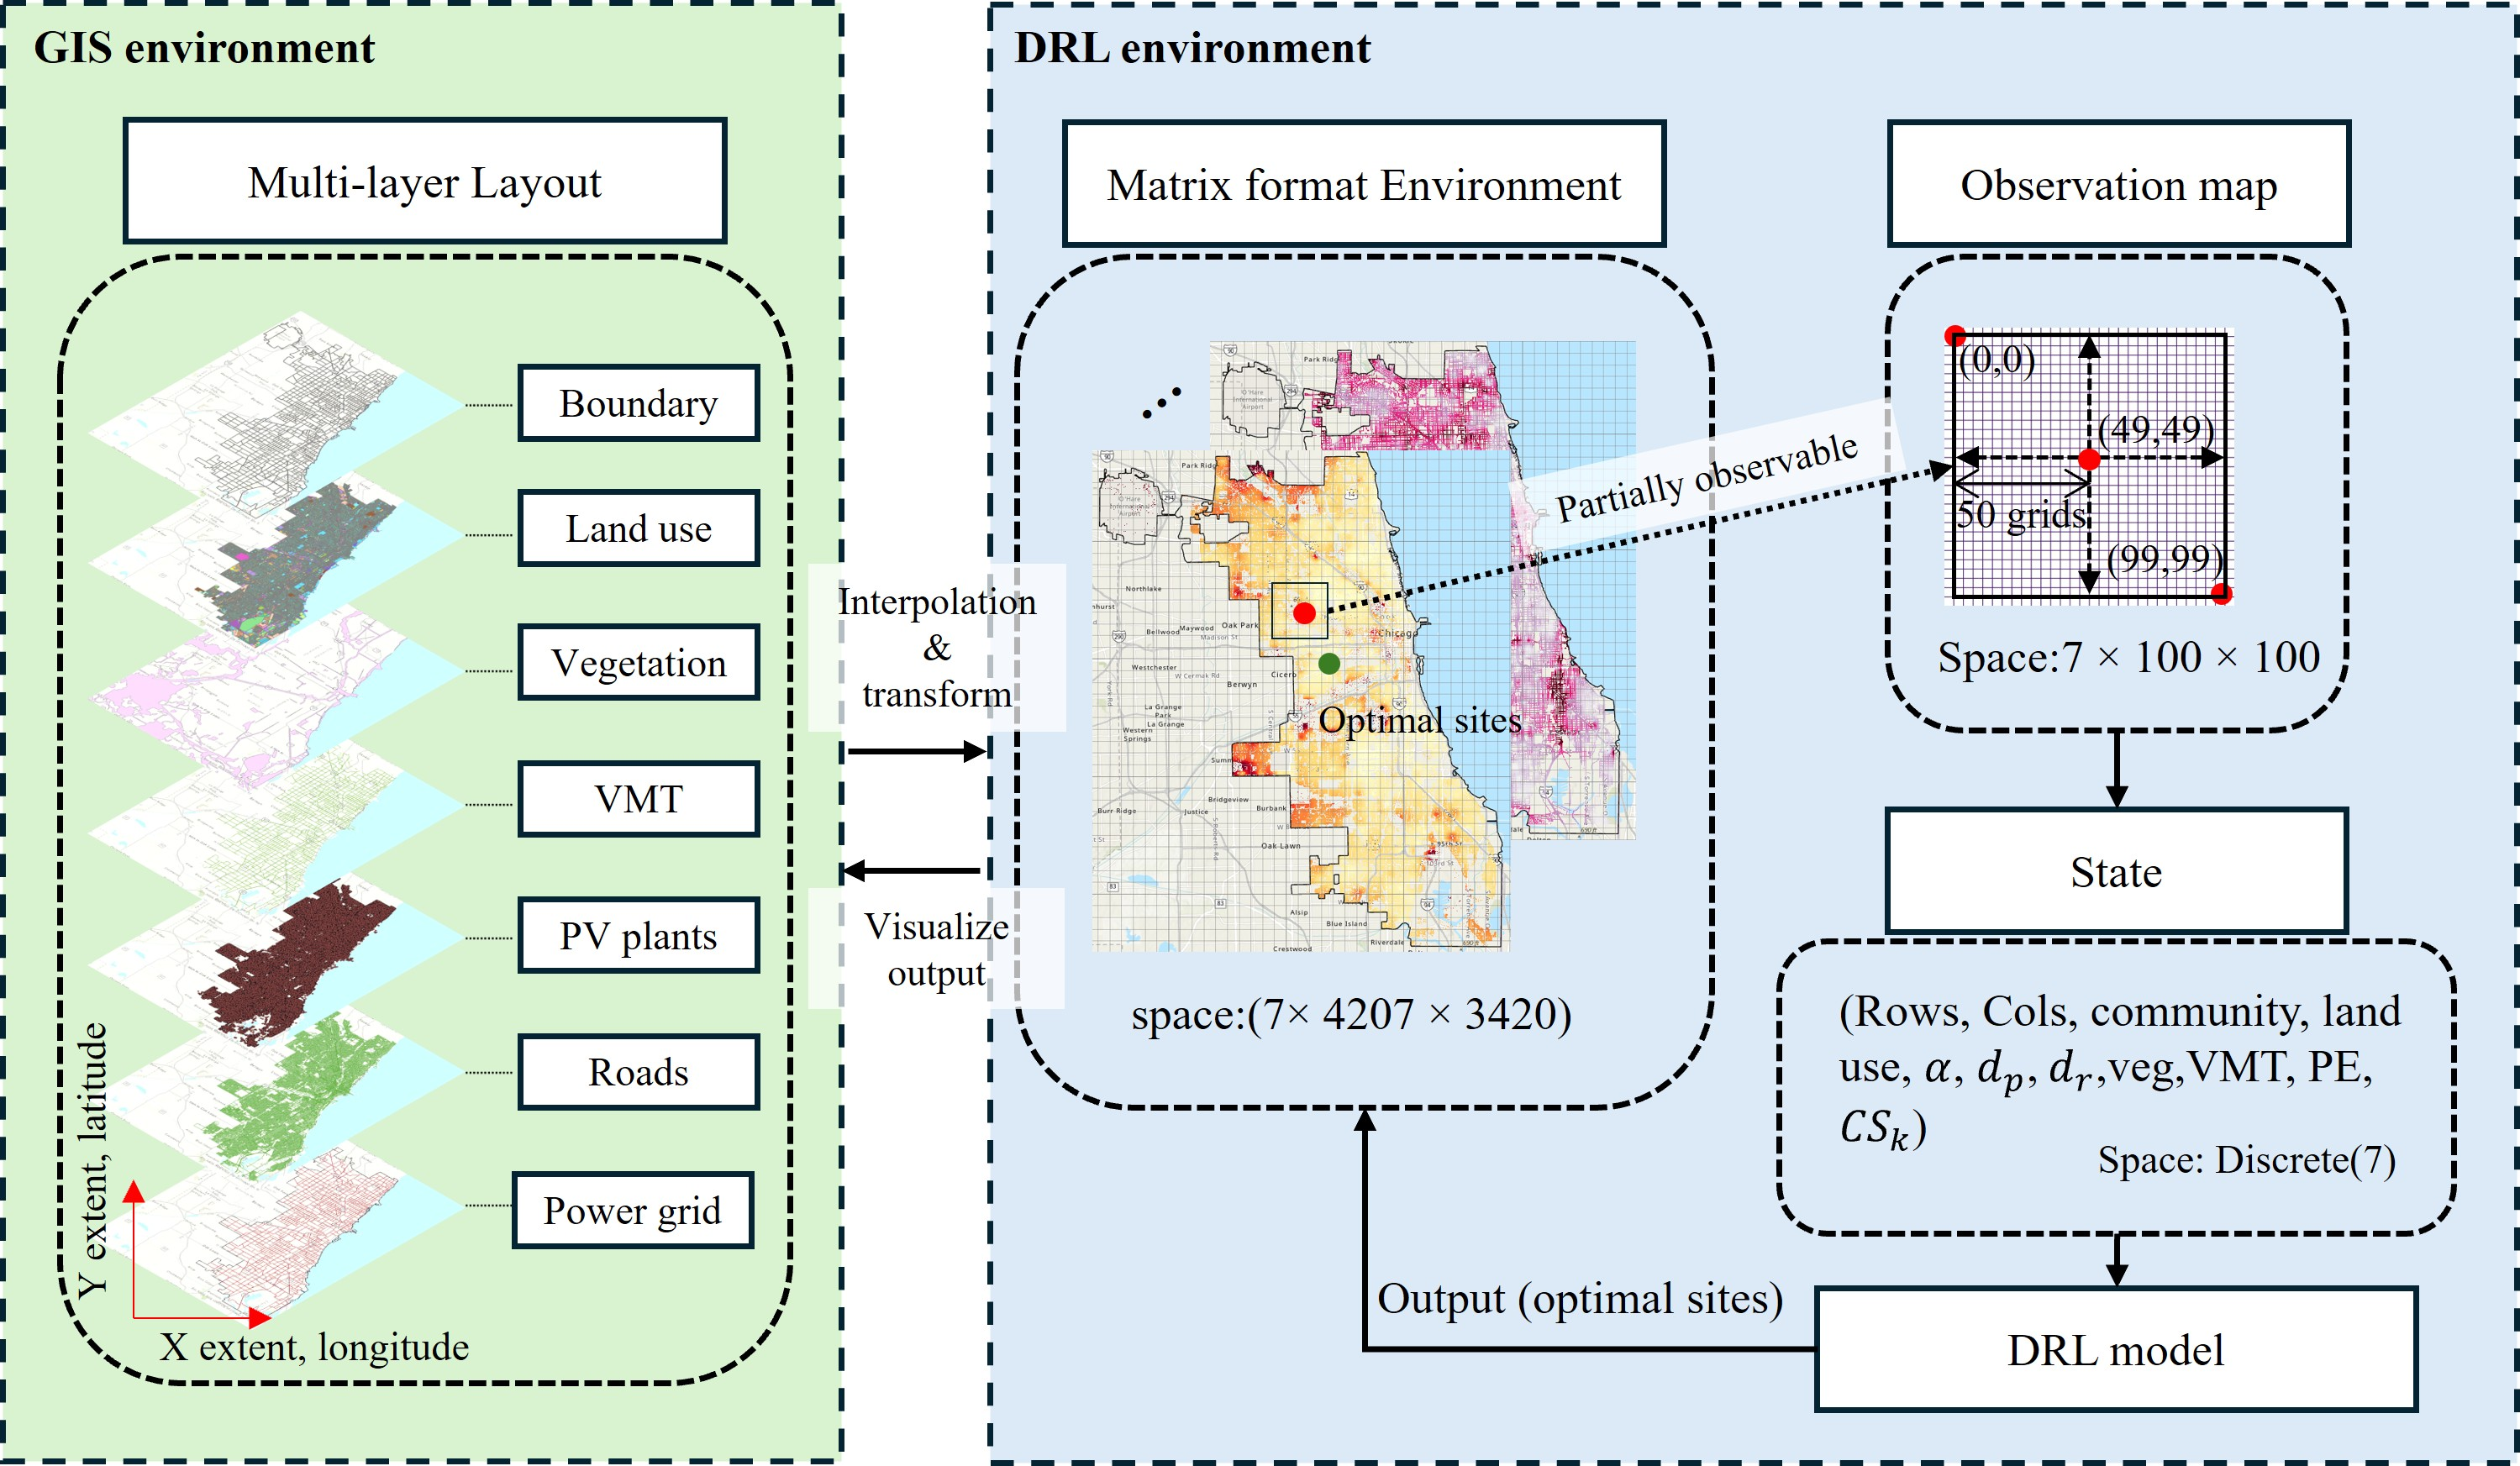
\includegraphics[width=0.8\linewidth]{paper/doc/result_figure/overall environment observation state v4.jpg}
    \caption{Overall progress of input generation and transformation}
    \label{fig:oeos}
\end{figure}
Each grid cell in the environment contains normalized values representing these attributes, allowing the RL agents to make spatially informed decisions.

First, under the environmental criteria, two sub-criteria are considered: vegetation deterioration and expected $CO_2$ emission reduction. The primary objective of the environmental criteria is to minimize environmental degradation through two indicators:
(1) Vegetation deterioration (Erbas et al 2018) \cite{Erbas2018}: This indicator measures the extent of green space disruption caused by land development for EVFCS installation. To ensure practical planning, this study incorporates not only the vegetation level at the candidate site but also the average vegetation density in the surrounding area (i.e., in the observation map). 
(2) $CO_2$ emission reduction (Hosseini and Sarder 2019) \cite{Hosseini2019}: One of the primary motivations for EV adoption is the reduction of GHG emissions during the vehicle use phase. While EVs emit significantly less $CO_2$ compared to internal combustion engine (ICE) vehicles, they are not entirely emission-free due to the fossil fuel-based electricity mix. Therefore, this study considers both (\romannum{1}) the emissions saved from replacing ICE vehicles with EVs and (\romannum{2}) additional reductions achieved through the integration of renewable energy sources, specifically, rooftop solar installations on all buildings in Chicago. It is assumed that all generated solar power is transmitted to nearby EVFCSs to supplement the grid supply. 

Second, under the economic criteria, this study evaluates the investment payback period (Kaya et al. 2022) \cite{kaya_alemdar2022} with the primary objective being to maximize profitability, ensuring that total revenue exceeds total cost. 
(3) Payback period: This is calculated by accounting for the initial capital cost, annual operation and maintenance (O\&M) expenses, and expected revenue from EVFCS operations (Ghosh et al. 2021) \cite{Ghosh2021}. 

Third, the urbanity criteria aim to maximize urban quality by evaluating spatial, infrastructural, and social factors through three sub-criteria.
(4) Harmonization of EVFCS with the roads and power infrastructure (Hisoglu et al 2023) \cite{Hisoglu2023}: This criterion assesses the proximity and accessibility of potential EVFCS locations to roads and the electrical distribution network. The model assumes that CSs prioritize the use of solar-generated electricity, drawing additional power from the grid when necessary. 
(5) Service capability (Kaya et al. 2021) \cite{Kaya_Alem2021}: This indicator evaluates whether the predicted daily charging volume at each site can adequately meet local charging demand, ensuring efficient and equitable service provision.
(6) land use and boundary constraints (Bi et al. 2025) \cite{Bi2025}: This criterion filters out land parcels that are unsuitable for EVFCS installation, including those classified as agricultural, institutional, residential, government-restricted, or miscellaneous zones, based on land use maps. Additionally, areas outside the defined planning boundaries are excluded to ensure that EVFCS installations are confined to viable regions within the designated study area. 

\subsubsection{Agent and action}
This study employs a MORL algorithm in which an agent is assigned to explore the optimal placement of EVFCS based on distinct objectives (e.g., environmental, economic, and urbanity). Agents operate within a shared action space, performing three continuous actions that modify the row, column, and capacity parameters of the EVFCS. The policy learned by the agent outputs normalized actions within the range of [-1, +1] to facilitate stable training. These normalized values are then inverse-transformed to a range of [-50,+50] for the spatial (row and column) actions, which allows the agent to investigate across the grid environment toward optimal sites in subsequent time steps. In addition, the capacity of each charging station is determined by balancing energy supply with charging demand, minimizing $CO_2$ emissions, and incorporating installation cost considerations. The range of capacity values spans from 2 to 14 stalls, corresponding to an energy delivery range of 6 MW/day to 84 MW/day. This is calculated using the transformation function:
\begin{equation}
    6,000 * (\mathrm{action[2] * (\mathrm{max \: capacity} - \mathrm{min \: capacity})/2 + (\mathrm{max \: capacity} + \mathrm{min \: capacity})/2)}
\end{equation} where action[2] is the normalized action from the policy (ranging from -1 to 1), and the minimum and maximum capacity values are set to 2 and 14, respectively, based on historical statistic of the average number of fast charging stalls per station in Chicago (DOE) \cite{DOE_EVCSL}. All charging stalls are assumed to be Tesla V2 Superchargers, each capable of delivering 250 kWh per hour, equivalent to 6 MW/day per stall. Thus, a station with 14 stalls can provide up to 84 MW/day of charging capacity. 

\subsubsection{Observation and state}
Traditional RL typically assumes a fully observable environment, in which the agent has complete access to track the entire state space and learn an optimal policy. It is often impractical in real-world applications, especially in complex, large-scale environments, due to high computational costs and poor generalizability to unseen data. To effectively explore large and complex urban environments, this study adopts a partially observable environment, where the agent receives partial information about the environment at a specific location. The observation is defined as a localized window of the environment map that contains critical geospatial information, as shown in \textcolor{red}{Figure} \ref{fig:oeos}, allowing the agent to make informed decisions at each step. Each observation is structured as a 7 (e.g., multi-layers) $\times $ 100 $\times $ 100 grid (e.g., 1 grid = 100 meters), centered around the agent's current position. In other words, the agent is placed at the centroid of the observation window, corresponding to grid coordinates (49, 49). For instance, the agent, currently positioned at (1500,1400) in the matrix format environment coordinates, selects an action of (-0.5, +0.5) for the row and column directions, respectively, as output by the DRL policy, these normalized values are transformed into (24, 74) as grid coordinates. As a result, the agent moves to a new position at (1476, 1474) in the matrix format global environment. In contrast to previous work (Heo and Chang 2024), which directly mapped observations to states, this study compresses the high-dimensional observation into a more compact state vector consisting of seven continuous representative features. Given the complexity of the environment map, which overlays seven geospatial data layers, directly using the observation map would substantially increase computational load and degrade model performance due to including the noise. The state includes the following components: Row and column coordinates (agent position), community boundary index, land use classification, the propotion of replacement energy generation with solar potential ($\alpha$), minimum distance to the power grid ($d_p$), minimum distance to the road network ($d_r$), average vegetation canopy coverage  (veg), average vehicle miles traveled (VMT), average potential electricity generation (PE), and average distance to candidate charging stations ($CS_k$) within the observation window, as shown in \textcolor{red}{Figure} \ref{fig:oeos}. This compact representation enables efficient policy learning while retaining the critical spatial and contextual information necessary for optimal decision-making. 

\subsubsection{Reward function}
The reward function is a critical component that directly affects the performance and learning efficiency of RL agents in achieving their defined goals. Specifically, in this study, a MORL framework is employed, wherein agents are assigned an independent objective corresponding to a specific sustainability criterion. Accordingly, each agent is guided by a distinct reward function tailored to its respective goal. The policies learned by the agents are categorized into three main criteria, environmental, economic, and urbanity, which collectively encompass multiple sub-criteria (6). Each agent independently investigates the optimal policy within its designated domain using DRL. For example, the agent assigned to the economic criterion aims to maximize profitability by optimizing the trade-off between the sizing of CSs, corresponding to the total costs and operational revenues.

In the environmental criteria, $R_1$ aims to maximize the preservation of vegetation during a charging station installation (i.e., minimization of vegetation deterioration) and to enhance the reduction of $CO_2$ emissions associated with both travel and energy generation corresponding to charging demand. Specifically, the vegetation preservation is evaluated using two sub-criteria: (1) the average vegetation ratio in the observation map ($r_{avm}$), and 2) vegetation canopy density at the agent's location ($r_{viss}$). To maximize environmental prevention, the agent is incentivized to avoid areas with high vegetation density when selecting EVFCS installation sites. For example, when the agent is positioned in a location where the average vegetation ratio ($avm$) is 0.40 and the local canopy ratio ($viss$) is 0.50, the combined vegetation preservation score is computed as:
\begin{equation} \label{eq-b}
    r_{avm}+r_{viss}=e^{-avm} + e^{-viss}
\end{equation}
In this example, the total environmental preservation score equals approximately 1.28, indicating the environmental cost of siting in a moderately vegetated area. Higher scores are achieved by selecting areas with minimal vegetation, aligning with the sustainability objective of minimizing environmental impact. Furthermore, the total reduction in $CO_2$ emissions ($r_{TER}$) achieved by EVs is calculated by considering the emissions avoided during vehicle operation and those reduced through the integration of alternative energy sources. Specifically, $r_{TER}$ is derived from the combined effect of two components: (1) the reduction of $CO_2$ emissions due to replacing ICE vehicles with EVs while driving ($r_{apr}$) and (2) the additional reduction from substituting fossil fuel-based electricity with solar power ($r_{eser}$). The avoided emissions from EV driving, $r_{apr}$, are calculated based on average fuel consumption and emission rates of ICE vehicles:
\begin{equation} \label{eq-c}
    r_{apr}=\mathrm{VMT} * \frac{23.7 (\mathrm{lbs.CO_2e/1gal})}{21.79 (\mathrm{mi/1gal}))}
\end{equation}
The emissions reduced from electricity substitution, $r_{eser}$, are calculated as:
\begin{equation} \label{eq-d}
    r_{eser}=(1-\alpha)*\mathrm{VMT} * 0.72576 / 4.56
\end{equation}
where $\mathrm{VMT}$ refers to vehicle miles traveled, indicating the total number of miles driven by EVs within a one-mile unit of road. The parameter $\alpha$ denotes the proportion of electricity replaced with solar power generation. This study assumes that all EVs are Tesla Model 3 vehicles, with an efficiency of 4.56 mi/kWh. The average $CO_2$ emission factor for electricity generation in Illinois is set as $0.72576 \: \mathrm{lbs. \: CO_2e/kWh}$. The probability of visiting a CS is based on a traffic flow-adjusted value of 1.064\%, reflecting the national market share of light-duty EVs in the United States. The combined effect is scaled using the logistic function shown in Equation \eqref{eq-e}.
\begin{equation} \label{eq-e}
    r_{TER} = 1-e^{-(r_{apr}+r_{eser})*0.01064}
\end{equation}
To align the scale of $r_{TER}$ with that of the vegetation preservation sub-criteria ($r_{avm}$), the total $CO_2$ reduction score is rescaled using the exponential transformation $1-e^{-r_{TER}}$. The final environmental reward $R_1$ is computed as a weighted average of the two vegetation-related sub-criteria and the total $CO_2$ reduction:
\begin{equation} \label{eq-a}
    R_1=0.3*r_{avm}+0.3*r_{viss}+0.4*r_{TER}
\end{equation}

In the economic criteria, $R_2$ evaluates the financial feasibility of EVFCS deployment by maximizing profitability while balancing station capacity with local charging demand. Specifically, $R_2$ is designed to optimize the payback period by calculating the profitability of each charging station and comparing it against installation and operational costs. The goal is to achieve cost recovery within an expected payback period of 12 years. The yearly profitability of a charging station, denoted as $P_G$, is derived from revenue generated through charging, as defined in Equation \eqref{eq-f}.
\begin{equation} \label{eq-f}
   \mathrm{payback \: period} (R_2)= \frac{F *12 \mathrm{years}}{ P_G*(\alpha*(0.28-0.06) + (1-\alpha)*(0.28-0.0405)) * VMT * 365}
\end{equation}
This equation accounts for the profit margin from selling electricity via Tesla Superchargers (at an average rate of \$0.28/kWh), relative to the costs of supplying energy from two sources: alternative (solar) energy (\$0.06/kWh) and commercial grid electricity (\$0.0405/kWh in Chicago). The weighted combination is determined by $\alpha$. The installation and operational cost of a charging station, denoted $F = z *(20,600*0.2+800)$, consists of the cost of fast-charging stalls and maintenance expenses. The average installation cost per stall is \$20,600 (150kW), with up to 80\% covered by incentives. Annual maintenance is represented by a coefficient $\rho$ of \$800 per charger. Also, $z$ is the number of stalls at the charging station. The reward function $R_2$ provides a positive reward of +12 if the probability of the station exceeds the total cost within the expected 12-year payback period, reinforcing cost-efficient allocation decisions in the DRL framework. 

In the urbanity criteria, $R_3$ assesses the overall usability and practicality of EVFCSs deployment in the target urban area. As defined in Equation \eqref{eq-g}, $R_3$ returns a positive reward (+12) when four key sub-criteria are met: (1) feasibility of construction of the EVFCS ($r\_drn$), (2) accessibility to roads ($r\_dg$), (3) proximity to electrical distribution network or solar panels installed in building rooftops ($r\_lu$), and (4) affordability of charging demand based on station capacity ($r\_sc$). 
\begin{equation} \label{eq-g}
    R_3 = \frac{(r_{drn}+r_{dg} + r_{lu} + r_{sc})}{4}*12
\end{equation}
Each sub-criterion contributes to evaluating the site's suitability for EVFCS implementation. For instance, construction feasibility $r\_drn$ penalizes placements in areas where EVFCS installation is restricted, such as residential, institutional, government-restricted, miscellaneous land zones, or out of boundaries. In such cases, $r_drn$ receives a penalty score of 0. Road accessibility $r_{dg}$ captures the agent's proximity to road networks, calculated via the Euclidean distance from the agent's position to the nearest road. If the agent is within a 500m radius, $r_{dg}$ receives a reward of +1. Electricity supply access $r_{lu}$ evaluates the availability of nearby distribution networks or rooftop solar power installations. The reward varies based on the solar power substitution ratio ($\alpha$): +1 for fully supplied charging demand $\alpha = 1$, +0.5 for partial supply ($0 < \alpha <1$) with capable of accessibility to power grids (agent's proximity to grid is within 500m), and 0 for no accessible solar generation ($\alpha=0$). Charging demand affordability $r_{sc}$ checks whether the predicted capacity of the charging station (based on the agent's selected action) meets the local charging demand. If the predicted capacity exceeds the estimated demand ($\mathrm{VMT}/4.56$ MW), $r_{sc}$ is assigned a reward of +1. The urbanity criteria encourage the agent to choose locations that are feasible, accessible, well-connected to the energy grid or renewable sources, and adequately sized to meet local charging demand. 

\subsubsection{Policy Gradient Method}
The policy gradient method is a foundational approach in RL that seeks to directly model and optimize the policy to achieve the agent's goal of maximizing expected discounted rewards. Instead of learning a value function, policy gradient methods optimize a parameterized policy $\pi_\theta(a|s)$ by adjusting the policy parameters $\theta$ in the direction that increases expected performance. The objective is to find the optimal policy by maximizing the scalar performance measure $\nabla _{\theta}J(\theta)= \sum_{s}^{}\nabla_\theta\log\pi_\theta(a|s)R(\tau)$, where $R(\tau)$ denotes the cumulative reward (return) over trajectory $\tau$, and $\nabla_\theta\log\pi_\theta(a|s)\cdot R(\tau)$. indicates the direction in which the probability of selecting an action in stat increases most rapidly. Intuitively, this gradient encourages the policy to increase the likelihood of action-state pairs $(s_t,a_t)$ that yield high returns. For example, if the return associated with a given trajectory is high, the network increases the probability of selecting the corresponding action in the same state in future iterations. However, a major challenge of this method is its high variance, as updates rely heavily on individual trajectory samples and lack a true baseline for estimating return. As a result, different trajectories originating from the same state can yield varying returns, which may destabilize learning and slow convergence. 

The actor-critic method is a widely used RL framework that simultaneously learns both policy (the actor) and a value function (the critic). The actor-critic architecture enables the policy to be updated based on value-based feedback, offering improved stability and sample efficiency compared to pure policy gradient methods. In this method, the actor refers to the learned policy $\pi_\theta(a|s)$, which determines the action to take in a given state and is updated in the direction suggested by the critic. The critic estimates the value function, which provides a baseline for evaluating how good an action is in a specific state. The advantage actor critic (A2C) algorithm enhances this method by updating policy parameters using the advantage function ($A(s,a)$), which compares the estimated future reward for taking action in state to the average value of the same state $V(s)$. The advantage is defined as $A(s,a)=Q(s,a) - V(s)=r+\gamma V(s')-V(s)$. If $A(s,a) > 0$, the agent receives positive feedback, and the gradient is updated in a direction that increases the probability of selecting action in state. By incorporating advantages, A2C reduces the variance of the policy gradient, stabilizing training while maintaining learning effectiveness. For environments requiring continuous actions, actions are sampled from a Beta distribution parameterized by the policy network. The policy is represented as: 
\begin{equation}
    f(x;\alpha,\beta)=\frac{\Gamma(\alpha+\beta)}{\Gamma(\alpha)\Gamma(\beta)}x^{\alpha-1}(1-x)^{\beta-1}
\end{equation}
where $\alpha$ and $\beta$ denote the shape parameters and $\Gamma(\cdot)$ denotes the Gamma function that extends factorial to real numbers. The beta distribution can reduce the bias bound of the action space, as the Gaussian distribution does (Chou et al. 2017) \cite{Chou2017}. This probabilistic formulation enables a balance between exploration and exploitation. In this study, three continuous actions are sampled from the Beta distribution policy, where the action outputs are constrained to the range [0,1]. 

One of the main challenges of the A2C algorithm is its tendency to update the policy aggressively after every step, without applying thresholds or constraints to the model parameters. This can lead to instability in training, such as vanishing or exploding gradients, and poor sample efficiency, ultimately resulting in convergence issues.

To address the instability and inefficiency challenges in policy gradient optimization, proximal policy optimization (PPO) has been proposed as a more stable and sample-efficient alternative. PPO is to compute a clipped surrogate objective that on the probability ratio ($r_t(\theta)$) between the current and old policies $r_t(\theta)=\frac{\pi_\theta(a_t|s_t)}{\pi_{\mathrm{old}}(a_t|s_t)}$ that measures how does the likelihood of selecting action under the new policy compares to that under the old policy. Rather than allowing large destabilizing policy updates, PPO constraints policy updates using a clipping mechanism, which limits how far the $r_t(\theta)$ can deviate from 1 (ie., trust region):
\begin{equation}
    L^{\mathrm{CLIP}}(\theta)=\mathbb{E}[\mathrm{min}(r_t(\theta)\hat{A_t}, \mathrm{clip}(r_t(\theta)_,1-\epsilon, 1+\epsilon)\hat{A_t})]
\end{equation}
Here, $\hat{A_t}$ denotes the estimated advantage function, and $\epsilon$ denotes a small positive constant that defines the allowable range of change in the policy. The use of the clip function ensures that the objective is clipped to prevent excessive updates if the $r_t(\theta)$ exceeds the trust region. This conservative update strategy improves training stability, enhances sample efficiency, and mitigates the risk of policy collapse.

To investigate optimal places of EVFCS placement sites that satisfy multiple objectives, this study implements two learning algorithms: (1) a single-policy-based multi-objective reinforcement learning (MORL) approach and (2) a multiple-policy-based asynchronous federated reinforcement learning approach. The MORL approach seeks to learn a policy that balances trade-offs among distinct objectives, environmental, economic, and urbanity.

Single-policy MORL algorithms employ a linear scalarization function to combine multiple objectives into a single policy. This is achieved by computing a weighted sum of the $\hat{Q}$-vector and a non-negative weight vector:
\begin{equation}
    \hat{SQ}_{linear}(s,a) =\sum_{o=1}^{m}\mathrm{w}_o\cdot\hat{Q}_o(s,a) \quad \text{where } \sum_{i=1}^{n} \mathrm{w}_o = 1, \quad w_o \geq 0
\end{equation}
where $\hat{Q}$-vector denotes the estimated action-value function for objective $o$, and $w_o$ denotes the weight assgined to that objective. The $\hat{Q}$ vector is computed based on the policy $\pi_\theta(a|s)$ parameterized by $\theta$, and multiple reward signals $R_t^{(i)}$, each corresponding to a distinct objective $i \in {1,2,3}$ (de Oliveira et al. 2021) \cite{Oliveira2021}, as illustrated in \textcolor{red}{Figure} \ref{fig:aospmorl}. 

\begin{figure}[h]
    \centering
    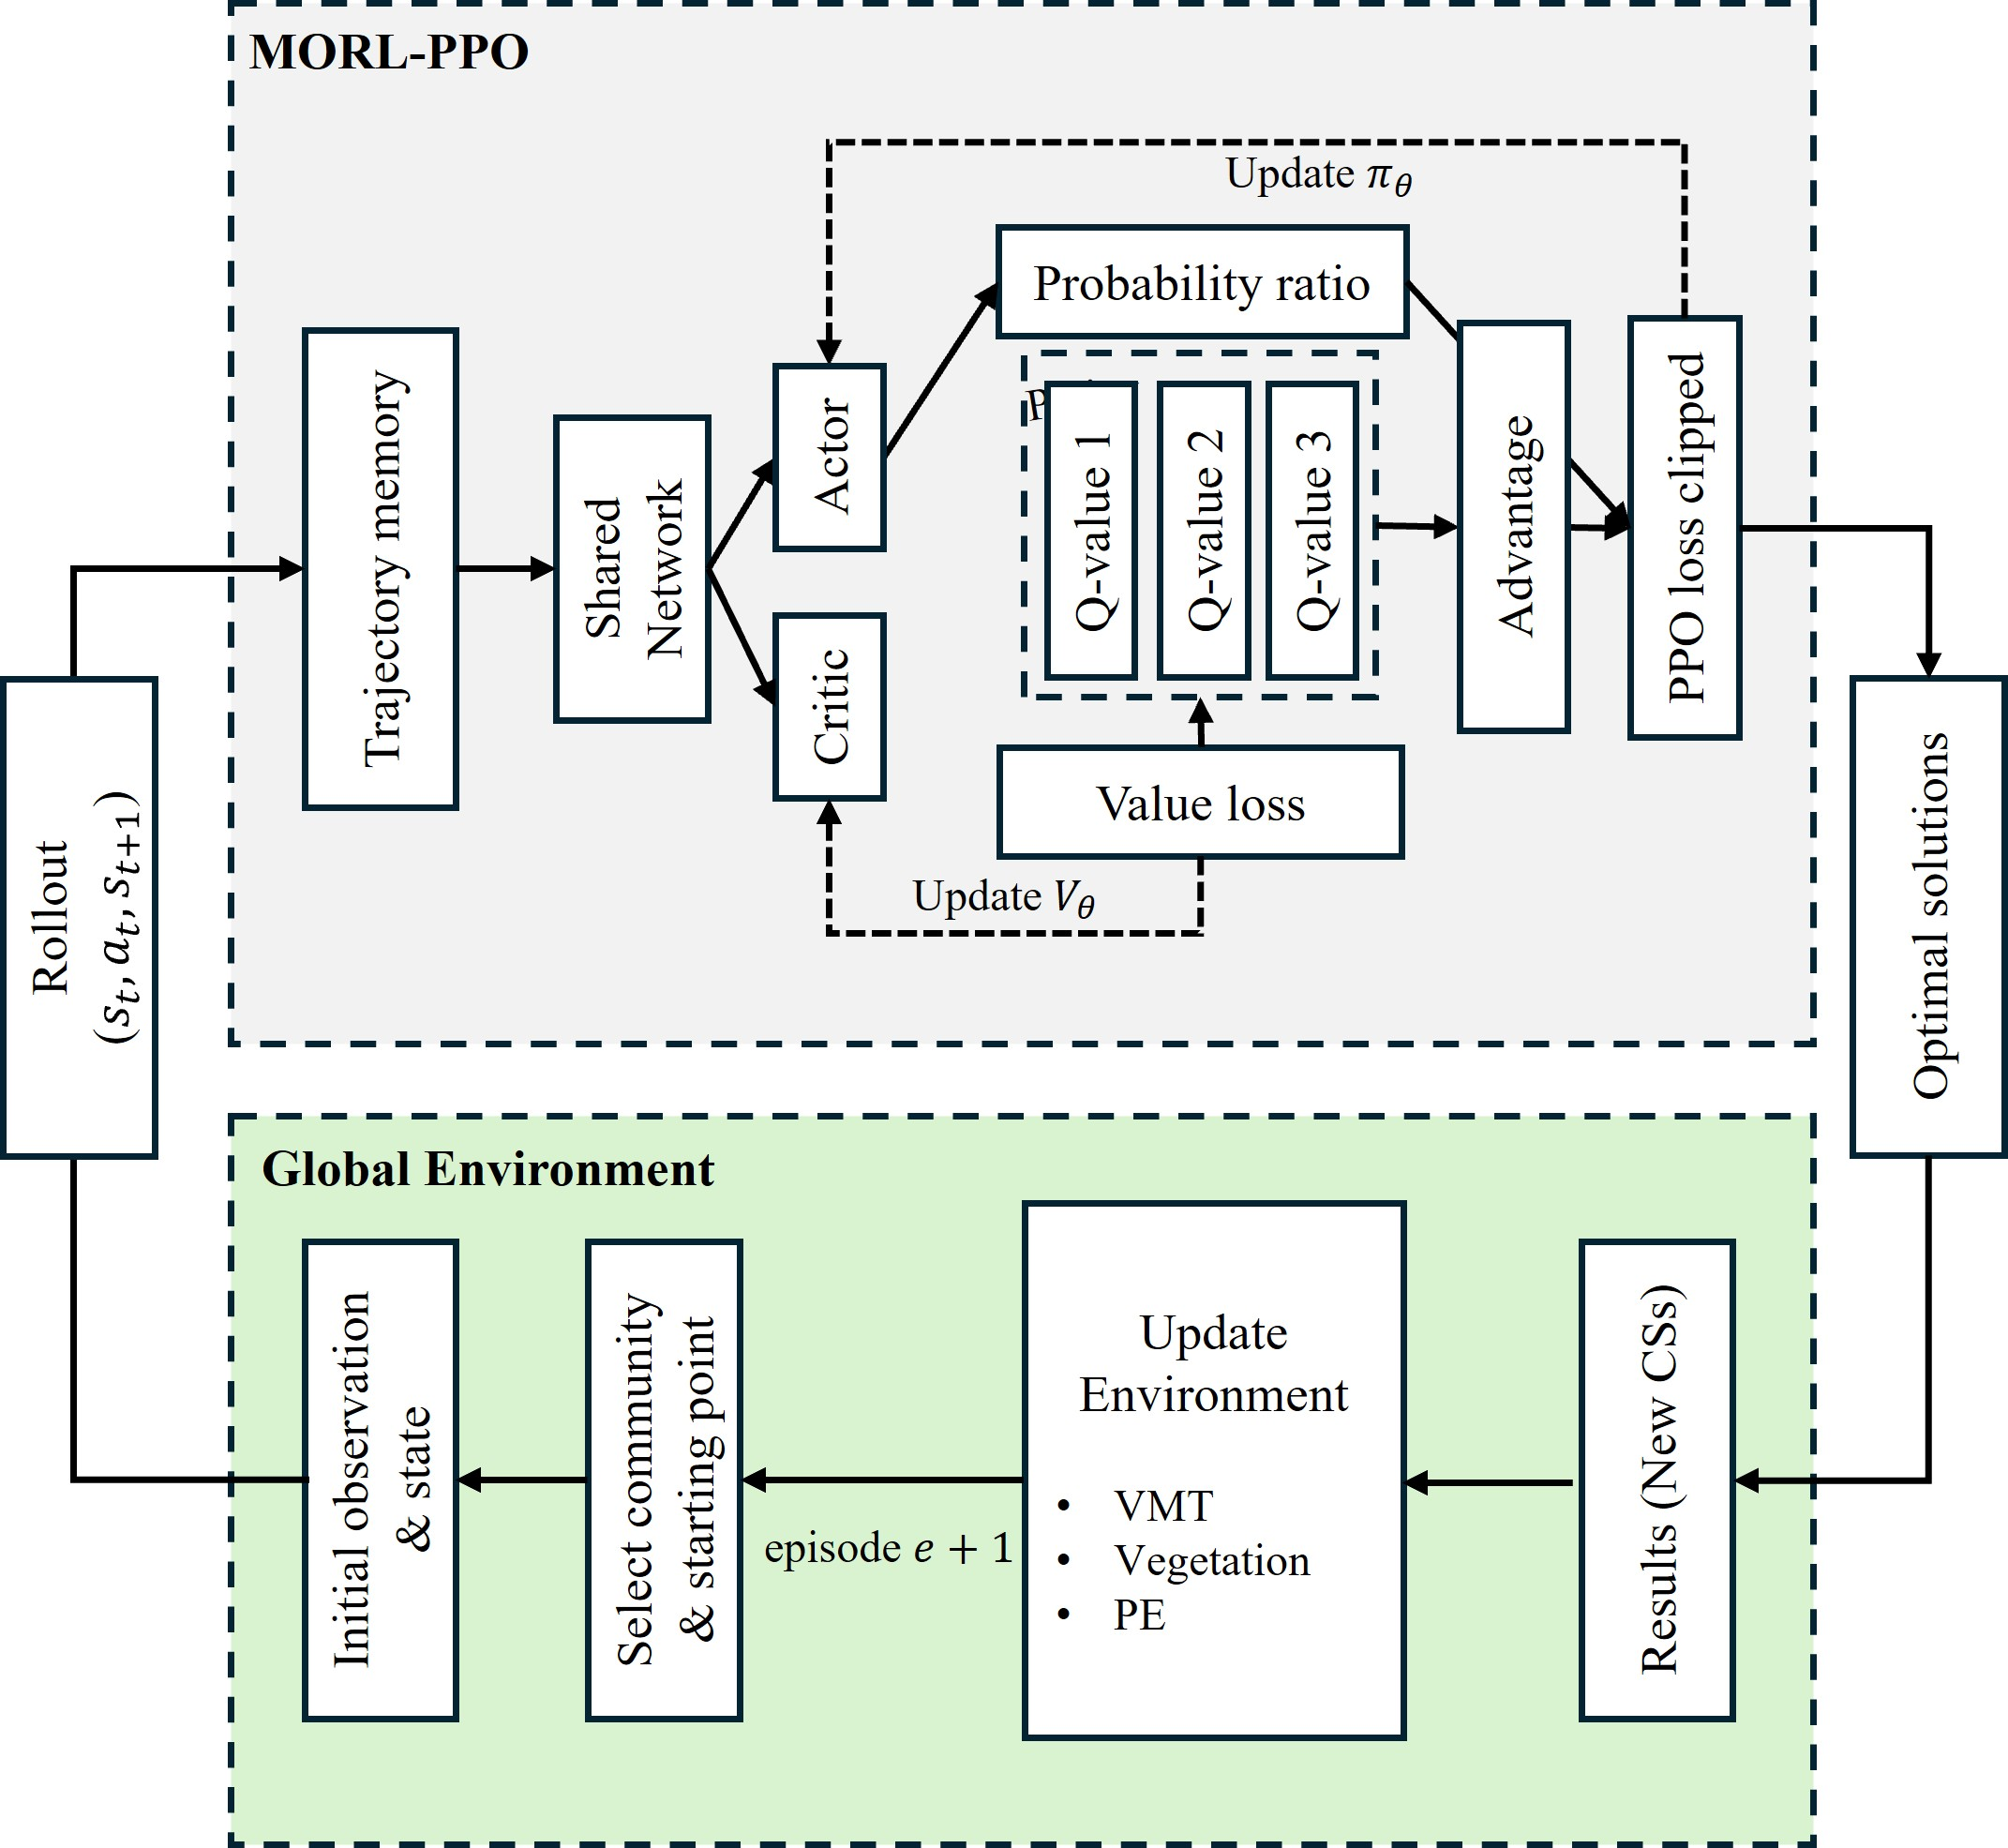
\includegraphics[width=0.7\linewidth]{paper/doc/result_figure/MORL PPO_v2.jpg}
    \caption{Architecture of single policy MORL}
    \label{fig:aospmorl}
\end{figure}
In this study, the reward weights are assigned as follows: 0.3 for the environmental objective, 0.4 for the economic objective, and 0.3 for the urbanity objective. This convex combination forms the total reward, which is then used to compute the advantage function for policy gradient optimization.

To extend the probability ratio to the multi-objective setting, the value loss for each objective $i$ is defined as:
\begin{equation}
    L^{VF}_i(\theta) = \left( V_\theta^{(i)}(s_t) - R_t^{(i)} \right)^2
\end{equation}
The final multi-objective PPO loss becomes:
\begin{equation}
    \underset{\theta}{\text{maximize}} \quad 
    \mathbb{E}_t \left[
L^{CLIP}(\theta)
- \sum_{i=1}^{n} c_{v}^{(i)} L^{VF}_i(\theta)
+ c_e S[\pi_\theta](s_t)
\right]
\end{equation}
where $c_v^{(i)}$ denotes the value loss coefficient for each objective $i$, $S[\pi_\theta](s_t)$ denotes entropy regularization, and $c_e$ is the entropy regularization coefficient.

On the other hand, the multi-policy-based asynchronous federated MORL algorithm aggregates three predefined local policies to update a shared global policy (Hayes et al 2022) \cite{Hayes2022}, as illustrated in \textcolor{red}{Figure} \ref{fig:aoampfmoo}.

\begin{figure}[h]
    \centering
    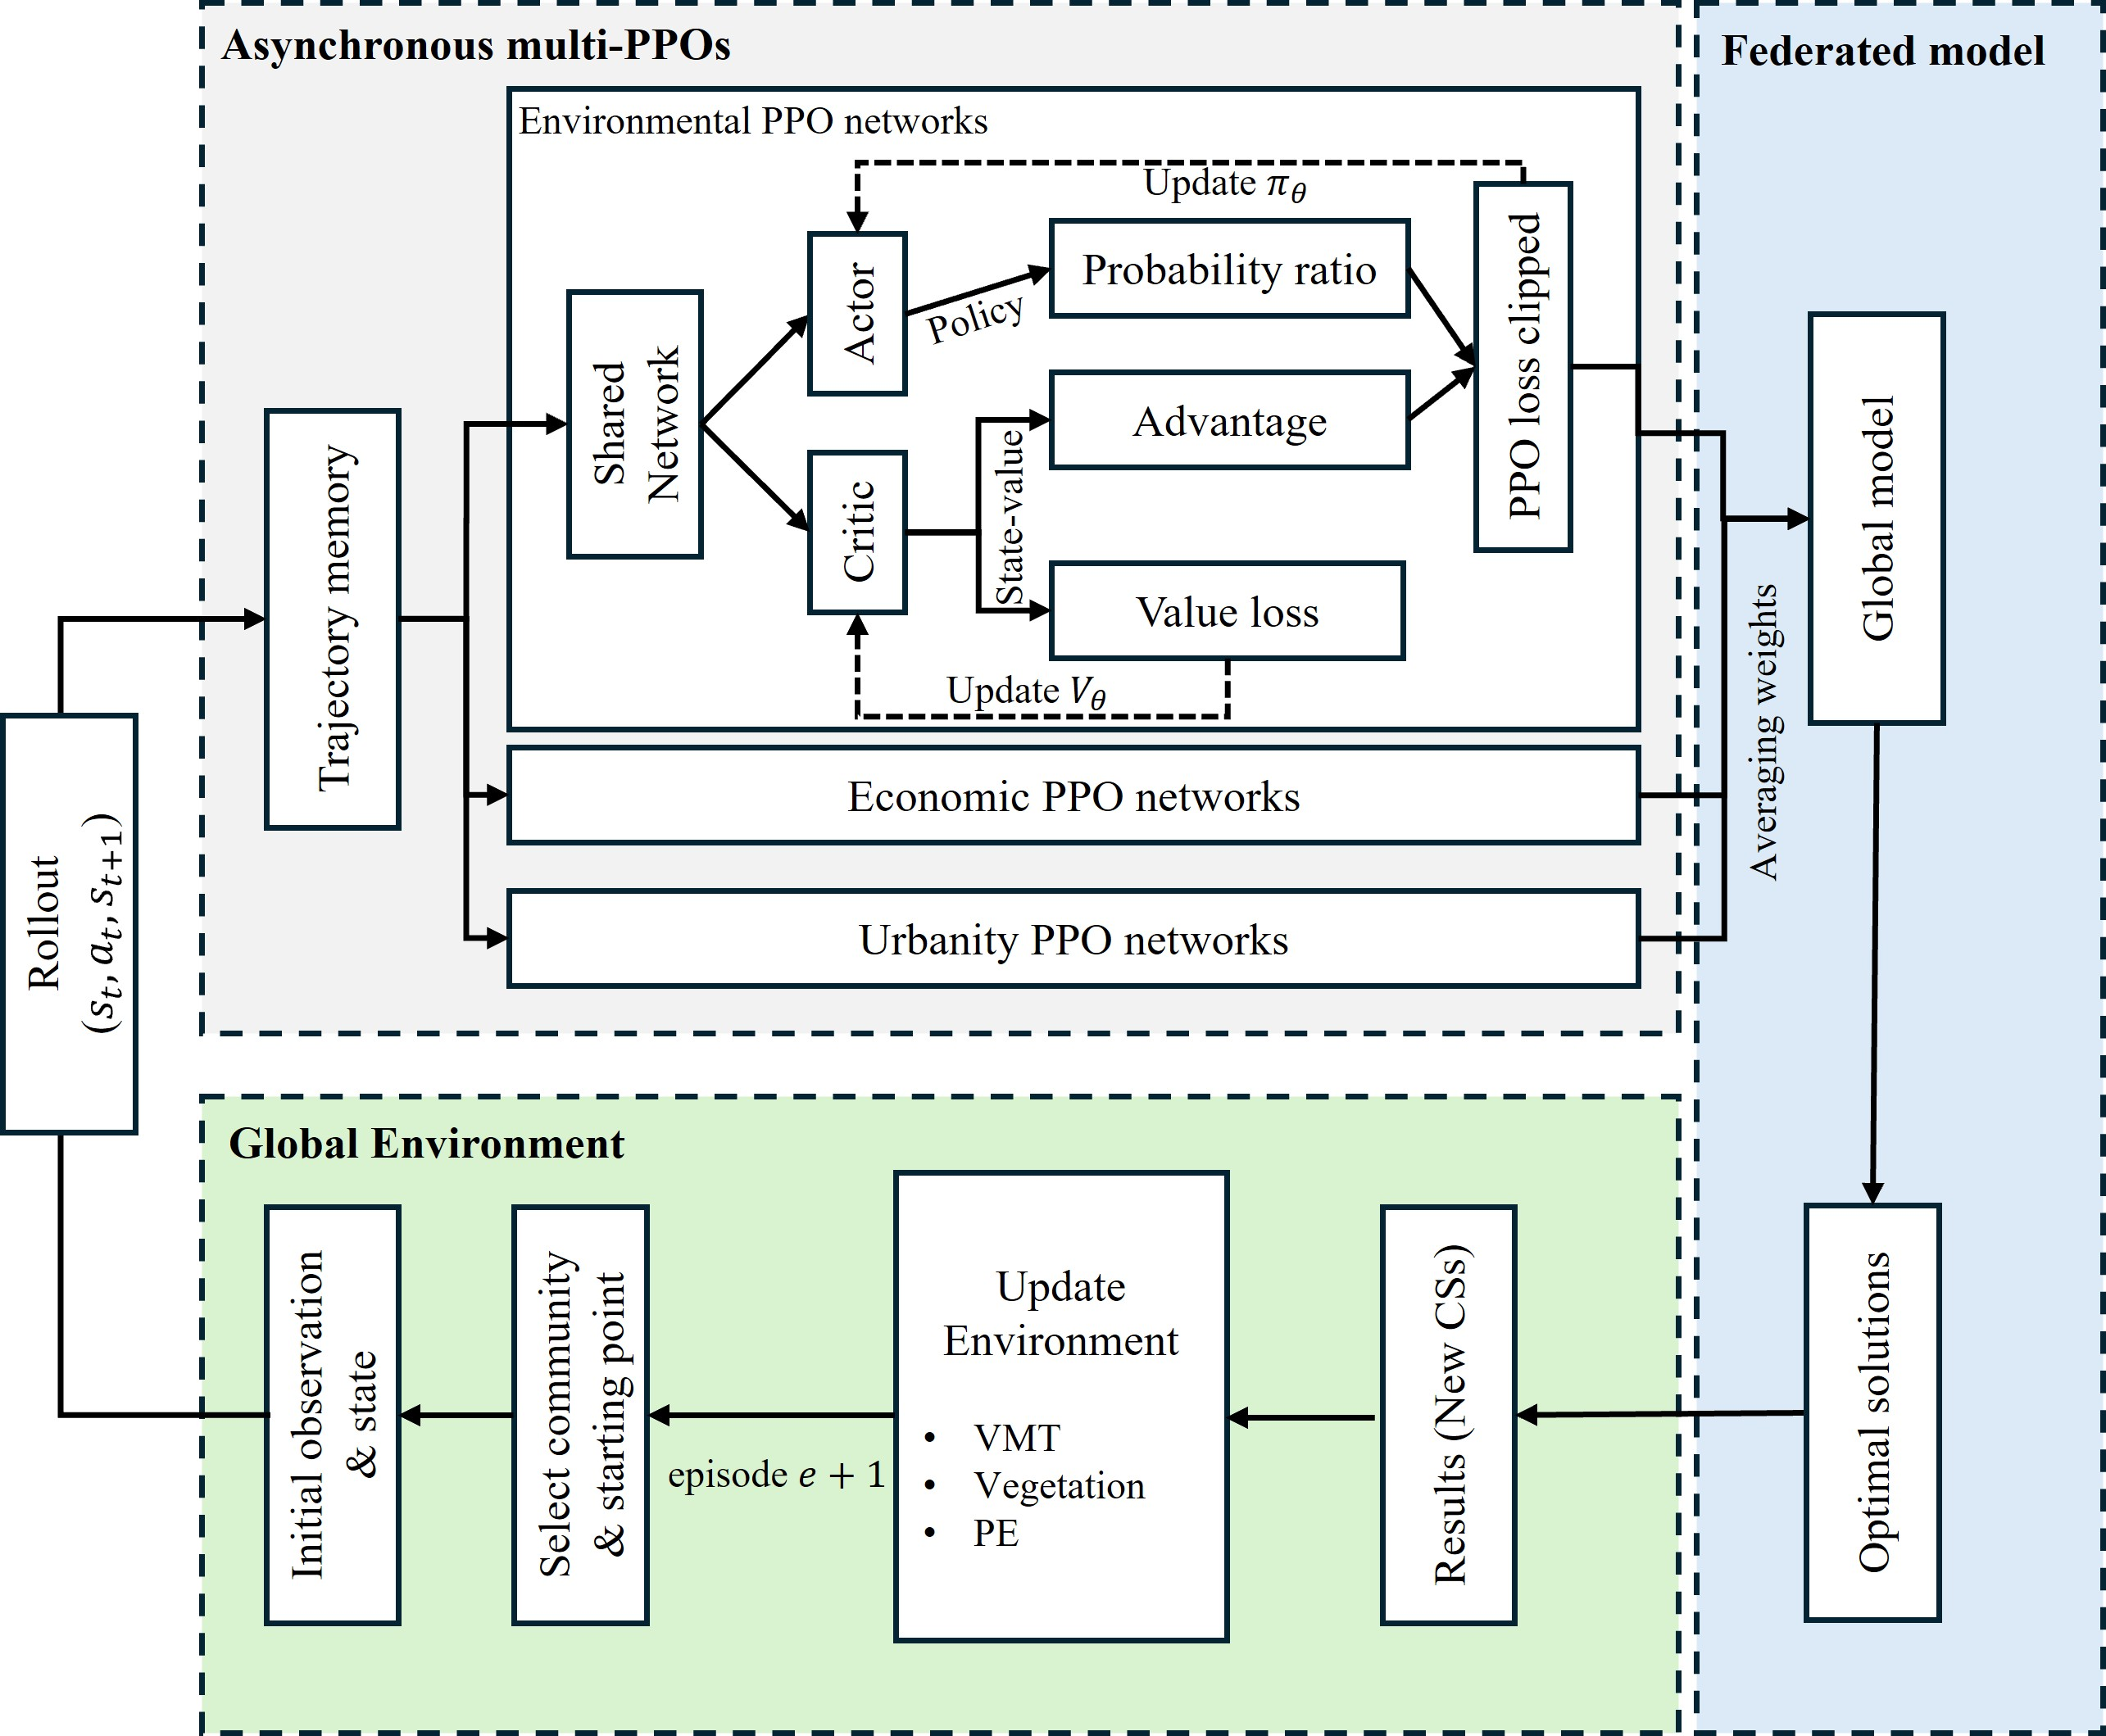
\includegraphics[width=0.7\linewidth]{paper/doc/result_figure/asynchronous multi PPOs_v2.jpg}
    \caption{Architecture of asynchronous multi PPOs for multi-objective optimization}
    \label{fig:aoampfmoo}
\end{figure}
In this algorithm, each agent independently solves its own PPO optimization problem:
\begin{equation}
    \underset{\theta^{(m)}}{\text{maximize}} \quad 
\mathbb{E}_t^{(m)} \left[
L^{\text{CLIP}}(\theta^{(m)})
- c_v^{(m)} L^{\text{VF}}(\theta^{(m)})
+ c_e^{(m)} S[\pi_{\theta^{(m)}}]
\right]
\end{equation}
Each agent trains its policy using only local data $\mathcal{D}^{(m)}$, without sharing raw trajectories or rewards. This decentralized approach respects privacy constraints and enables scalable, parallelized learning across agents. Once the local policies are updated, the global policy is computed via federated averaging, which combines model parameters based on the relative data size $n_m$ from each agent:
\begin{equation}
    \theta^{(\text{global})}_{t+1} = \sum_{m=1}^{M} \frac{n_m}{\sum_{j=1}^{M} n_j} \theta^{(m)}_t
\end{equation}
This federated approach ensures that the global model evolves by incorporating diverse perspectives from multiple objectives.

\subsubsection{Overall decision-making strategy in the MODRL}
This study investigates the optimal allocation of EVFCSs over episodes, where each episode represents a potential deployment instance (i.e., placement of a charging station) in a large-scale environment. Unlike traditional RL settings that reset the environment at the beginning of each episode, the global environment in this study is dynamic and non-resettable. The environment continuously updates key variables, such as VMT, potential electricity values, potential CS locations, and vegetation canopy, upon each installation of an EVFCS. At the beginning of each episode, a specific community area (among 77 in Chicago) is selected to prevent biased EVFCS deployment across the urban areas. Initially, community selection follows a uniform distribution (i.e., $1/77$) to ensure diverse sampling of potential CS locations. Once an initial sampling threshold (e.g., 100 EVFCSs) is reached, the selection process transitions to a Kernel density-based probability distribution, as shown in Equation \eqref{eq-aa}.
\begin{equation} \label{eq-aa}
    \mathrm{Density}(D)=\frac{1}{r^2_k}\sum_{i=1}^{n}[\frac{1}{\sqrt{2\pi}}*\mathrm{pop}_i*e^{\frac{(\frac{d}{r})^2}{2}}]
\end{equation}
where $r_k$ denotes the radius of community $k$, $\mathrm{pop}_i$ denotes the count of EVFCSs at point $i$ (i.e., charging stations), and $d$ denotes the Euclidean distance between point $i$ and the centroid of community polycon. The Kernel density captures the spatial concentration of installed CSs in the vicinity of each community centroid, with the radius adjusted by the area of the community. The resulting density values are then normalized into a probability distribution using Equation \eqref{eq-bb}:
\begin{equation} \label{eq-bb}
    P_k=\frac{w_k}{\sum_{i=1}^{N}w_i}, \quad w_k=\frac{1} {e^{D}+\epsilon}
\end{equation}
where $N$ denotes the total number of communities (i.e., 77) and $\epsilon$ denotes a small constant to prevent division by zero during normalization. A random starting point is then sampled within the selected community, as illustrated in \textcolor{red}{Figure} \ref{fig:seofsm}.
\begin{figure}[h]
    \centering
    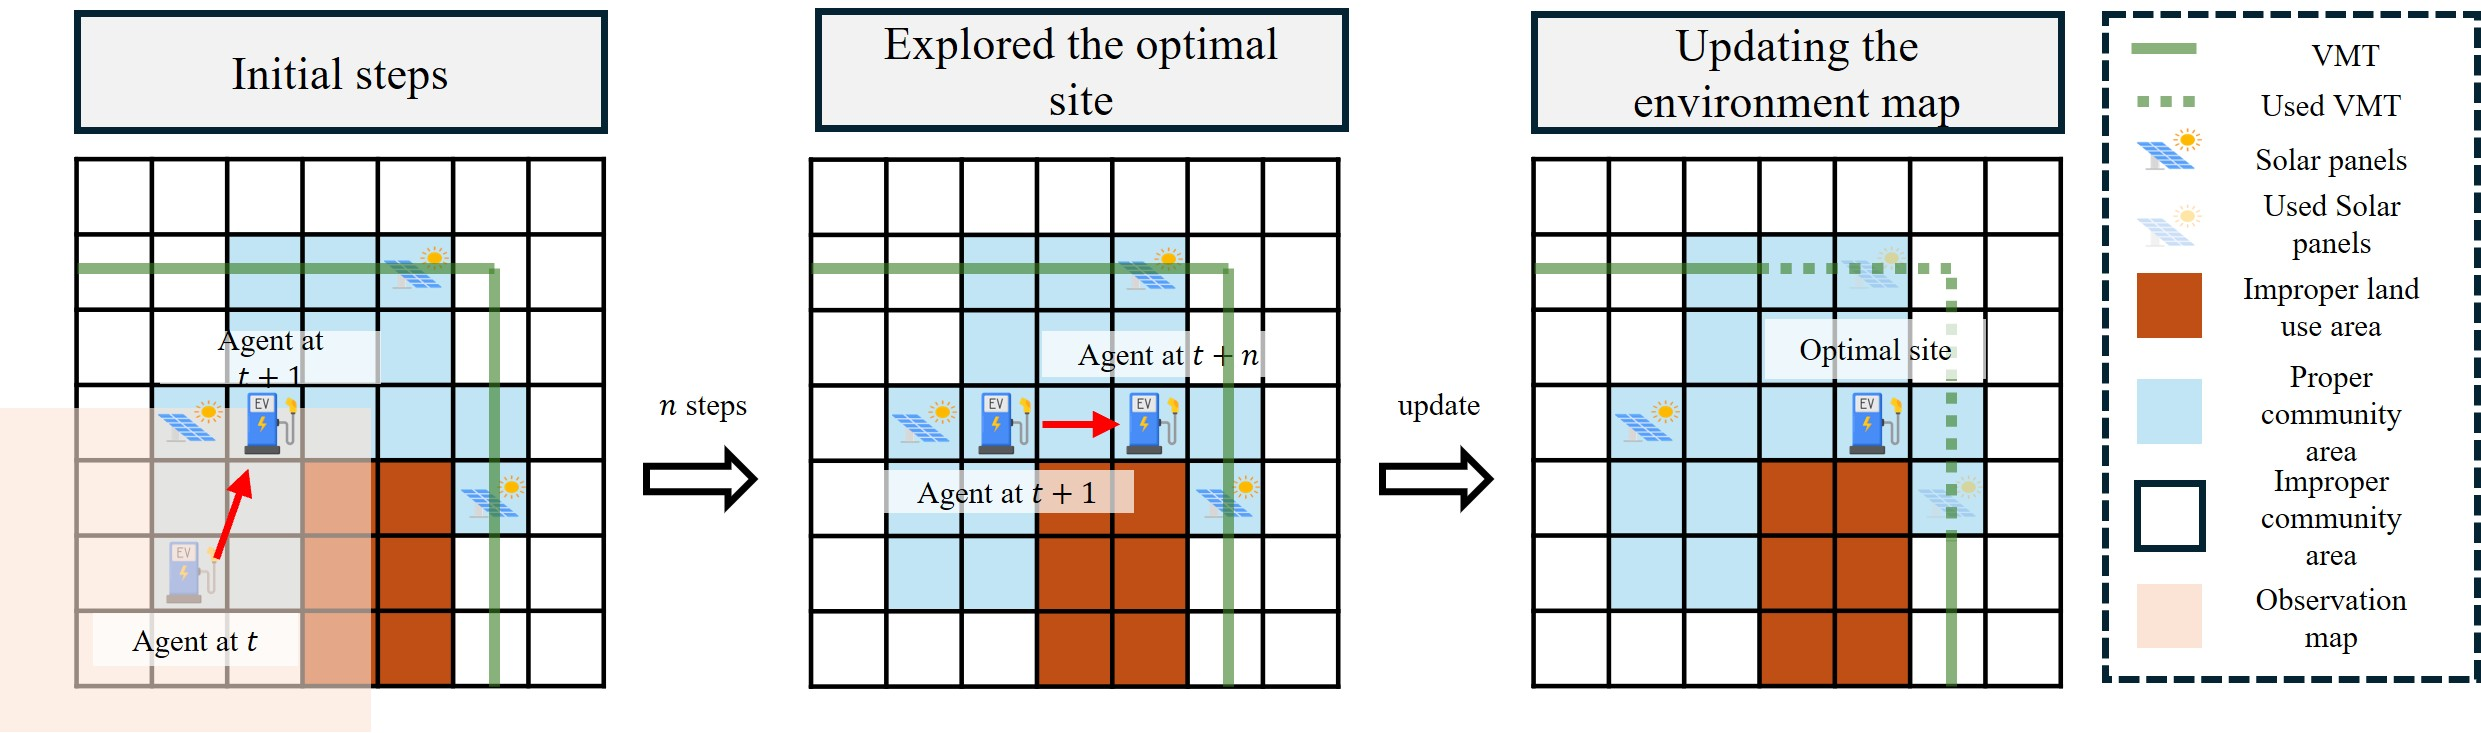
\includegraphics[width=0.85\linewidth]{paper/doc/result_figure/system_model_v3.jpg}
    \caption{Simulated example of overall decision-making strategy in the MODRL}
    \label{fig:seofsm}
\end{figure}
It is an overview of decision-making strategy in a single episode. At the beginning of the time step, the agent observes its limited environment, partially observable map, and selects an action based on its policy. The environment responds by returning a reward and the next state. The agent then iteratively searches for optimal locations that maximize rewards across three objectives while avoiding constraint violations, such as improper land use or high vegetation density. If an optimal site is identified before reaching the maximum time step (i.e., 200), the episode terminates early; otherwise, it continues until the time limit is reached. Upon successfully deploying an EVFCS, the environment map is updated to reflect changes in the spatial distribution of supply and demand, as well as any environmental impact (e.g., vegetation deterioration) resulting from the new charging station. 

\section{Results}
Hyperparameter settings play a critical role in shaping the agent's learning process and determining the overall success of the algorithm. In our study, agents were required to explore the optimal locations 
from varying starting points in each episode without being provided with explicit goals. This setup induces variability and inconsistent learning performance (i.e., instability) in the value function. Moreover, due to the stochastic environment, rewards were often sparsely distributed, further complicating the agent's ability to learn an effective policy. To handle these challenges and enhance the adaptability of RL in a dynamic environment consisting of 77 distinct tasks (i.e., 77 communities), we identified the best hyperparameters through trial and error. These included the learning rates of the actor and critic networks, batch size, clipping coefficient ($\epsilon$), L2 regularization coefficient for the critic ($c_v^{(i)}$), and the entropy regularization coefficient ($c_e$). The final set of optimized hyperparameters is presented in \textcolor{red}{Table} \ref{table:hps}

\begin{table}[h]
    \centering
    \caption{Best hyperparameter settings for actor and critic learning}
    \label{table:hps}
    {\small  % You can use \small, \footnotesize, or \scriptsize
    \resizebox{0.4\textwidth}{!}{  % Shrink the table to 70% of the text width
    \begin{tabular}{ll}
        \toprule
        \textbf{Hyperparameter} & \textbf{Value} \\
        \midrule
        Actor learning rate            & $2 \times 10^{-4}$ \\
        Critic learning rate           & $5 \times 10^{-5}$ \\
        Batch size                     & 50 \\
        L2 regularization (critic)     & $1 \times 10^{-3}$ \\
        Clipping epsilon ($\epsilon$)  & 0.2 \\
        Entropy coefficient ($c_e$)    & 0.05 \\
        Entropy decay rate             & 0.99 \\
        \bottomrule
    \end{tabular}
    }}
\end{table}

Notably, we used a relatively low learning rate for the critic network ($5\times10^{-5}$) to ensure stable estimation of the state-value function. To further prevent overfitting, we incorporated L2 regularization in the critic's optimization process, updating the parameters as $\theta_{i} \gets \theta_{i} - \eta\cdot \frac{\partial L}{\partial \theta_{i}} - \eta\cdot\lambda\cdot\theta_{i}$. The regularization term $\eta\cdot\lambda\cdot\theta_{i}$ penalizes large weights, promoting smoother value function estimates, preventing to gradient exploding and improving generalization performance across tasks. 

\vspace{0.5pt}

To evaluate the effectiveness of the MORL approach, we monitored the reward trajectories and loss graphs. The performance was assessed based on learning stability, convergence behavior, and reward curve. Overall, single policy-based MORL demonstrated enhanced performance through the increasing of average reward values over episodes, as shown in \textcolor{red}{Figure} \ref{fig:trlgsmorl}-(a). 

\begin{figure}[htb]
    \centering
    \subfloat[\centering]{{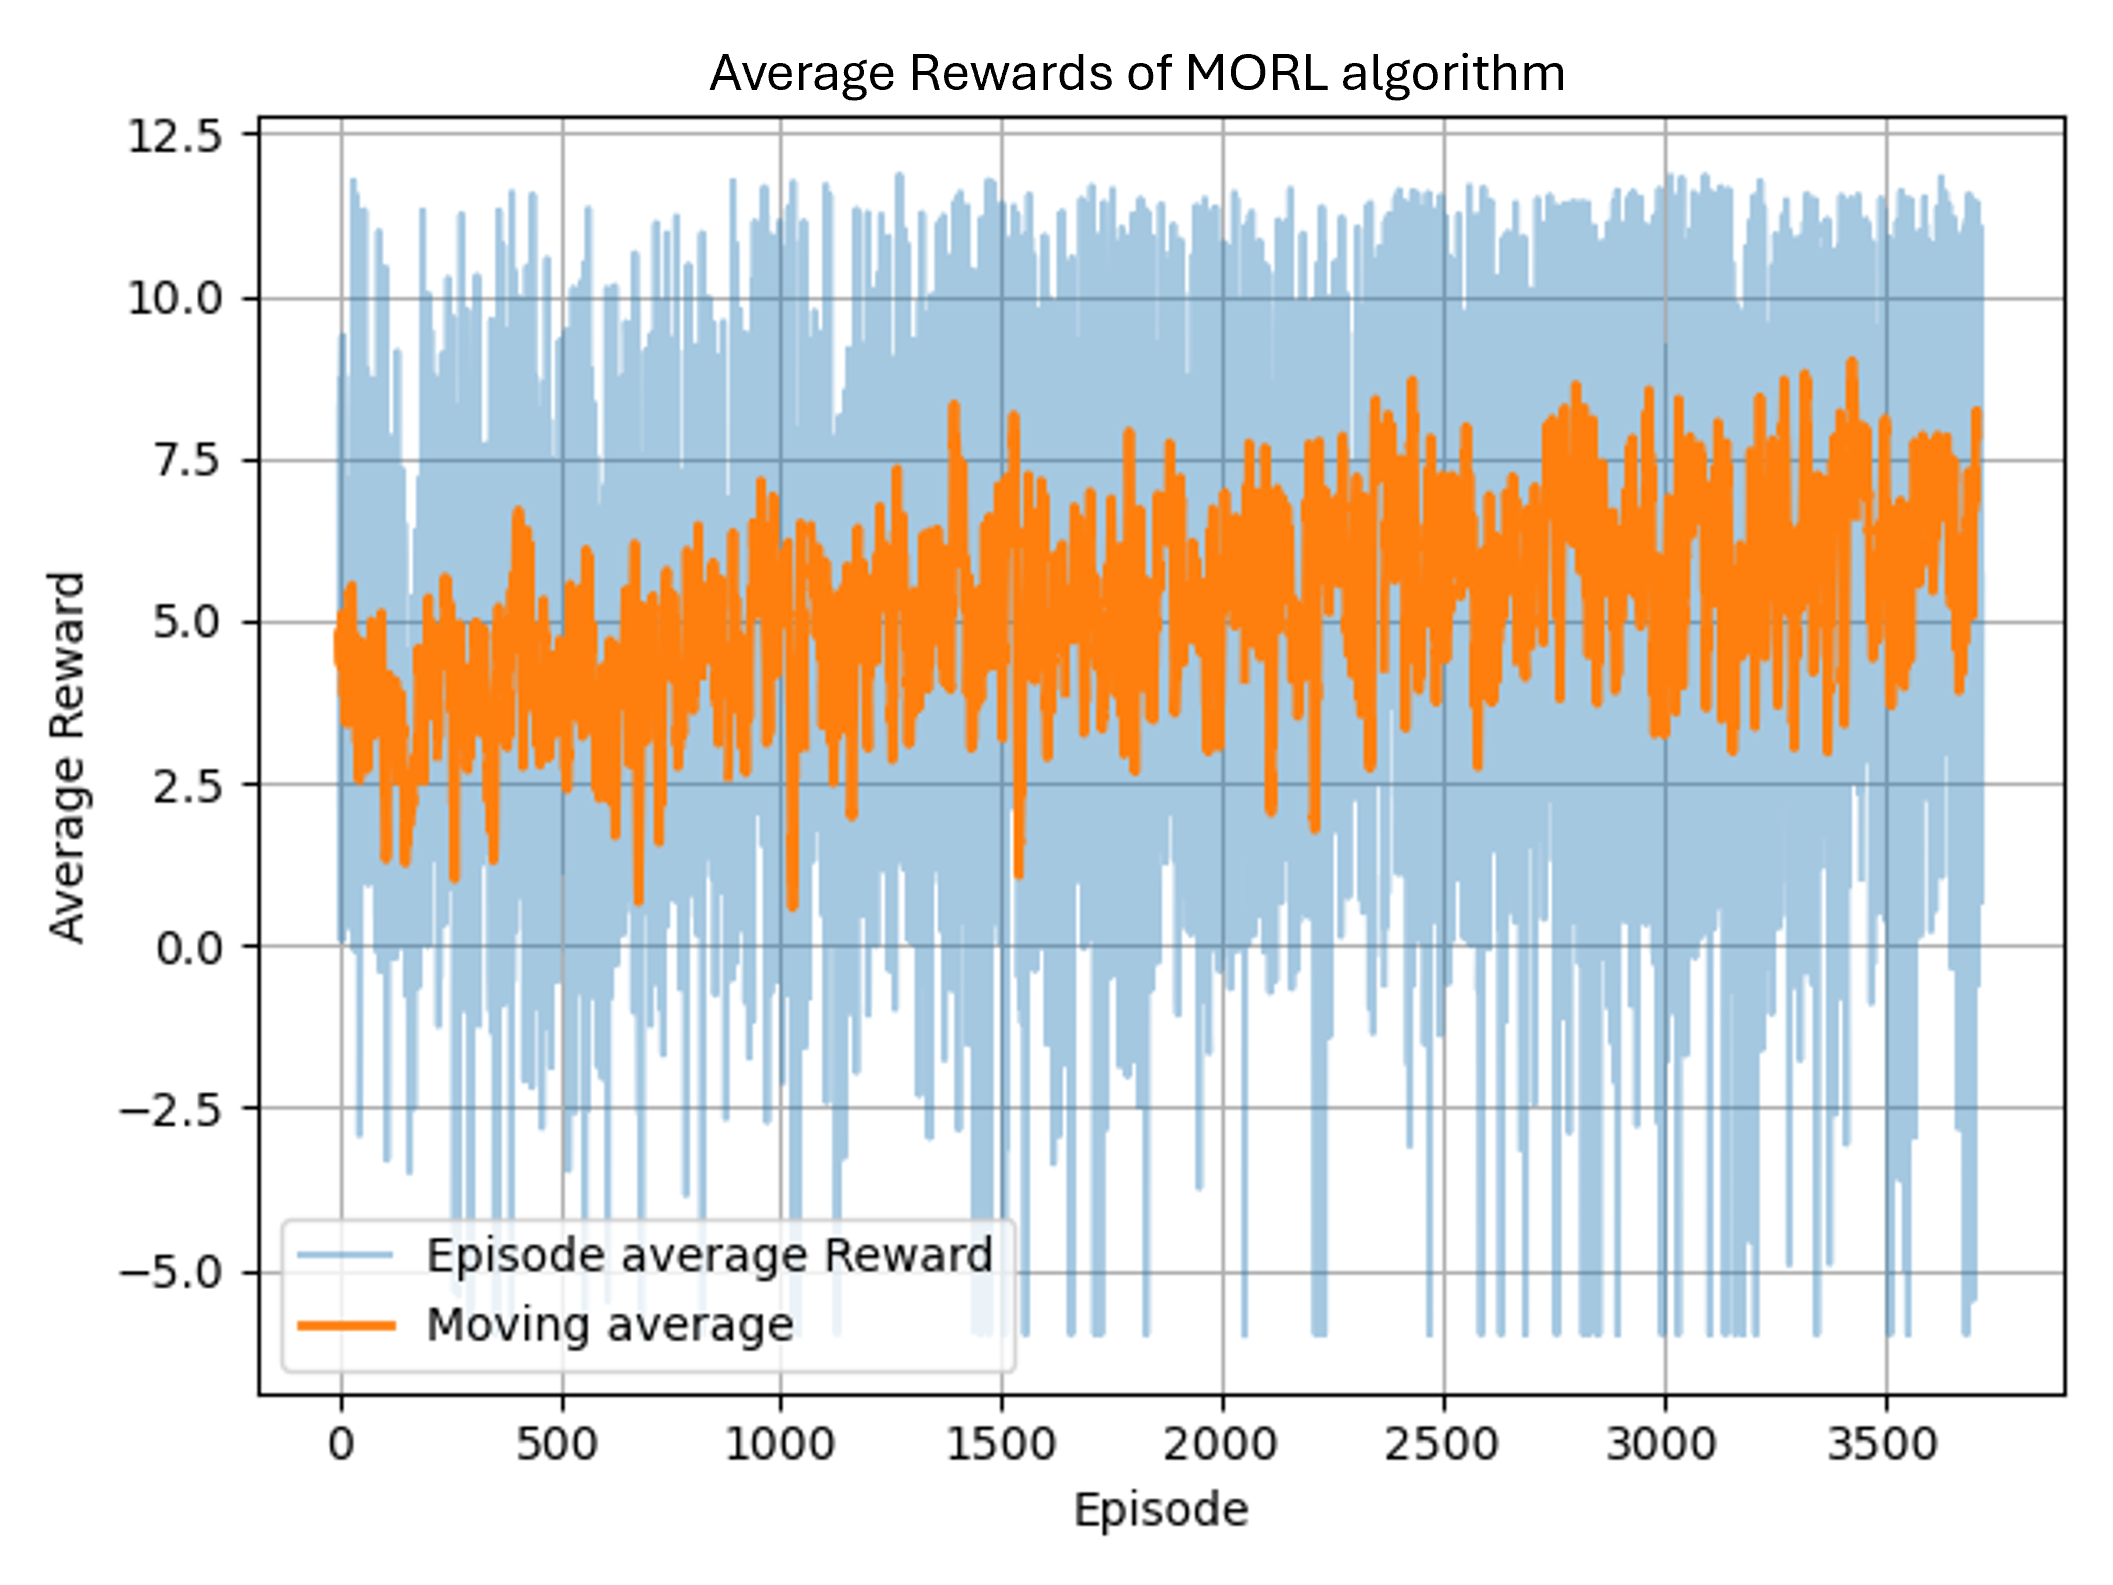
\includegraphics[width=0.25\linewidth]{paper/doc/result_figure/MORL_avg_reward_result_v1.png}}}%
    \qquad
    \hskip -5ex
    \subfloat[\centering]{{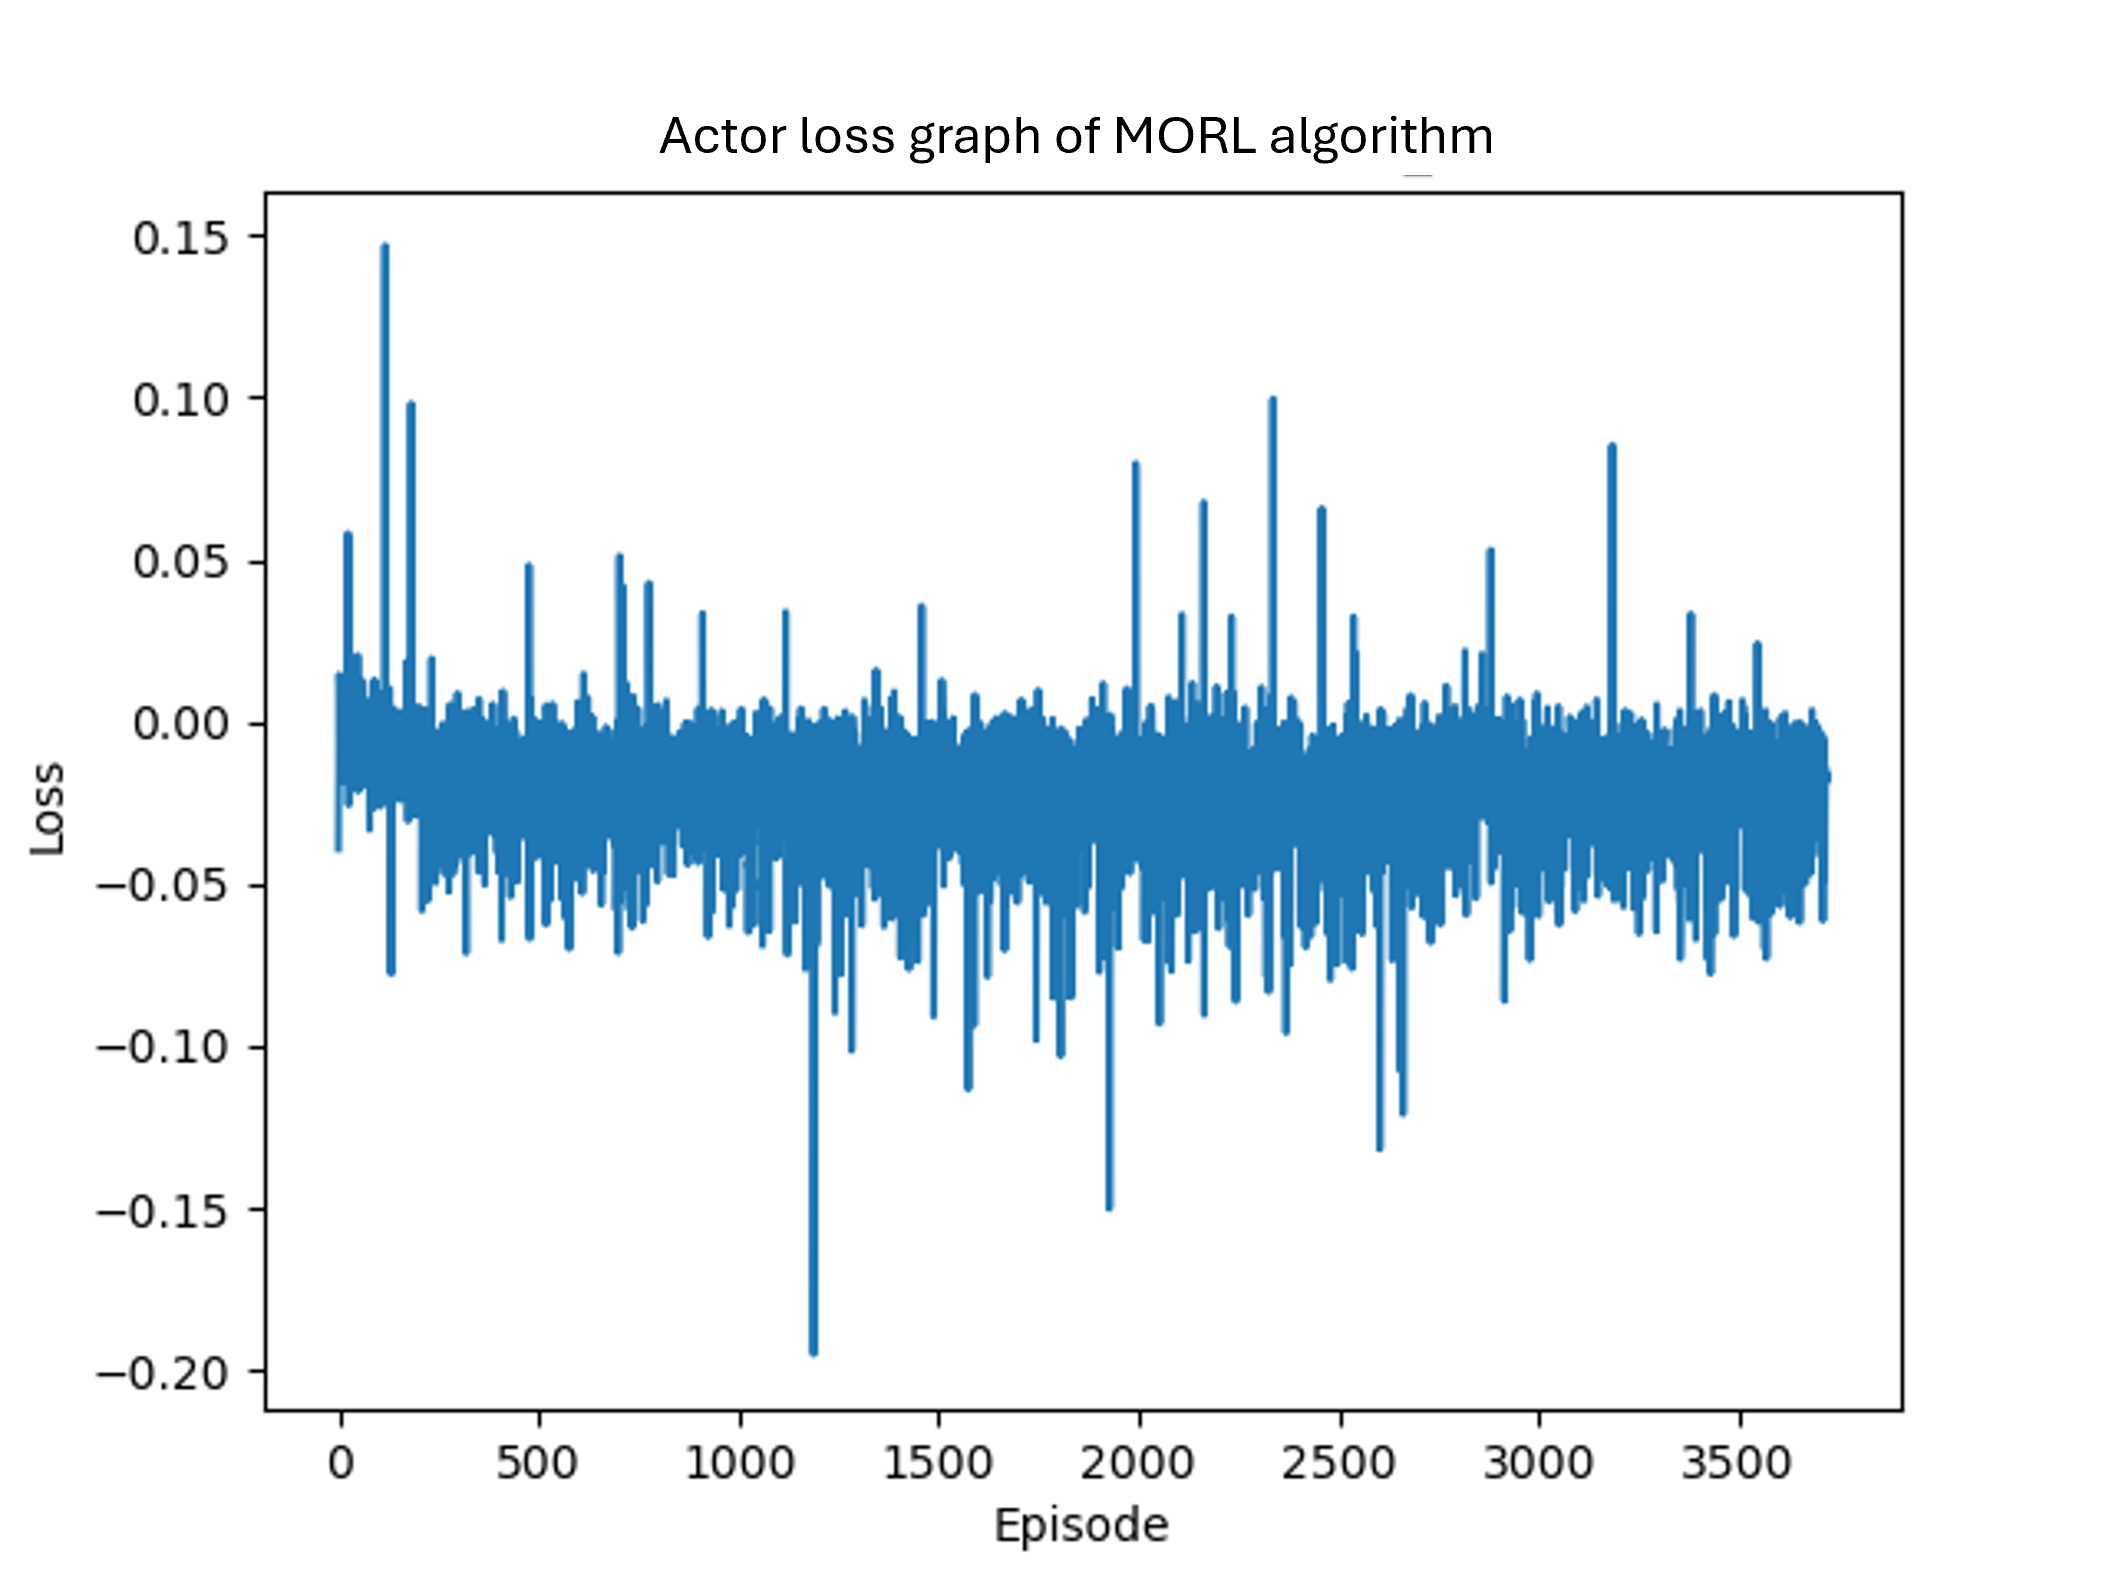
\includegraphics[width=0.25\linewidth]{paper/doc/result_figure/MORL_actor loss_result_v1.png}}}%
    \qquad
    \hskip -5ex
    \subfloat[\centering]{{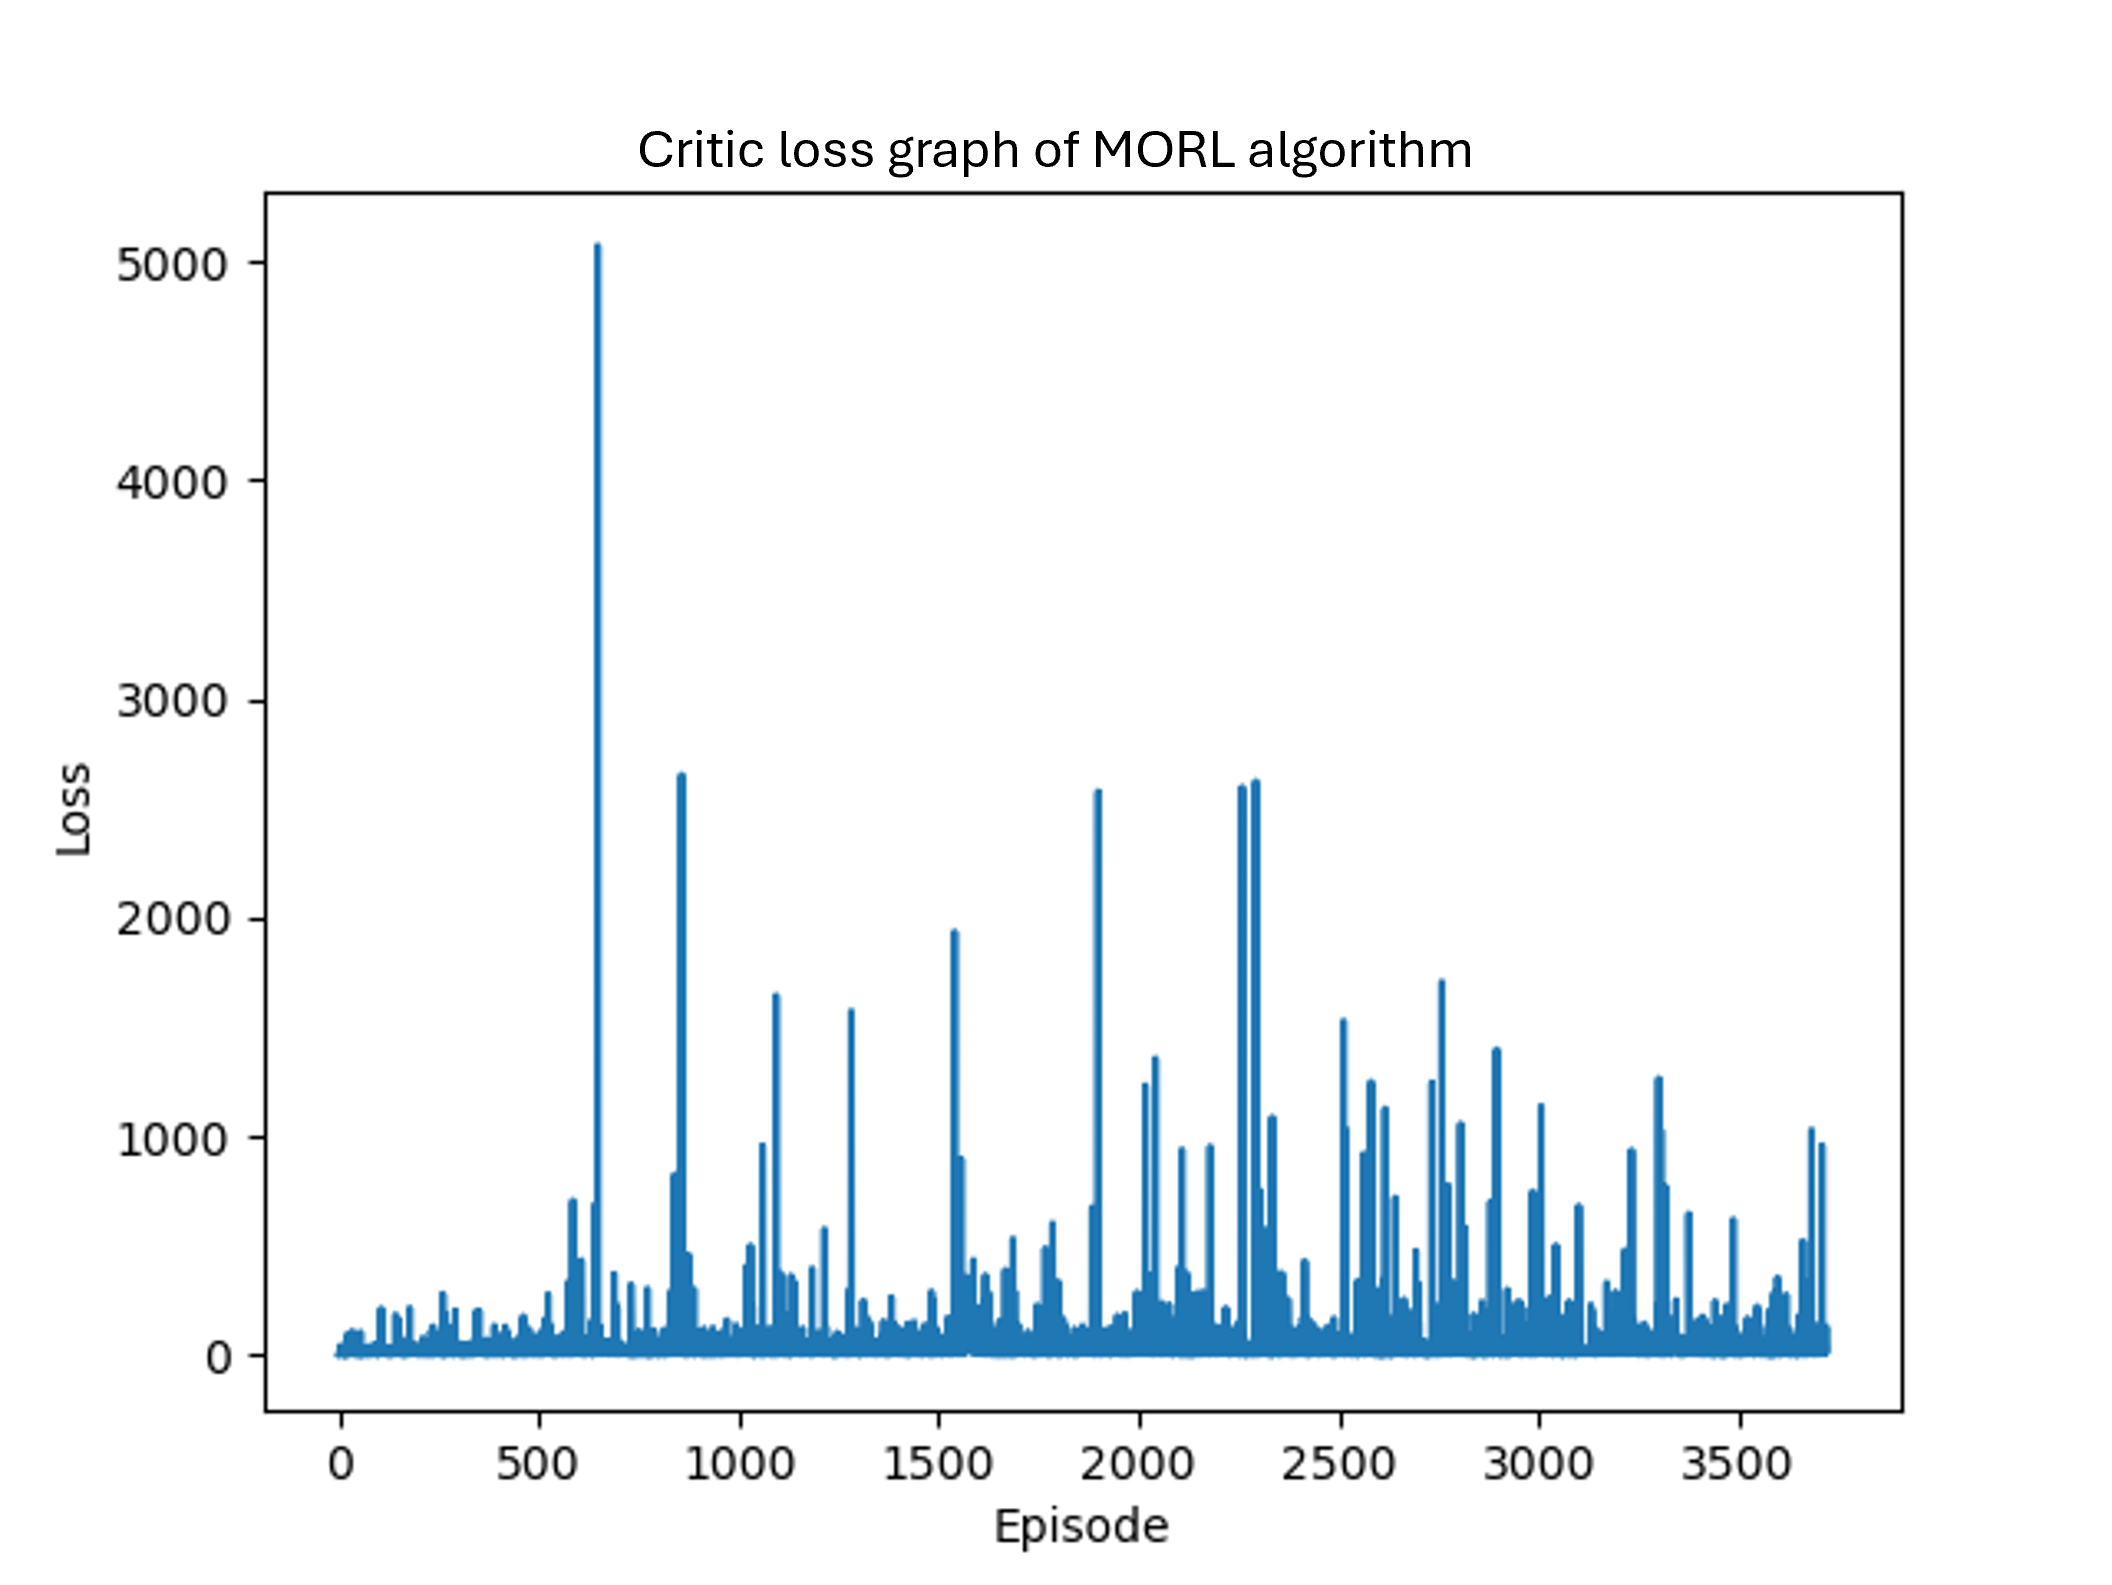
\includegraphics[width=0.25\linewidth]{paper/doc/result_figure/MORL_critic loss_result_v1.png}}}%
    \qquad
    \hskip -5ex
    \subfloat[\centering]{{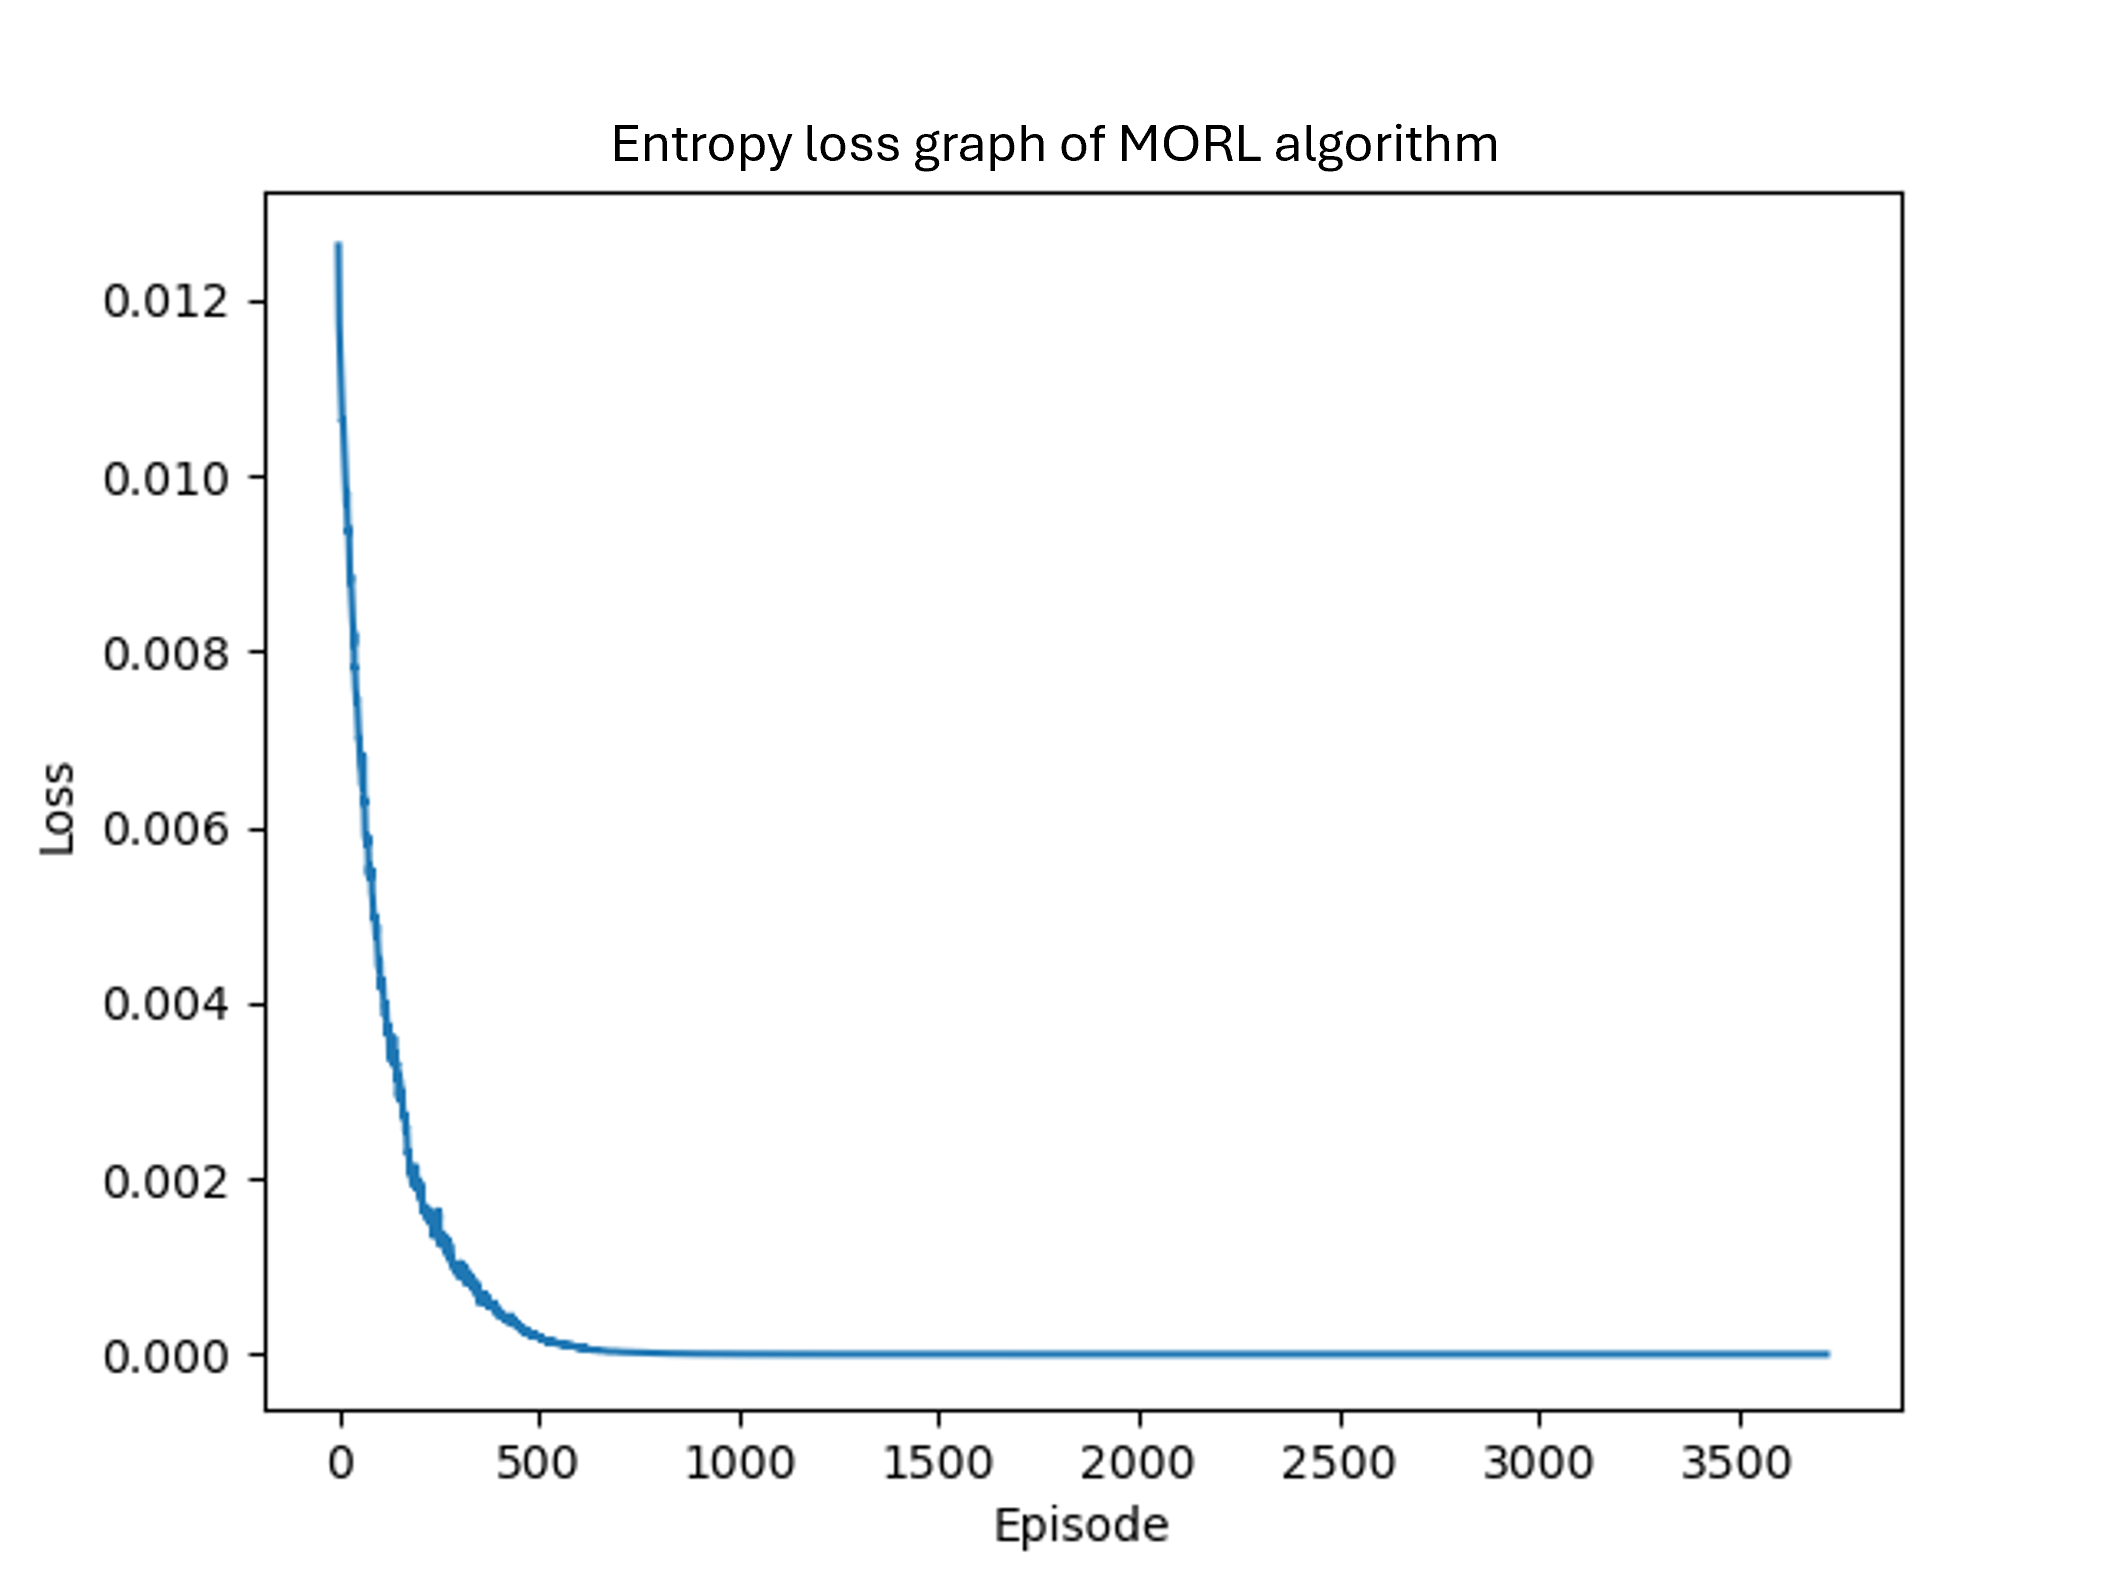
\includegraphics[width=0.25\linewidth]{paper/doc/result_figure/MORL_entropy loss_result_v1.png}}}%
    
    \captionsetup{format=plain, font=small, labelfont=bf}
    \caption{Training reward and loss graphs using MORL algorithm: (a) average reward graph, (b) actor loss graph, (c) critic loss graph, and (d) entropy loss graph}
    \label{fig:trlgsmorl}
\end{figure}

For example, the moving average reward initially ranged from 2.5 to 5.0 during early training and later improved to a range of 5.0 to 7.5, approximately two times higher than the initial performance. This improvement indicates that the agent, operating in a complex and inconsistent environment, successfully learned the strategy for optimal placement of EVFCS in efficient sequential decisions. As learning progresses, the model enables the agent to explore optimal sites, where all objectives (i.e., Q-values) are satisfied. Our MORL PPO algorithm showed three primary loss graphs to verify whether the model has converged to a reseanable solution: (b) actor loss, (c) critic loss, and (d) entropy loss, showed that the agent has learned an effective policy, as shown in \textcolor{red}{Figure} \ref{fig:trlgsmorl}-(b-d). The actor (policy), \textcolor{red}{Figure} \ref{fig:trlgsmorl}-(b) loss quantifies how much the current policy improves sample efficiency compared to the old policy. During the initial training phase (episodes 1-100), the actor loss increased as the agent explored extensively and made substantial updates based on the advantage signals. After approximately 100 episodes, the actor loss began to decrease and eventually stabilized near zero. It implies that the policy has converged to the optimal policy and does not need to be further adjusted. In other words, the model may find the optimal decision-making strategy. The critic loss \textcolor{red}{Figure} \ref{fig:trlgsmorl}-(c), which measures the mean squared error (MSE) between predicted and actual returns, remained mostly low and stable. However, occasional spikes (e.g., around episodes 630 and 870) were observed due to the sparse rewards-based environment, which occasionally limited effective value estimation, and might not have a goal in a task. Lastly, the entropy loss reflects the balance between exploration (high entropy) and exploitation (low entropy) in the agent's action distribution. Early in training, the agent exhibited high entropy, reflecting random exploratory actions. After around episode 600, the entropy loss approached zero, indicating that the agent had shifted to a deterministic strategy. It implies that the model has converged toward an optimal policy.  

\vspace{0.5cm}

As one of the MORL frameworks, the multiple-policy-based asynchronous federated reinforcement learning model was built and evaluated using four average reward graphs: the global model (a) and three local models corresponding to the (b) environmental, (c) economic, and (d) urbanity policies, as shown in \textcolor{red}{Figure}\ref{fig:trgafrlm}-(a-d). 

\begin{figure}[htb]
    \centering
    \subfloat[\centering]{{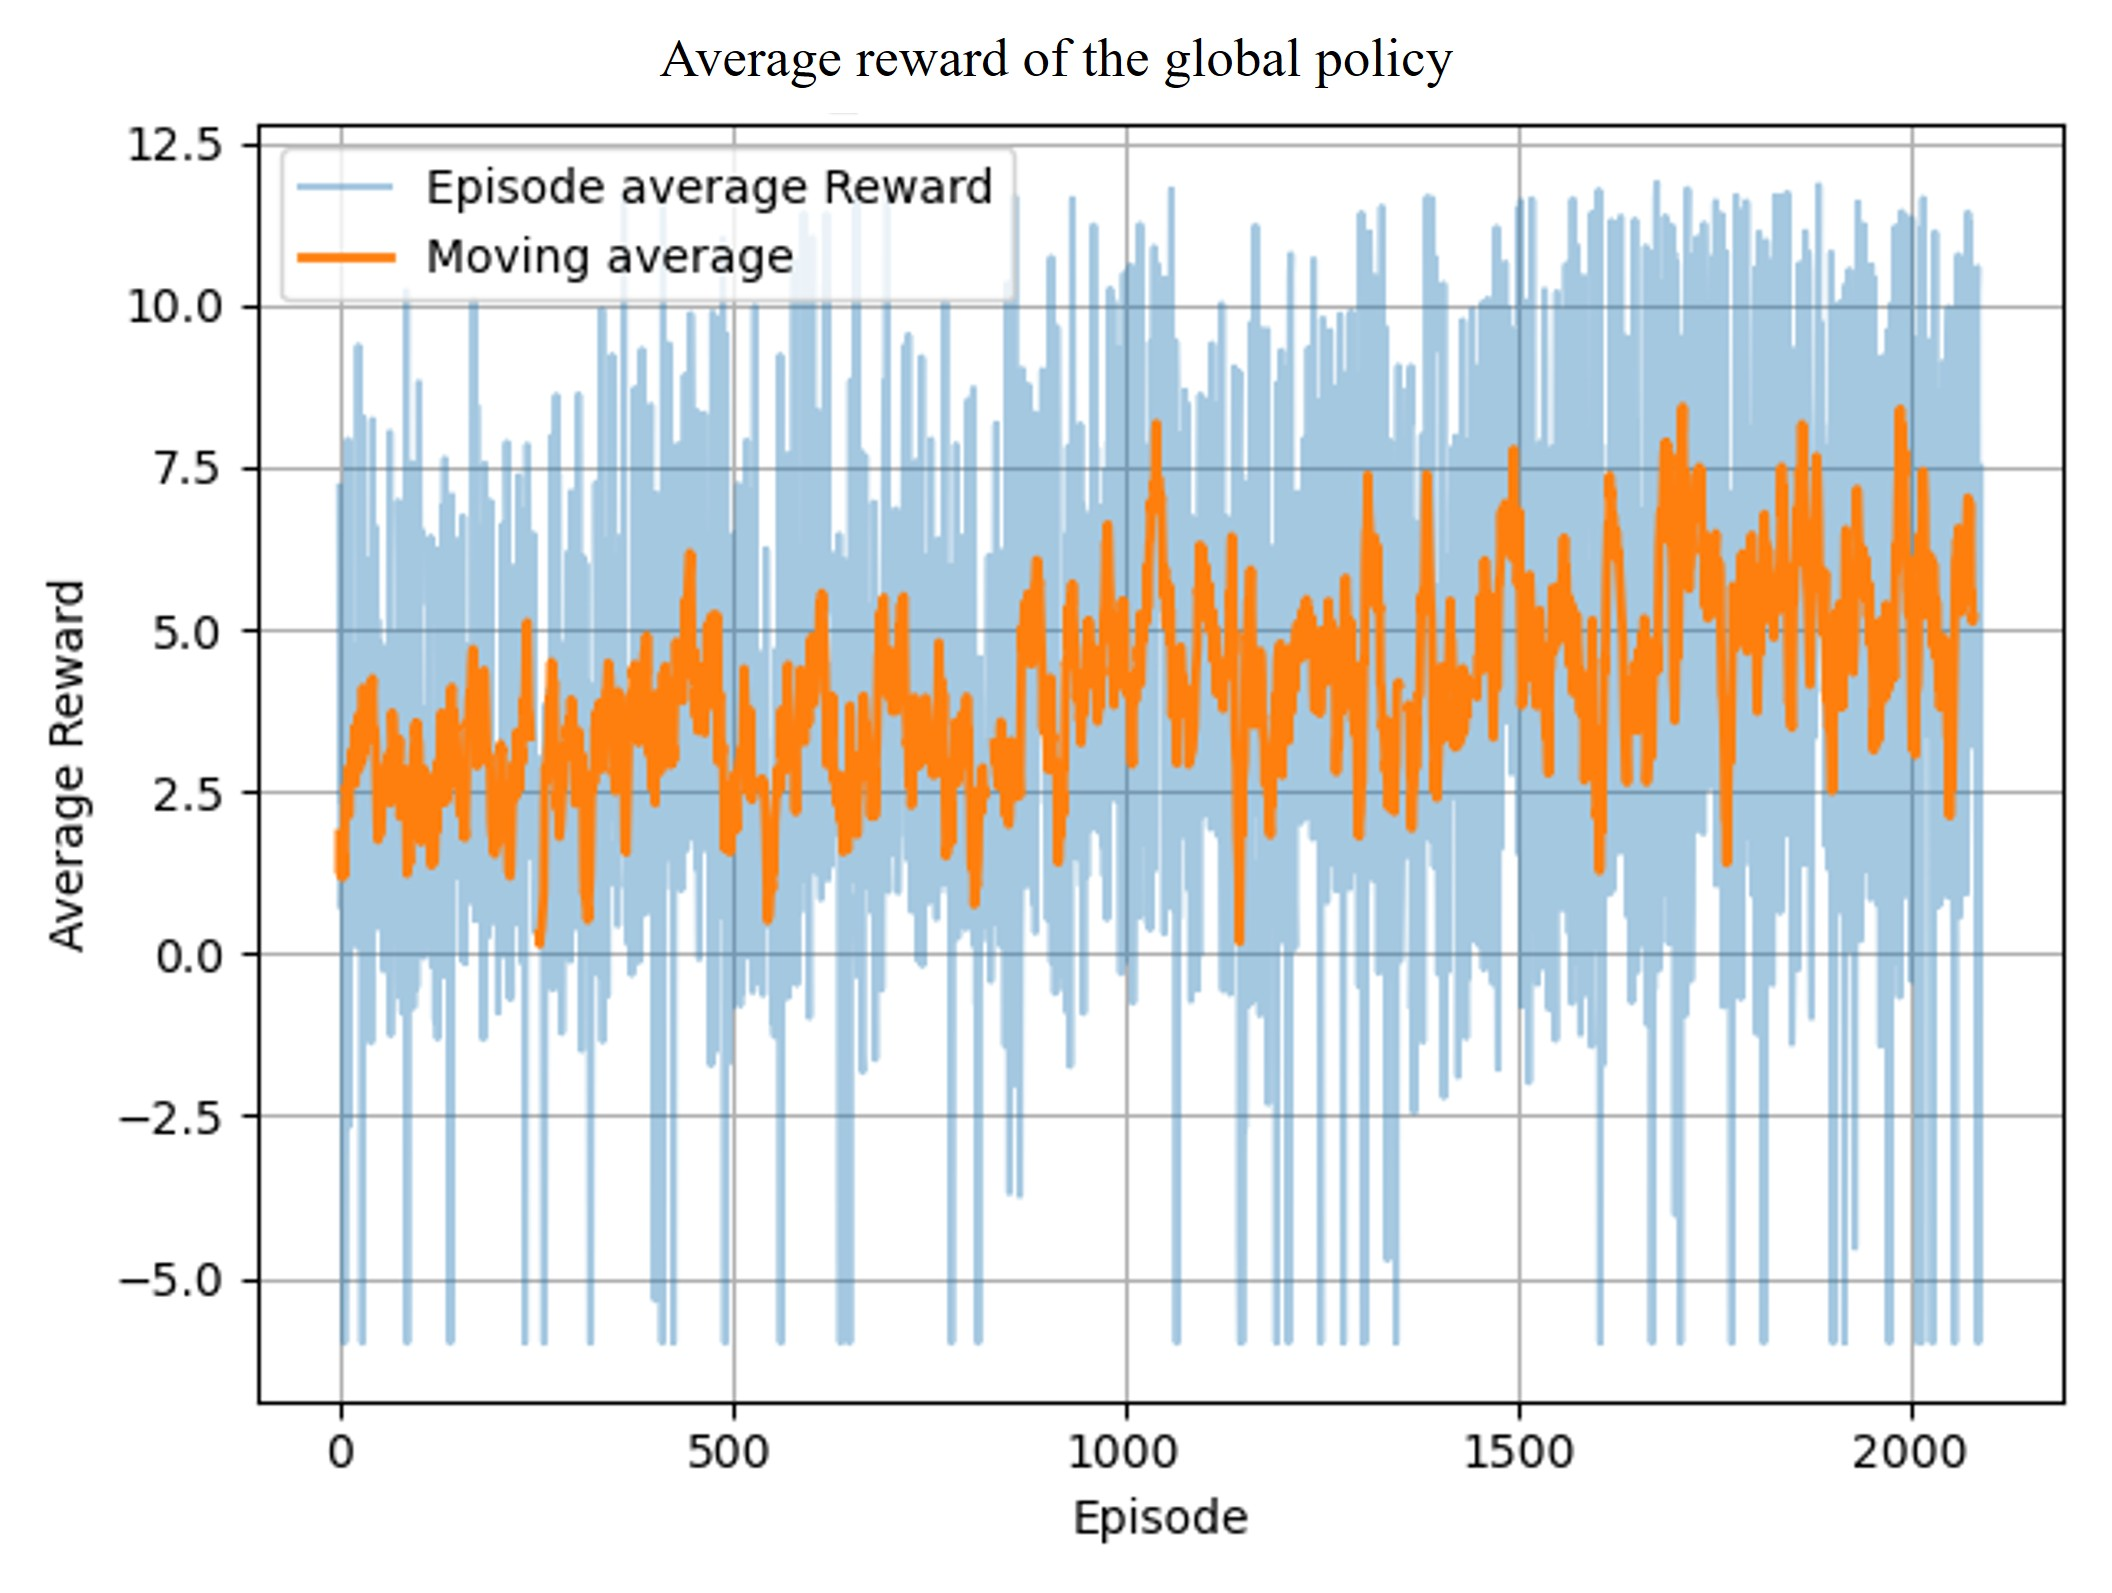
\includegraphics[width=0.25\linewidth]{paper/doc/result_figure/AFMORL_global_avg_re_v2.jpg}}}%
    \qquad
    \hskip -7ex
    \subfloat[\centering]{{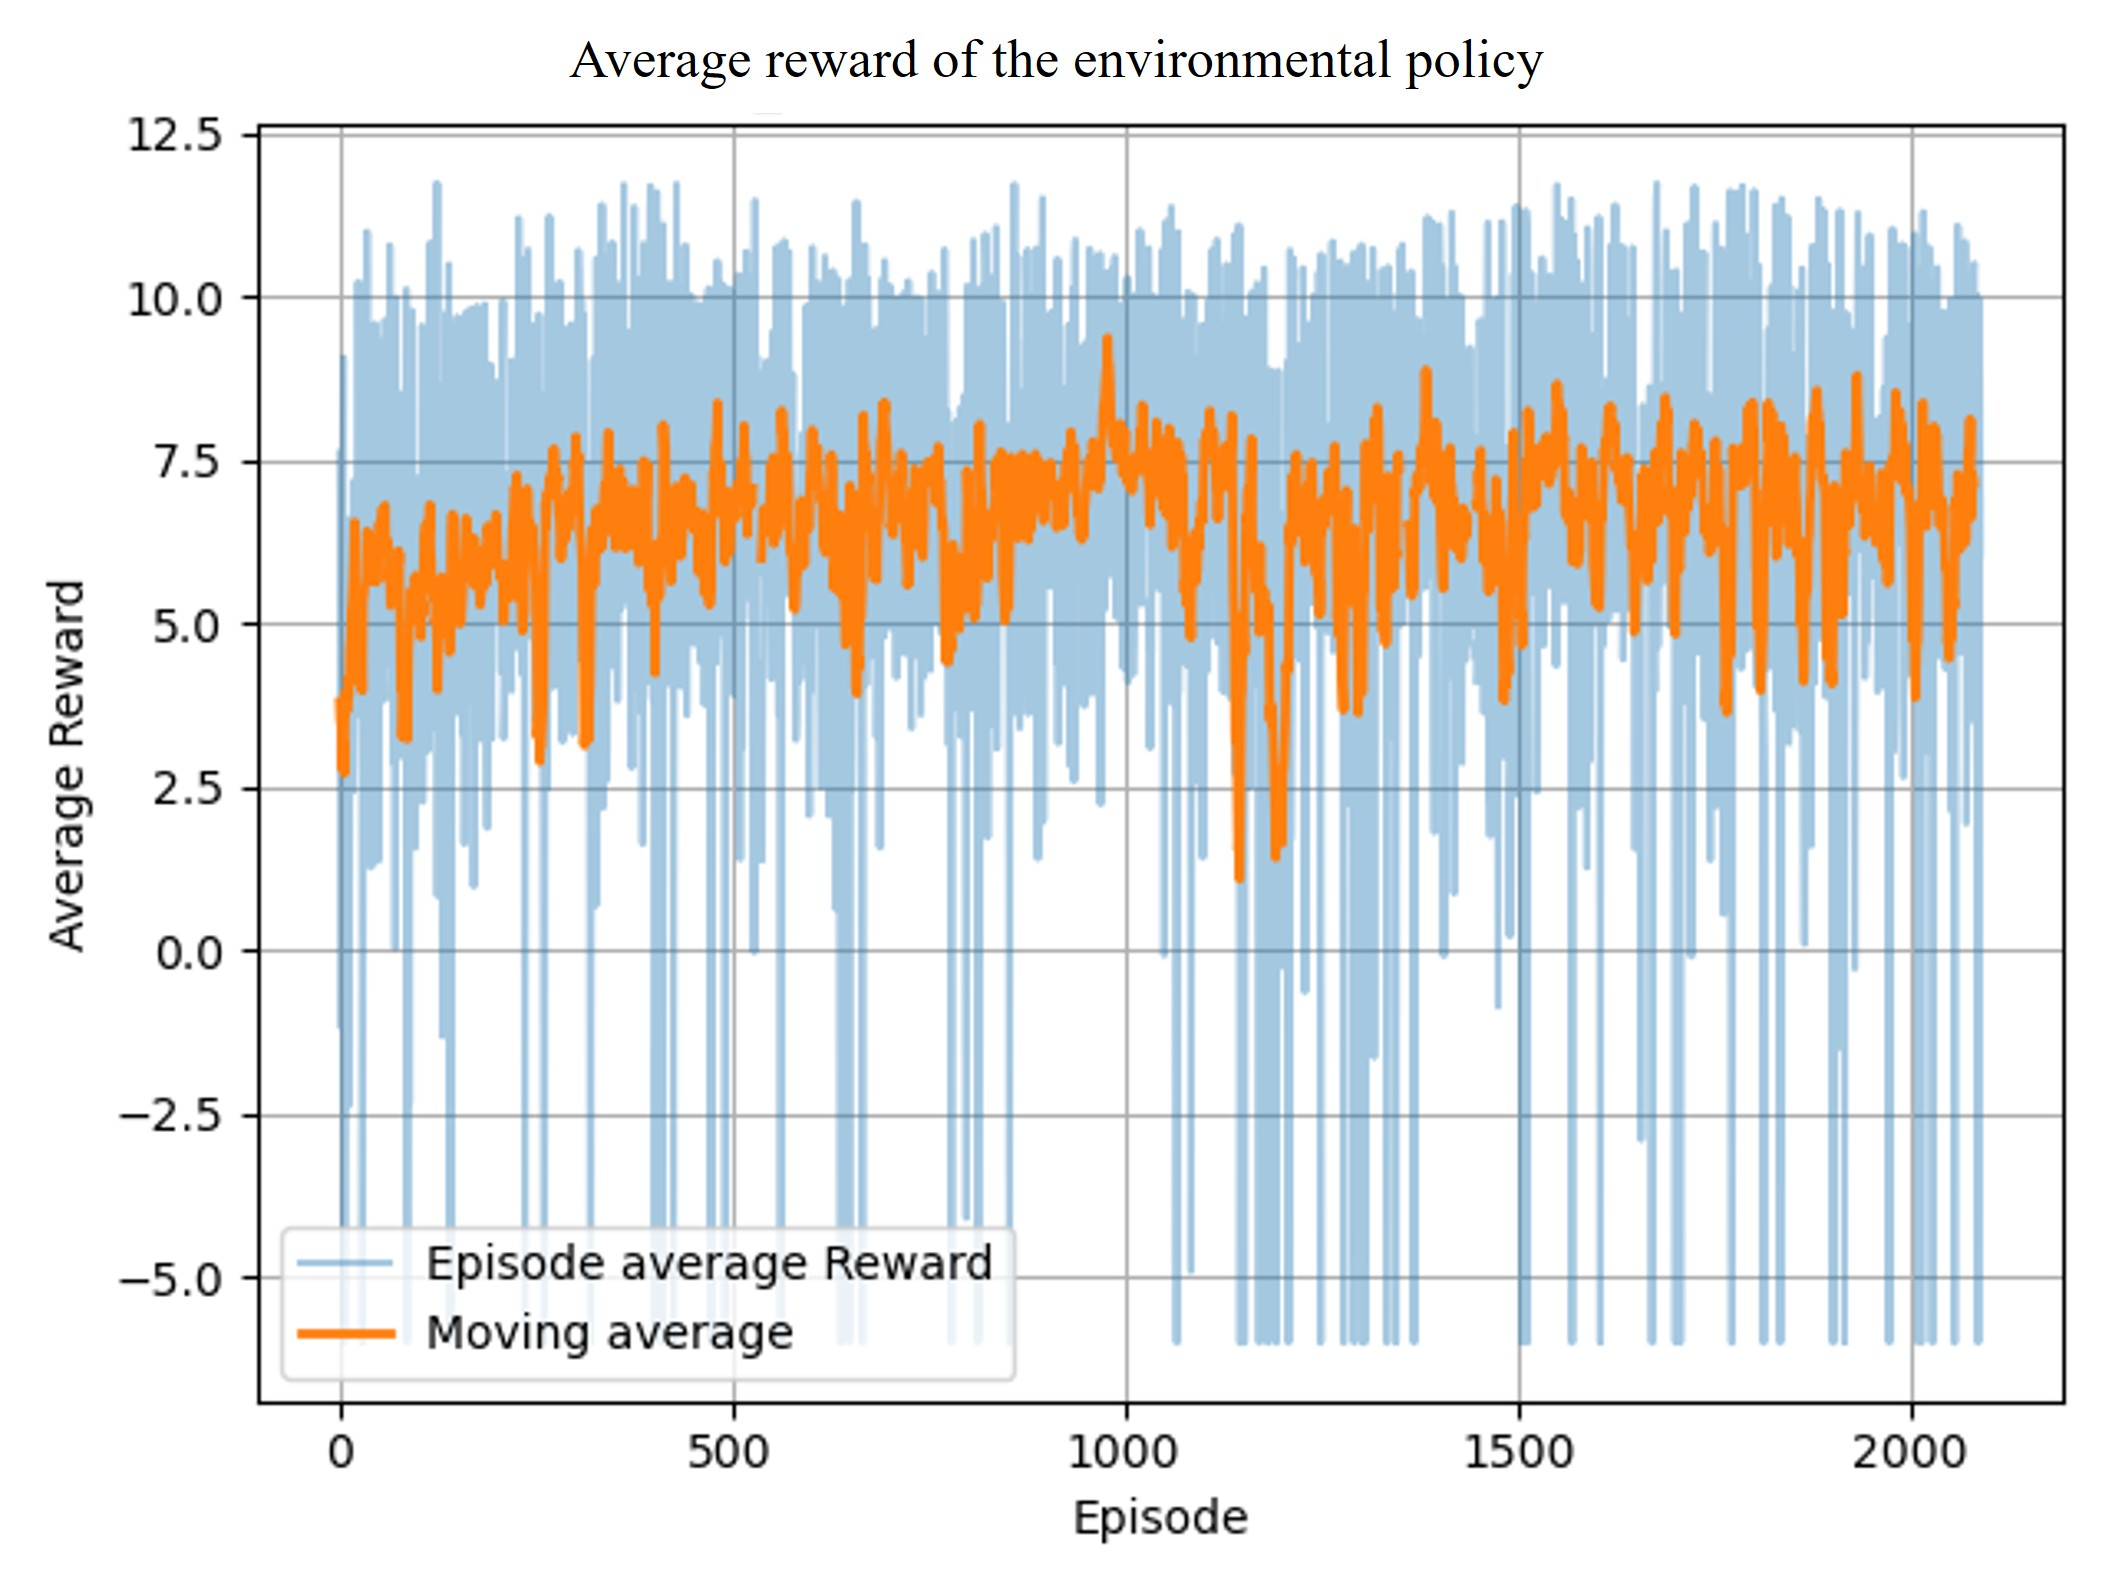
\includegraphics[width=0.25\linewidth]{paper/doc/result_figure/AFMORL_env_avg_re_v2.jpg}}}%
    \qquad
    \hskip -7ex
    \subfloat[\centering]{{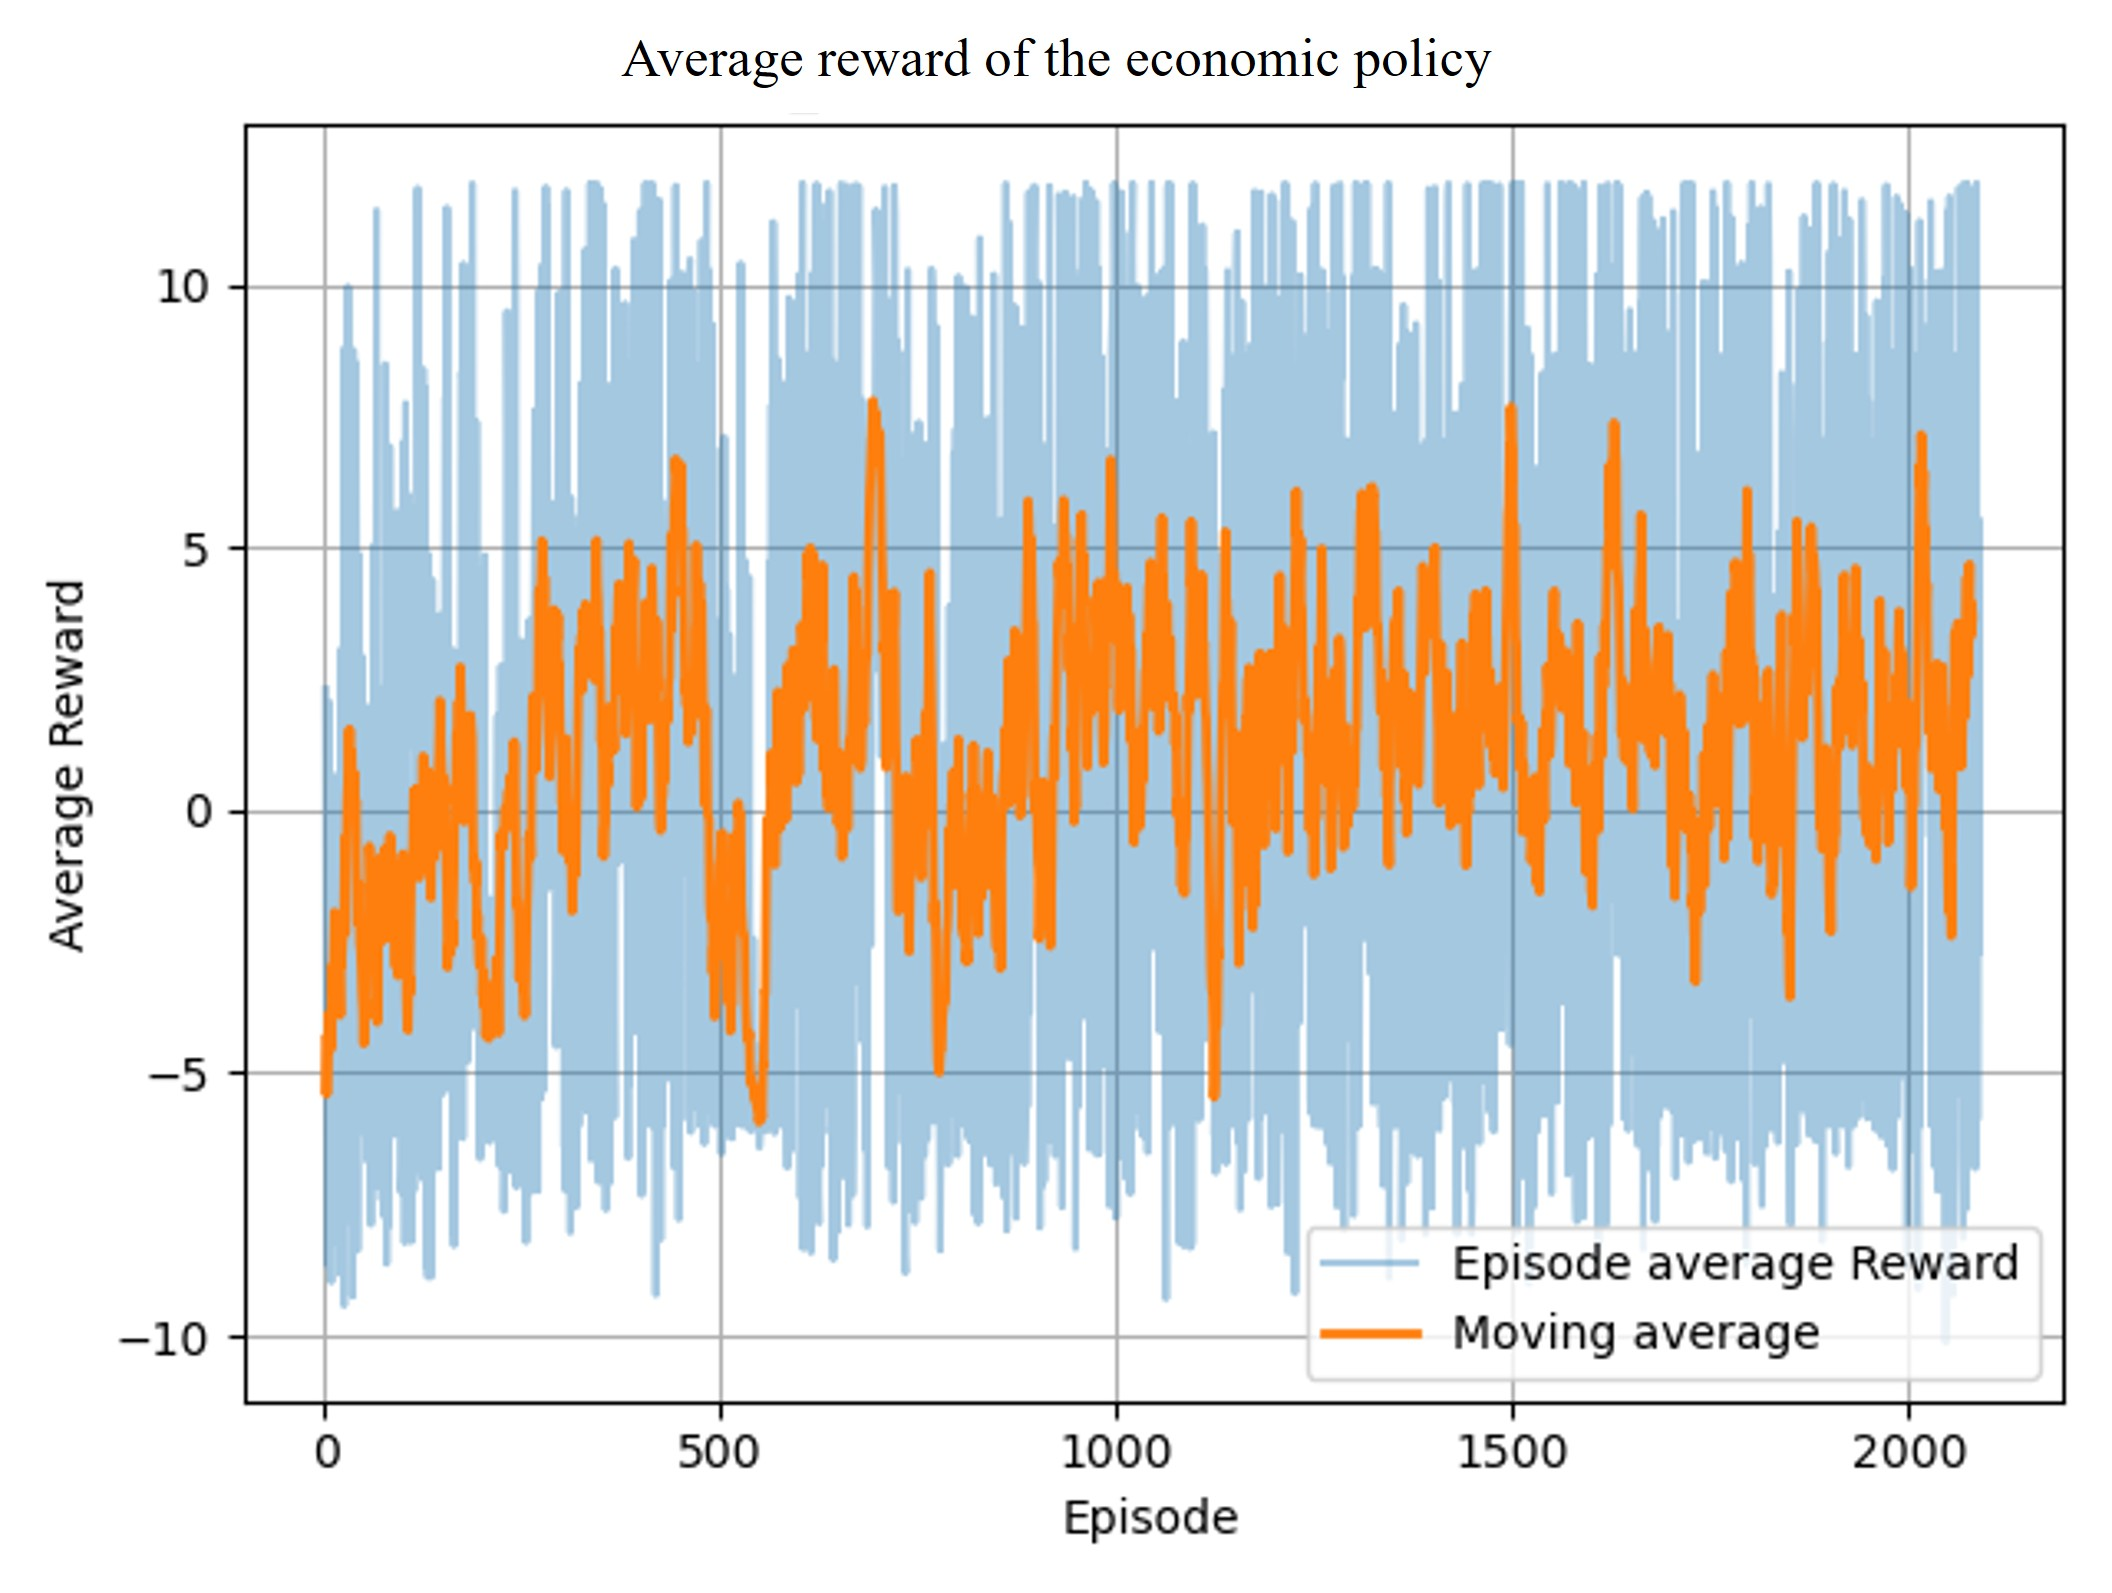
\includegraphics[width=0.25\linewidth]{paper/doc/result_figure/AFMORL_eco_avg_re_v2.jpg}}}%
    \qquad
    \hskip -7ex
    \subfloat[\centering]{{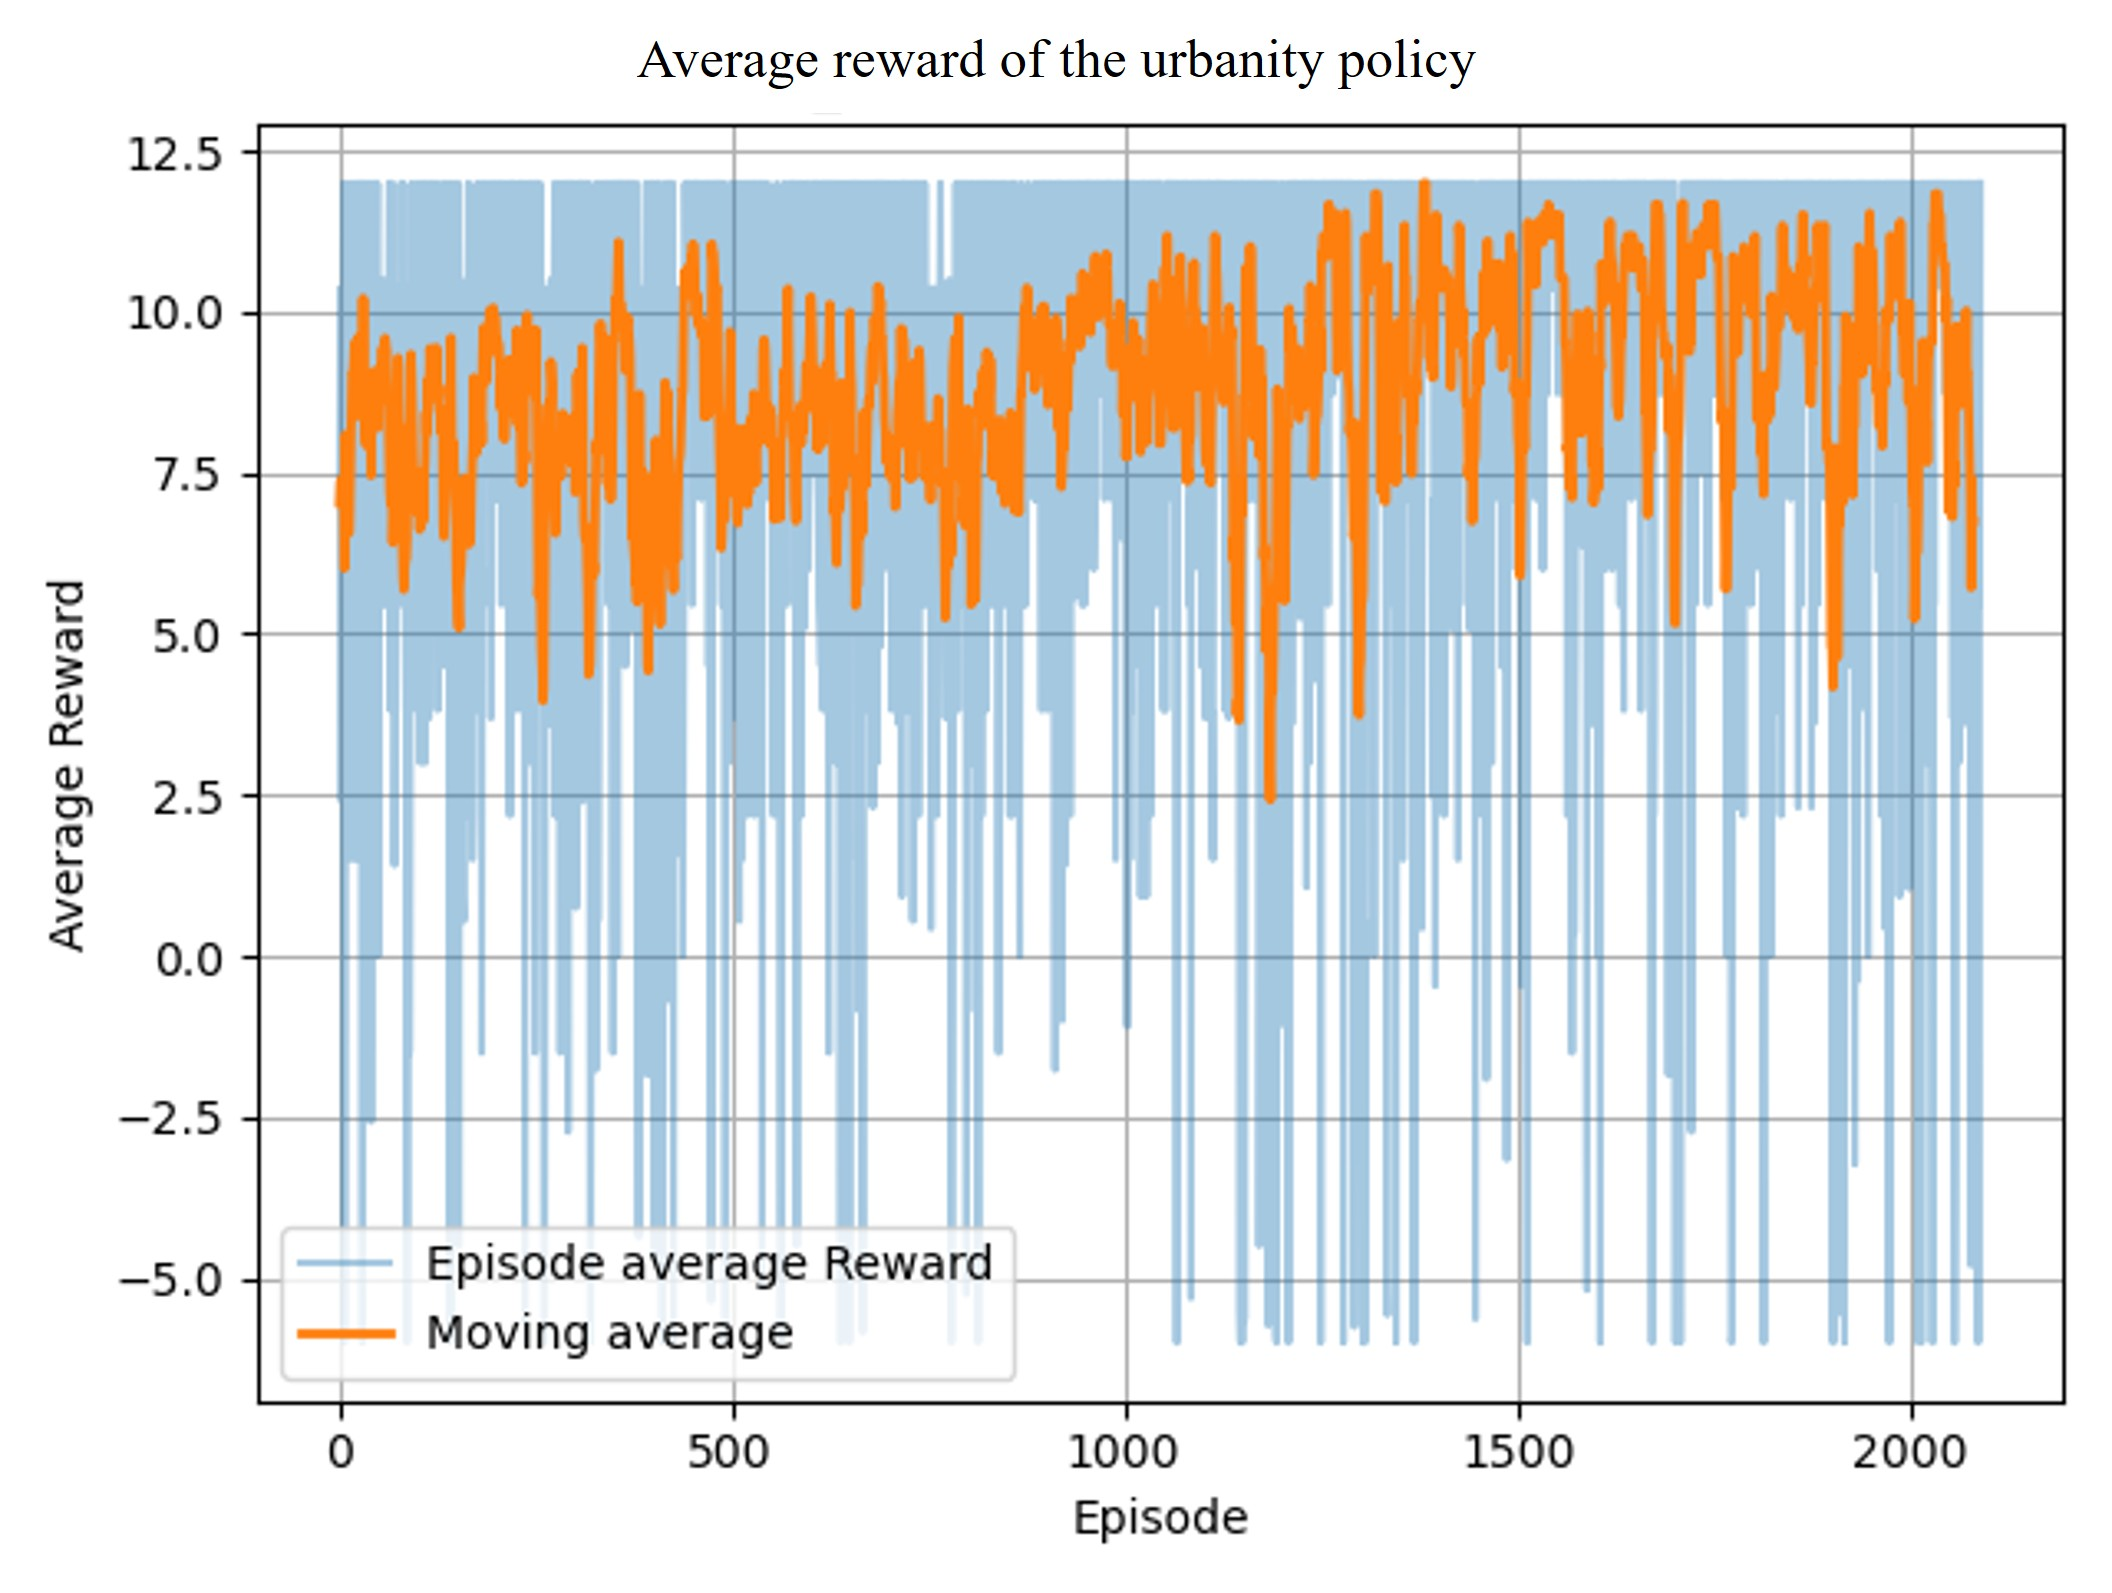
\includegraphics[width=0.25\linewidth]{paper/doc/result_figure/AFMORL_urbanity_avg_re_v2.jpg}}}%
    
    \captionsetup{format=plain, font=small, labelfont=bf}
    \caption{Training reward graphs of (a) global model and three local models; (b) environmental, (c) economic, and (d) urbanity: Average reward (blue line), and moving average reward (red line)}
    \label{fig:trgafrlm}
\end{figure}

In the local models, three models have different learning performance. Overall, all rewards and learning performance (reward and actor loss graph) are consistently increased in all objectives. For instance, the environmental model shows that the agent steadily improves its average reward, as shown in \textcolor{red}{Figure \ref{fig:trgafrlm}}-(b). The moving average of the episode increases gradually and converges to values above 7.5. This indicates successful policy learning under the environmental objective. The corresponding critic loss (\textcolor{red}{Appendix A.2}) initially increases and shows high variance around episode 1,000-1,800 due to increasing reward variance. However, it stabilizes toward the end of training, suggesting that the value function approximator eventually aligns with the expected return. The economic objective model reveals slow learning but consistent learning patterns, with the moving average reward increasing from negative values to 5. The critic loss for the economic objective (\textcolor{red}{Appendix A.5}) shows considerable fluctuation, especially in 1,500-2,000 episodes. It may be difficult to predict sparse economic rewards. The urbanity reward learning curve demonstrates a continuous improvement, stabilizing above 9, and has lower variance compared to other objectives. It implies that the agent quickly learns a near-optimal policy for urbanity-focused decisions. The urbanity critic loss (\textcolor{red}{Appendix A.8}) is relatively stable with minor spikes, and the policy loss (\textcolor{red}{Appendix A.7}) demonstrates stable convergence behavior, compared with other objectives. 

Furthermore, the results of the global model demonstrate that our model effectively addresses the EVFCS placement problems. For example, the learning curve of the moving average reward graph increased by approximately 2.5 times over training. Moreover, the improved rewards show that the algorithm successfully achieves the designed average reward range, spanning from -12 to +12, with a threshold of +6, representing the minimum level required to satisfy all objectives. It indicates that the aggregated global model decodes the placement problem by integrating independent local behavior, ultimately identifying optimal locations where all objectives are met. However, the multiple-policy MORL model exhibited lower learning performance and reduced stability compared to the single-policy MORL model, as shown by the reward and loss graphs. Therefore, we opted to select the single policy MORL model as the preferred model for presenting and interpreting the subsequent result analysis.

To conduct an in-depth analysis of the proposed EVFCS placement strategy, we simulated the sequential decision-making process across time steps within a single episode, comparing the outcomes between an early-stage (under-trained) model in \textcolor{red}{Figure \ref{fig:lpdts}}-(a) and a sufficiently trained (optimized) model in \textcolor{red}{Figure \ref{fig:lpdts}}-(b). 

\begin{figure}[htb]
    \centering
    \subfloat[\centering]{{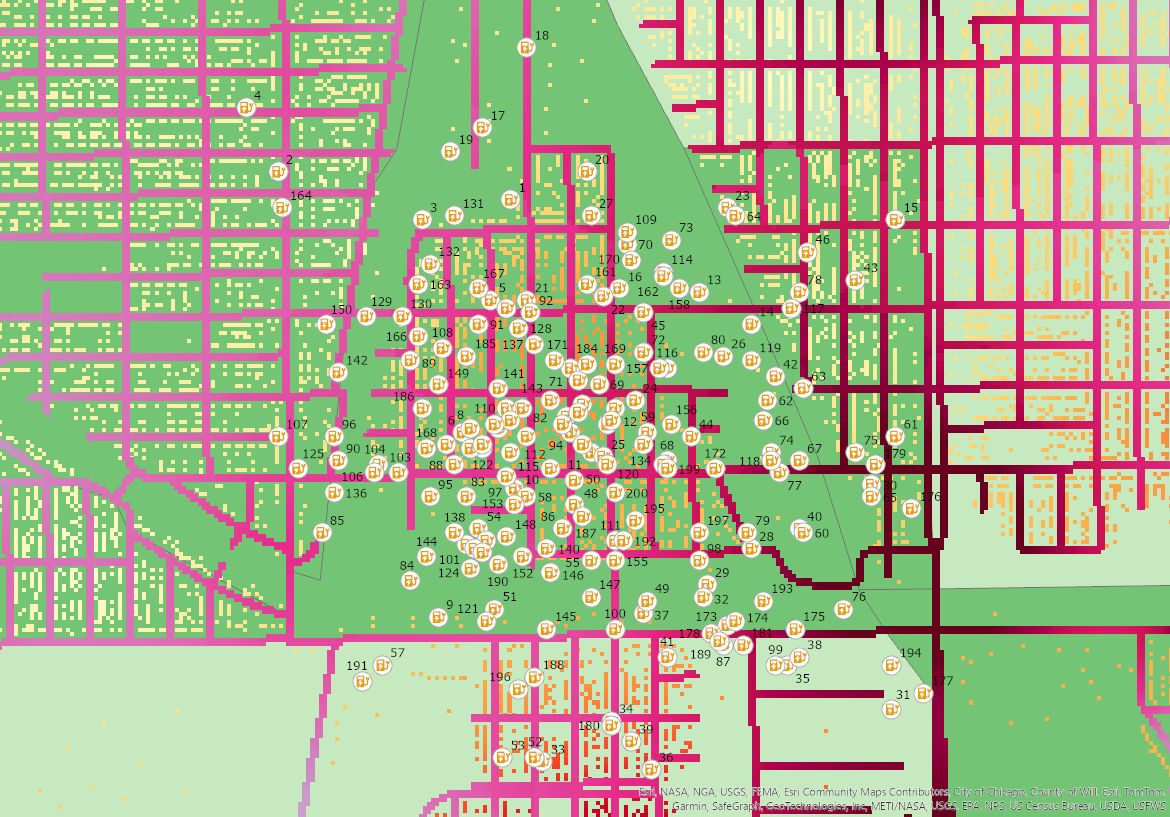
\includegraphics[width=0.33\linewidth]{paper/doc/result_figure/initial_time_step_result_v2.jpg}}}%
    \qquad
    \subfloat[\centering]{{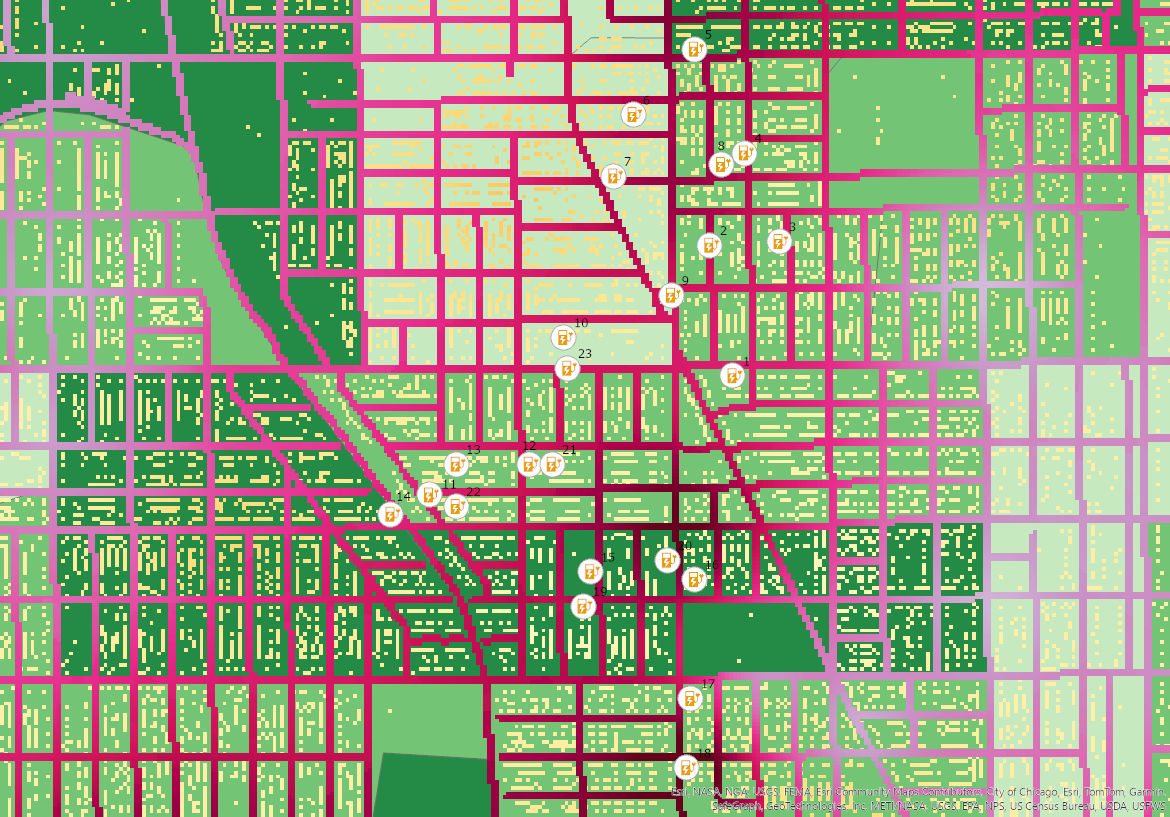
\includegraphics[width=0.33\linewidth]{paper/doc/result_figure/learnt_time_step_results_v2.jpg}}}%

    \captionsetup{format=plain, font=small, labelfont=bf}
    \caption{Learning progress during time steps in (a) under-trained model episode at 10, and (2) optimized model episode at 1,000}
    \label{fig:lpdts}
\end{figure}

The results show that the under-trained model struggled to identify optimal sites and ultimately failed to reach a goal within the maximum number of time steps (i.e., 200). Its learning behavior exhibited aimless exploration around potentially optimal sites. In contrast, the optimized model efficiently identified optimal sites within 23 time steps, demonstrating early stopping behavior. It implies that continued training enables the model to make more accurate decisions and significantly improves the efficiency of the EVFCS site selection process.  

\vspace{0.5cm}

The proposed approach successfully allocates charging stations across urban areas without resulting in an uneven distribution. However, not all episodes can be designated as optimal EVFCS placement sites as some failed to identify suitable locations within maximum number of time steps, particularly when not all objectives were satisfied. To highlight optimal outcomes, we filtered the results using the following thresholds, illustrated in \textcolor{red}{Figure \ref{fig:peloqr}}: (1) episodes with an average reward of all three criteria greater than +6 (blue dots), (2) greater than +8 (bright green dots), and (3) greater than +10 (yellow dots). These thresholds represent scenarios in which all sub-criteria within each main criterion were satisfied. 

\begin{figure}[htb]
    \centering
    \subfloat[\centering]{{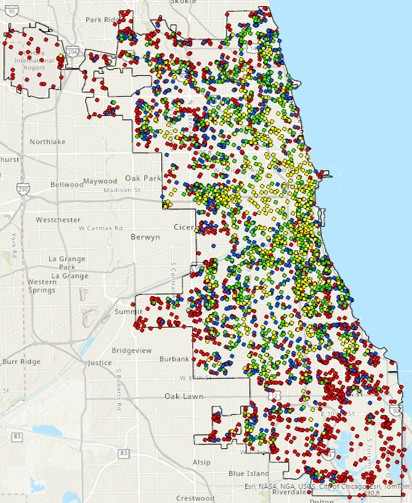
\includegraphics[width=0.25\linewidth]{paper/doc/result_figure/raw_result_map_v4.jpg}}}%
    \qquad
    \hskip -5ex
    \subfloat[\centering]{{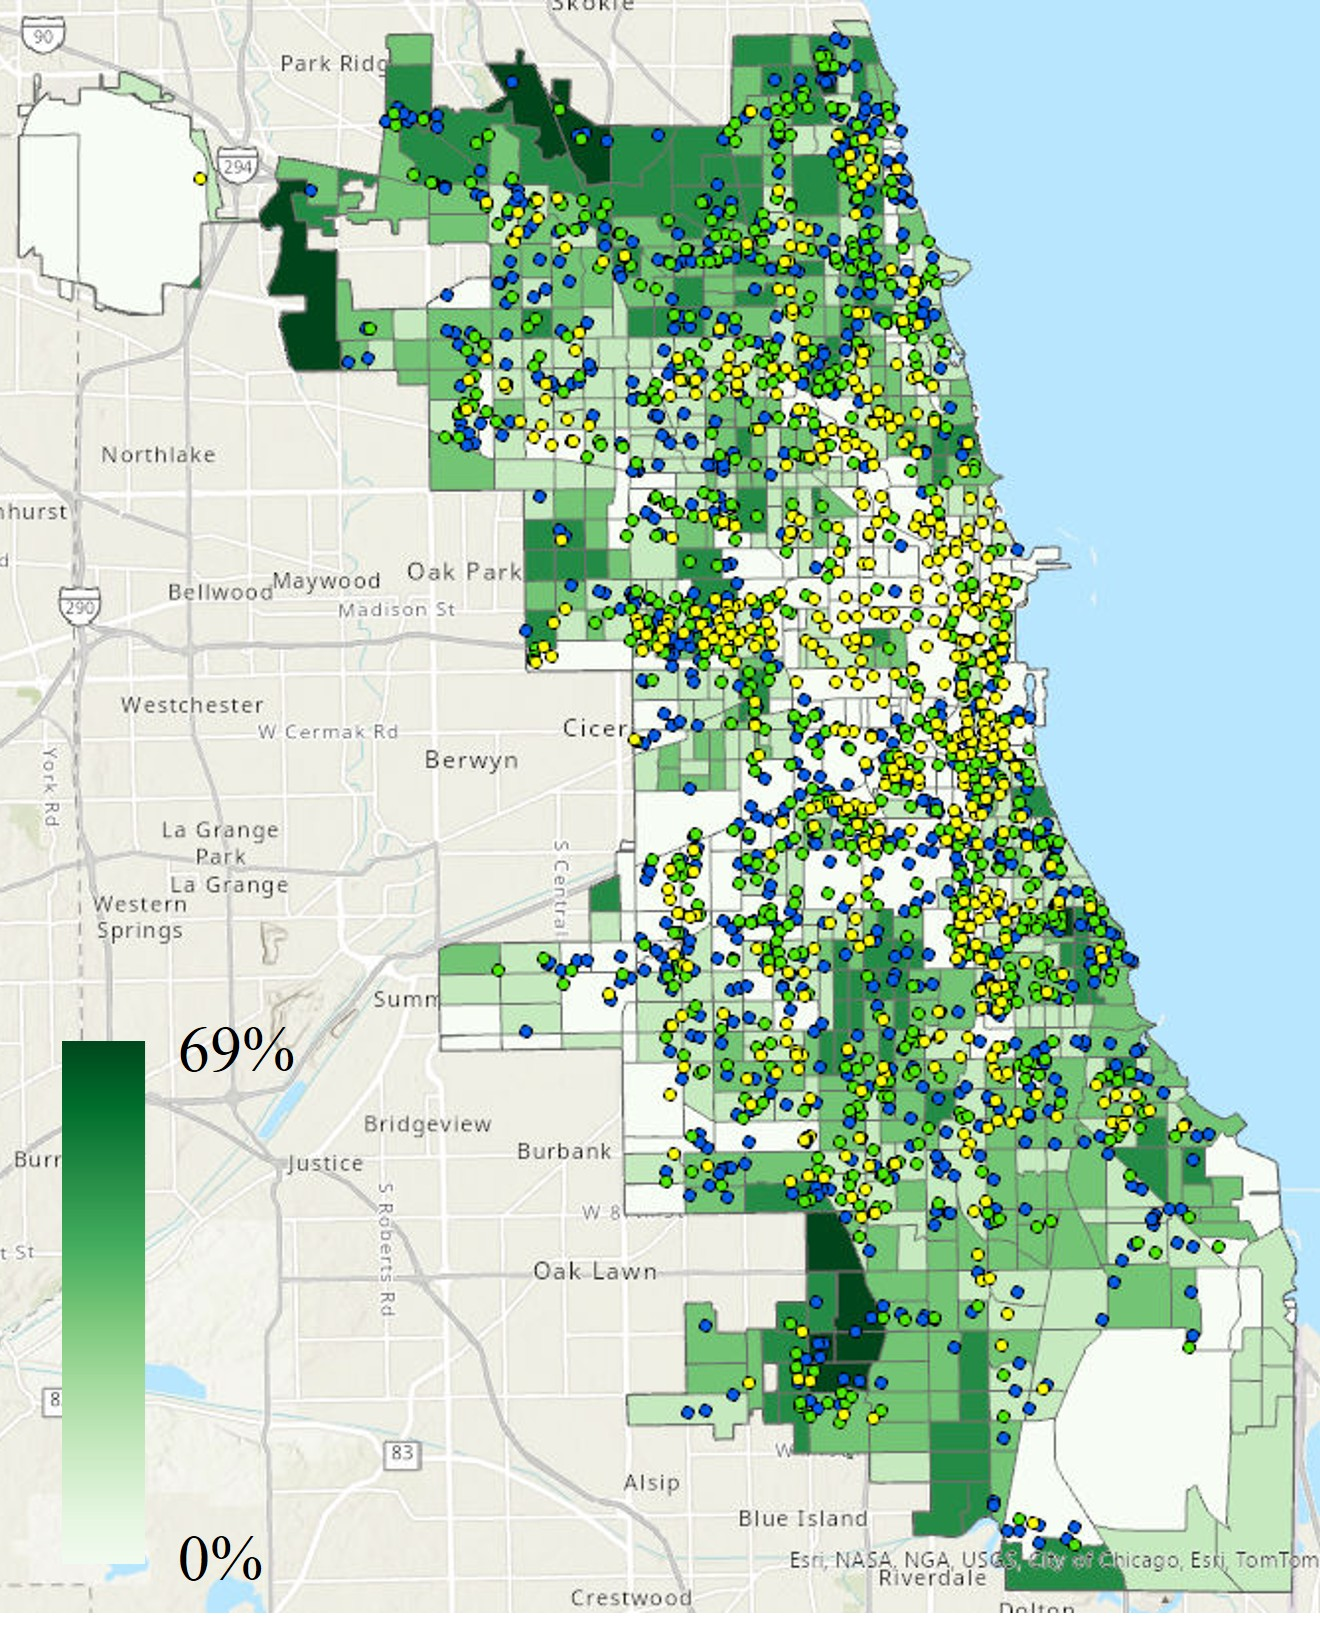
\includegraphics[width=0.25\linewidth]{paper/doc/result_figure/result map_with_vegetation_v4.jpg}}}%
    \qquad
    \hskip -5ex
    \subfloat[\centering]{{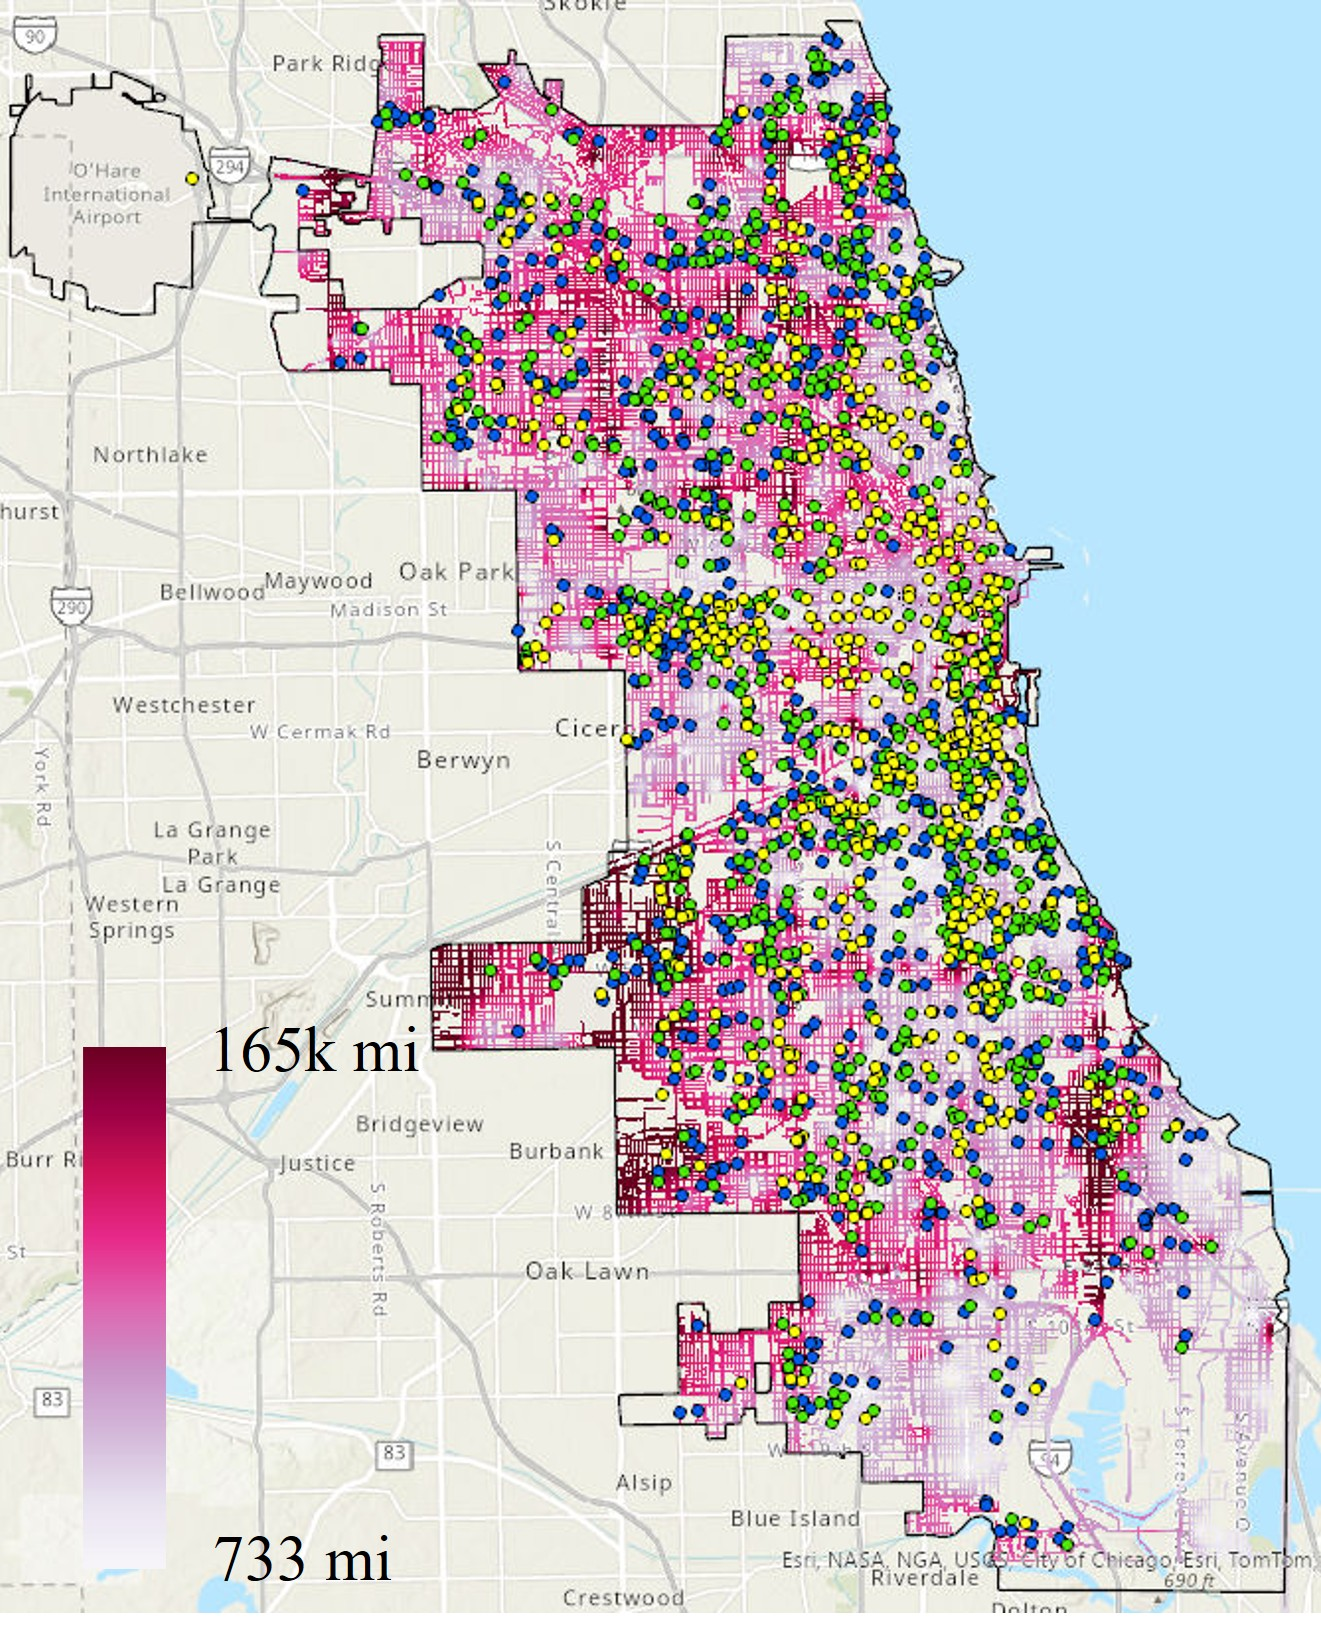
\includegraphics[width=0.25\linewidth]{paper/doc/result_figure/result map_with_traffic flow_v3.jpg}}}%
    \qquad
    \hskip -5ex
    \subfloat[\centering]{{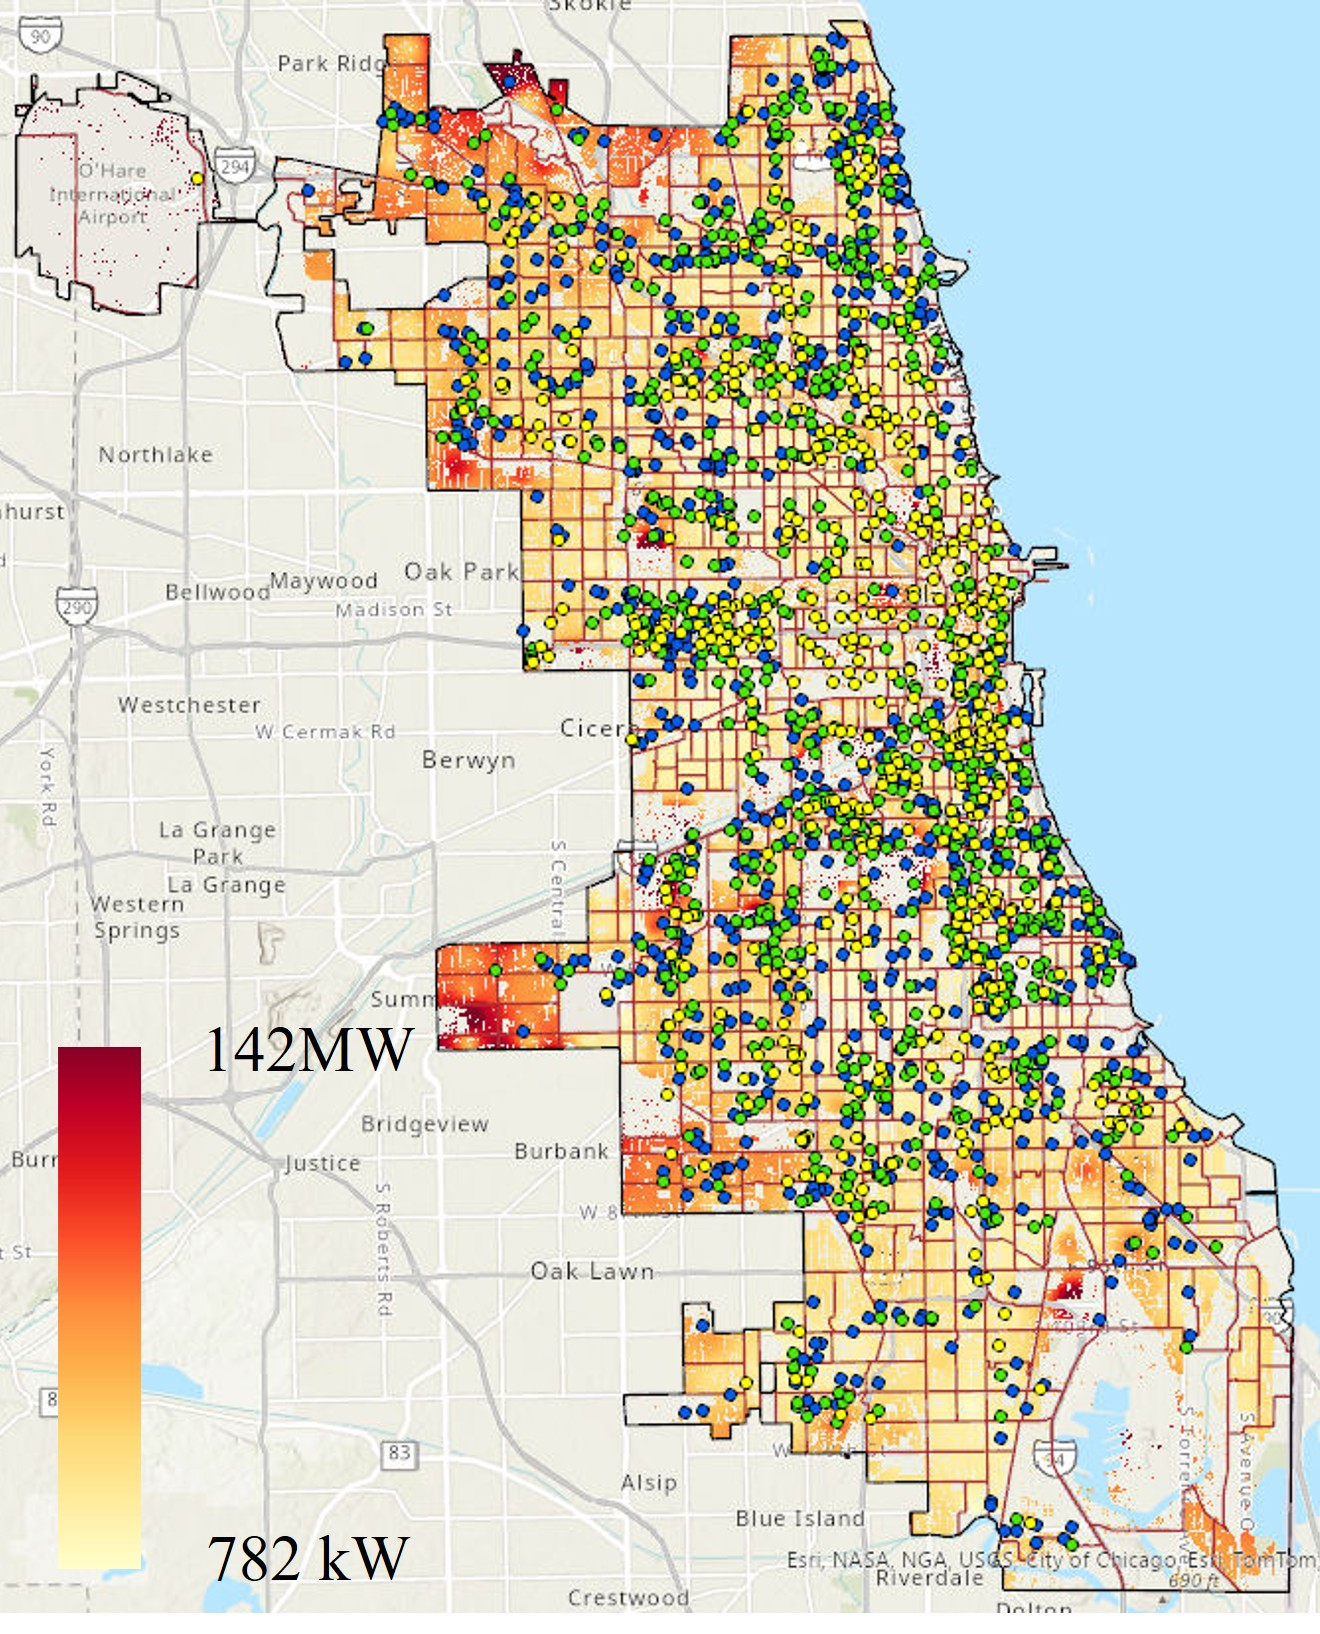
\includegraphics[width=0.25\linewidth]{paper/doc/result_figure/result map_with_solar_v3.jpg}}}%
    
    \captionsetup{format=plain, font=small, labelfont=bf}
    \caption{Potential EVFCS locations of (a) overlapping queried results and alongside (b) vegetation, (c) VMT, and (d) potential solar power}
    \label{fig:peloqr}
\end{figure}

Overall, the potential sites show a tendency to concentrate in the downtown (east central region in Chicago) while gradually spreading toward the outskirts of town. As the query threshold increases (from 6 to 10), the number of selected locations in peripheral areas decreases. To better understand this pattern, we compare the queried results with spatial indicators such as vegetation (\textcolor{red}{Figure \ref{fig:peloqr}}-(b)), VMT (\textcolor{red}{Figure \ref{fig:peloqr}}-(c)), and potential solar power output (\textcolor{red}{Figure \ref{fig:peloqr}}-(d)). \textcolor{red}{Figure \ref{fig:peloqr}}-(b) shows that high-reward EVFCS placements actively avoid zones with dense vegetation, predominantly located in peripheral areas (e.g., north side and west-south side regions). In particular, the highest performance-based allocation strategy (i.e., average reward > 10) is noticeably absent from high vegetation density regions (indicated in dark green). Additionally, \textcolor{red}{Figure \ref{fig:peloqr}}-(c) reveals a strong correlation between EVFCS placement and areas with high charging demand, which tend to align with the road network and dense urban activity. Conversely, \textcolor{red}{Figure \ref{fig:peloqr}}-(d) represents that the EVFCS placement strategy is less influenced by solar potential. This may be because charging demands can still be met via access to the existing transmission network (red polylines in \textcolor{red}{Figure \ref{fig:peloqr}}-(d)), even in regions with limited solar energy potential. 

\section{Discussions}
The optimal allocation of EVFCS is significantly influenced by multiple criteria embedded within the geospatial characteristics of the urban environment. This study proposes MORL models that sequentially make optimal decisions regarding equitable EVFCS placement while simultaneously estimating station sizing. The proposed MORL framework addresses the scalability challenges observed in previous EVCS planning studies by incorporating three elements: multi-objective optimization, geospatial analysis, and a sequential decision-making-based site selection strategy. Traditional approaches, such as MCDM with geospatial analysis, are often limited in subjective weighting methods and no universal function that cannot present generalizable VCS placement model. Also, multi-objective optimization-based EVCS allocation model are inherently restricted in their ability to comprehensively explore the urban environments due to the node-based data format. 

In contrast, the proposed multi-objective optimal decision-making with geospatial analysis approach is capable of investigating optimal EVFCS placement across the entire urban area by learning strategies from capturing the dynamics of relevant geospatial features, as shown in \textcolor{red}{Figure}\ref{fig:peloqr}. The results (\textcolor{red}{Figure}\ref{fig:lpdts}) demonstrate that the model can improve the ability to identify the optimal sites for EVFCS in which all objectives are optimized.

This study presents and evaluates two MORL-based DRL algorithms (1) a single policy multi-objective PPO and () a multi-policies asynchronous federated learning algorithm. While both methods achieve effective allocation strategies, the single-policy MORL (\textcolor{red}{Figure \ref{fig:trlgsmorl}}-(a)) slightly outperforms the federated model in terms of learning stability and resilience against noisy rewards (i.e., sparse rewards). Although the federated multi-policies PPO benefits from the independent optimization of three objectives, it faces challenges due to objective heterogeneity that makes it difficult to aggregate distinct features from policies effectively, which may vanish important features in combining. In contrast, the single policy MORL employs a linear weighted Q-function to optimize the shared advantage function, thereby including all objectives' features in the optimization of the gradient. 

To validate the proposed model's effectiveness, we compared the proposed EVFCS placements (\textcolor{red}{Figure}\ref{fig:cep}-(a) and existing charging infrastructures in Chicago; level-2 (\textcolor{red}{Figure}\ref{fig:cep}-(b)) and direct current (DC) fast ((\textcolor{red}{Figure}\ref{fig:cep}-(c)). 

\begin{figure}[htb]
    \centering
    \subfloat[\centering]{{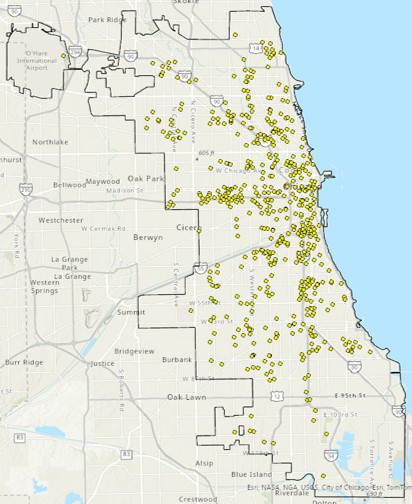
\includegraphics[width=0.27\linewidth]{paper/doc/result_figure/highest_result_v2.jpg}}}%
    \qquad
    \subfloat[\centering]{{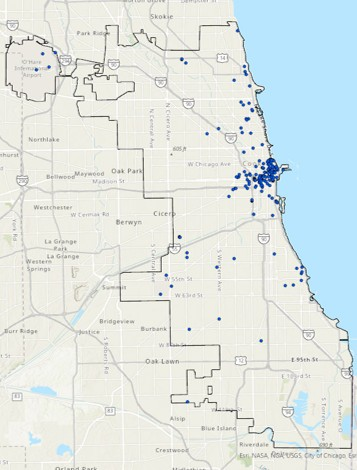
\includegraphics[width=0.27\linewidth]{paper/doc/level2_ExistCS_v1.jpg}}}%
    \qquad
    \subfloat[\centering]{{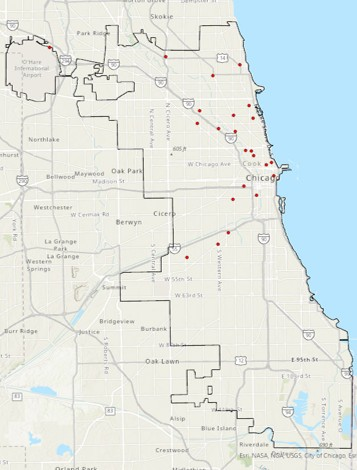
\includegraphics[width=0.27\linewidth]{paper/doc/DCfast_ExistCS_v1.jpg}}}%
    
    \captionsetup{format=plain, font=small, labelfont=bf}
    \caption{Comparison of EVCS placements between (a) proposed allocation plan, (b) existing level-2 EVCS, and (c) existing DC fast EVCS}
    \label{fig:cep}
\end{figure}

While existing stations are heavily clustered around downtown (in east central regions), our model proposes a more equitable spatial distribution, extending installation to underserved regions on the west, south, and north sides. This expansion enhances charging accessibility in marginalized communities across Chicago (Carlton and Sultana 2022) \cite{Carlton2022}. Furthermore, when compared with racial demographic distributions (Bharagava et al. 2024) \cite{Bhargava2024}, the proposed model proposes to improve equity by expanding the placement of EVFCSs to areas with a high proportion of minority populations (south and west central regions). 

Nevertheless, two regions remain unallocated: the northwest (including international airport) (\textcolor{red}{Figure}\ref{fig:urns}-(a) and the southeast (characterized by nature areas) (\textcolor{red}{Figure}\ref{fig:urns}-(b)). 

\begin{figure}[h]
    \centering
    \subfloat[\centering]{{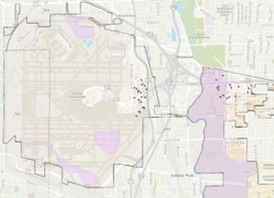
\includegraphics[width=0.4\linewidth]{paper/doc/northwest_v1.jpg}}}%
    \qquad
    \subfloat[\centering]{{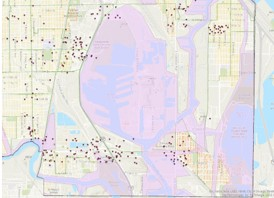
\includegraphics[width=0.4\linewidth]{paper/doc/southeast_v1.jpg}}}%

    \captionsetup{format=plain, font=small, labelfont=bf}
    \caption{Unallocation regions of (a) northwest (international airport), and (b) southeast (vegetation)}
    \label{fig:urns}
\end{figure}

These areas were excluded because they failed to meet one or more of the objectives. The northwest region lacks sufficient charging demand, energy resources, and urban infrastructure, while the southeast poses environmental concerns such as nature conservation and unsuitable land use. To expand the charging accessibility, these zones may still be viable for lower-level (e.g., Level 2) or federally subsidized charging stations that do not require all objectives to be met. 

\vspace{0.5cm}

Future research should address the following limitations. First, although the proposed model can be built with a static daily dataset, such as VMT and solar energy generation from rooftops, further investigation is needed to consider time-series datasets to capture dynamic interactions between EVFCS usage and the power grid for the reliability of the distribution network. Second, this study assumes full rooftop solar panel deployment and complete energy availability for EVFCS operation, which may not reflect realistic energy constraints. To overcome these limitations, future research should integrate power system operation constraints to jointly optimize energy distribution and charging infrastructure planning, ensuring long-term system reliability and equity in EVFCS deployment.  

\section{Conclusion}
The current public fast-charging infrastructure is highly skewed, with deployments concentrated primarily in high-demand areas such as downtown districts. This pattern exacerbates spatial disparities in access to charging services and limits equitable opportunities for electric vehicle (EV) users across urban areas. While recent studies have attempted to allocate EV charging stations with distributed energy resources (DERs), existing methods face challenges in scalability and generalizability. These methods are often restricted to district-level applications, constrained by the graph-structured data format, or limited to evaluating pre-selected candidate sites. 

To address these limitations, this study proposes a multi-objective sequential decision-making framework for the optimal allocation of electric vehicle fast charging stations (EVFCS), powered by solar energy. The approach combines geospatial analysis with deep reinforcement learning (DRL) to enable dynamic and adaptive exploration of optimal charging station placements. Specifically, this study optimizes multiple objectives, minimizing environmental degradation and maximizing economic profitability and urban accessibility, by learning and recognizing critical geospatial features in the urban areas. The two-phase site selection strategy, based on kernel density-based distribution probability, enables equitable allocation of EVFCS throughout urban areas while ensuring that all objectives are satisfied. Applied to the city of Chicago, the model achieved an average reward of 7.5 (\textcolor{red}{Figure}\ref{fig:trlgsmorl}-(a), indicating its ability to identify optimal locations even in previously unseen areas. The model successfully proposes the placement of fast charging stations in urban areas that can be spread out across the urban landscape, even into underserved areas (\textcolor{red}{Figure}\ref{fig:cep}-(a), where all objectives are jointly optimized. The major findings and implications of this study are summarized as follows: (1) The proposed multi-objective DRL model enables effective exploration and optimization in complex, unseen geospatial environments by learning map-based features, (2) The model can be resilient and stable learning that can less impact on the sparse rewards (\textcolor{red}{Figure}\ref{fig:trlgsmorl}), (3) The two-stage site selection strategy ensures an equitable allocation of charging infrastructure city-wide (\textcolor{red}{Figure}\ref{fig:lpdts}), and (4) The allocated potential charging infrastructure is strongly affected by the envrionemntal, economic, and urbanity criteria (\textcolor{red}{Figure}\ref{fig:peloqr}).

Overall, this study provides a scalable and adaptable framework for optimizing large-scale EVFCS infrastructure, promoting equitable access to EV charging services. The model offers a holistic solution that considers the needs of multiple stakeholders, including CS operators, EV users, and environmental advocates, thereby contributing to the broader goal of urban sustainability. Despite its strengths, future work should expand the model to incorporate time-series datasets, including hourly electricity generation, solar energy output, and charging demand patterns, to mitigate potential load spikes caused by new charging infrastructure. Furthermore, additional considerations of equity metrics are recommended to ensure fair and inclusive access to future EVFCS deployment. 

\newpage
%% The Appendices part is started with the command \appendix;
%% appendix sections are then done as normal sections
\appendix
\section{Appendix}
\setcounter{figure}{0}
Here is for the loss graphs for asynchronous federated learning-based MORL: Environment criteria actor loss in (A.1); critic loss in (A.2); entropy loss in (A.3), economic criteria actor loss in (A.4); critic loss in (A.5); entropy loss in (A.6), and urbanity criteria actor loss in (A.7); critic loss in (A.8); entropy loss in (A.9).

\begin{figure}[h!]
    \centering
    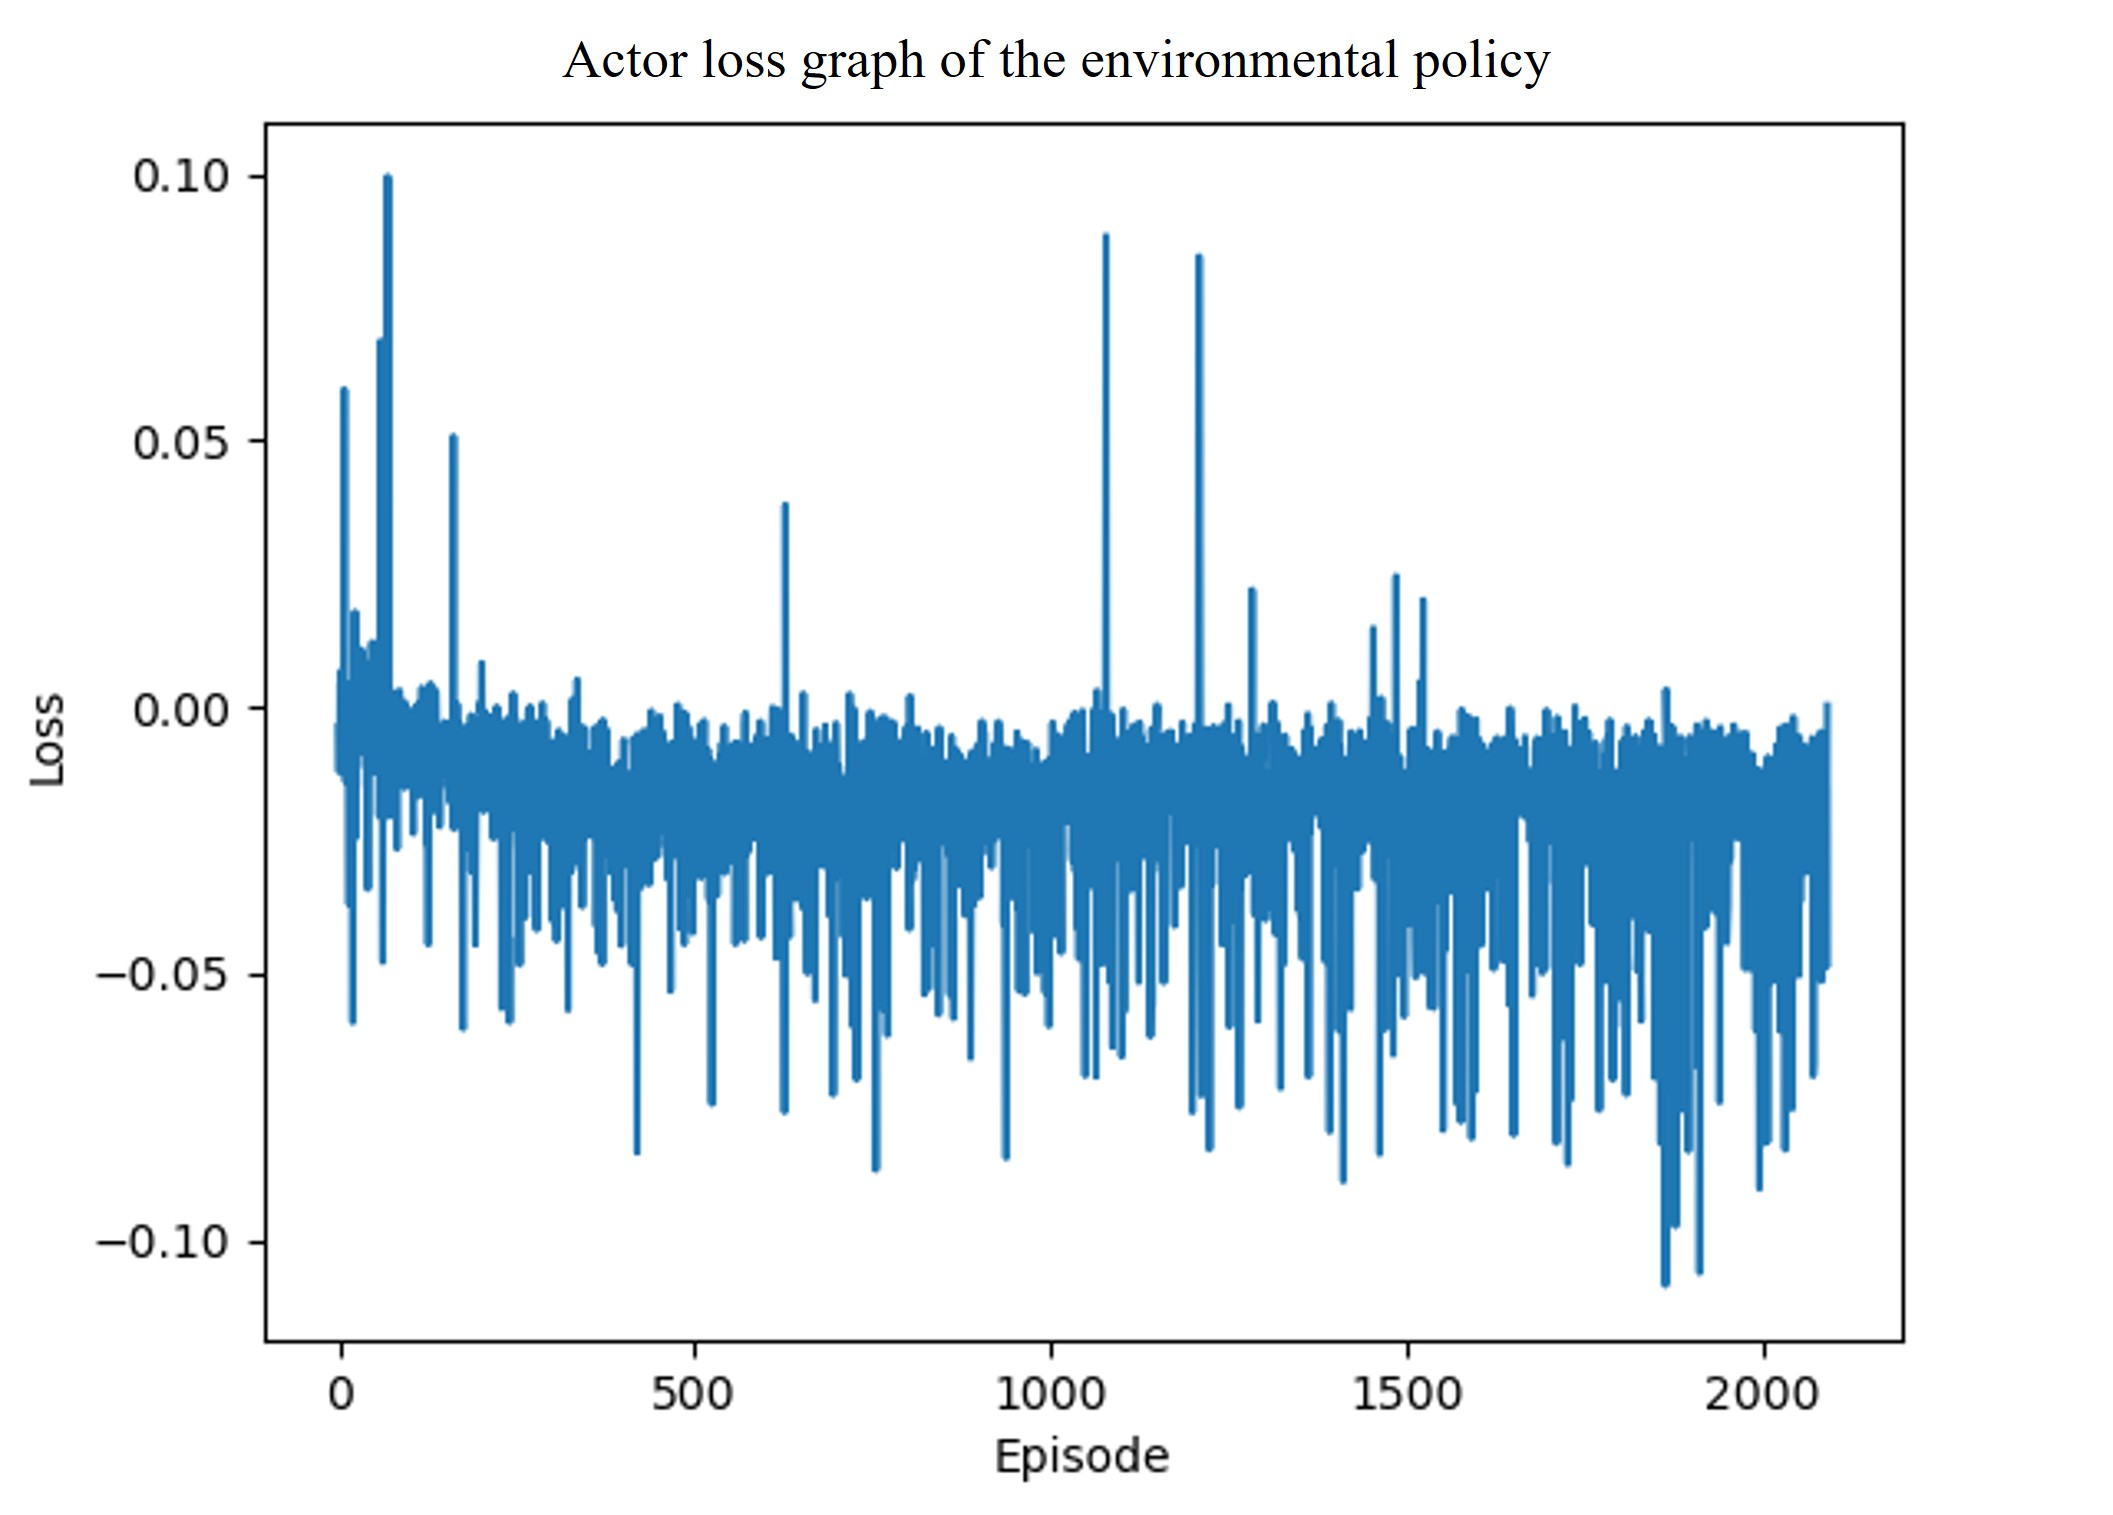
\includegraphics[width=0.7\linewidth]{paper/doc/result_figure/AFMORL_env_ac_loss_v1.jpg}
    \caption{Actor loss graph of the environmental policy}
    
    \label{fig:enter-label}
\end{figure}

\begin{figure}[h!]
    \centering
    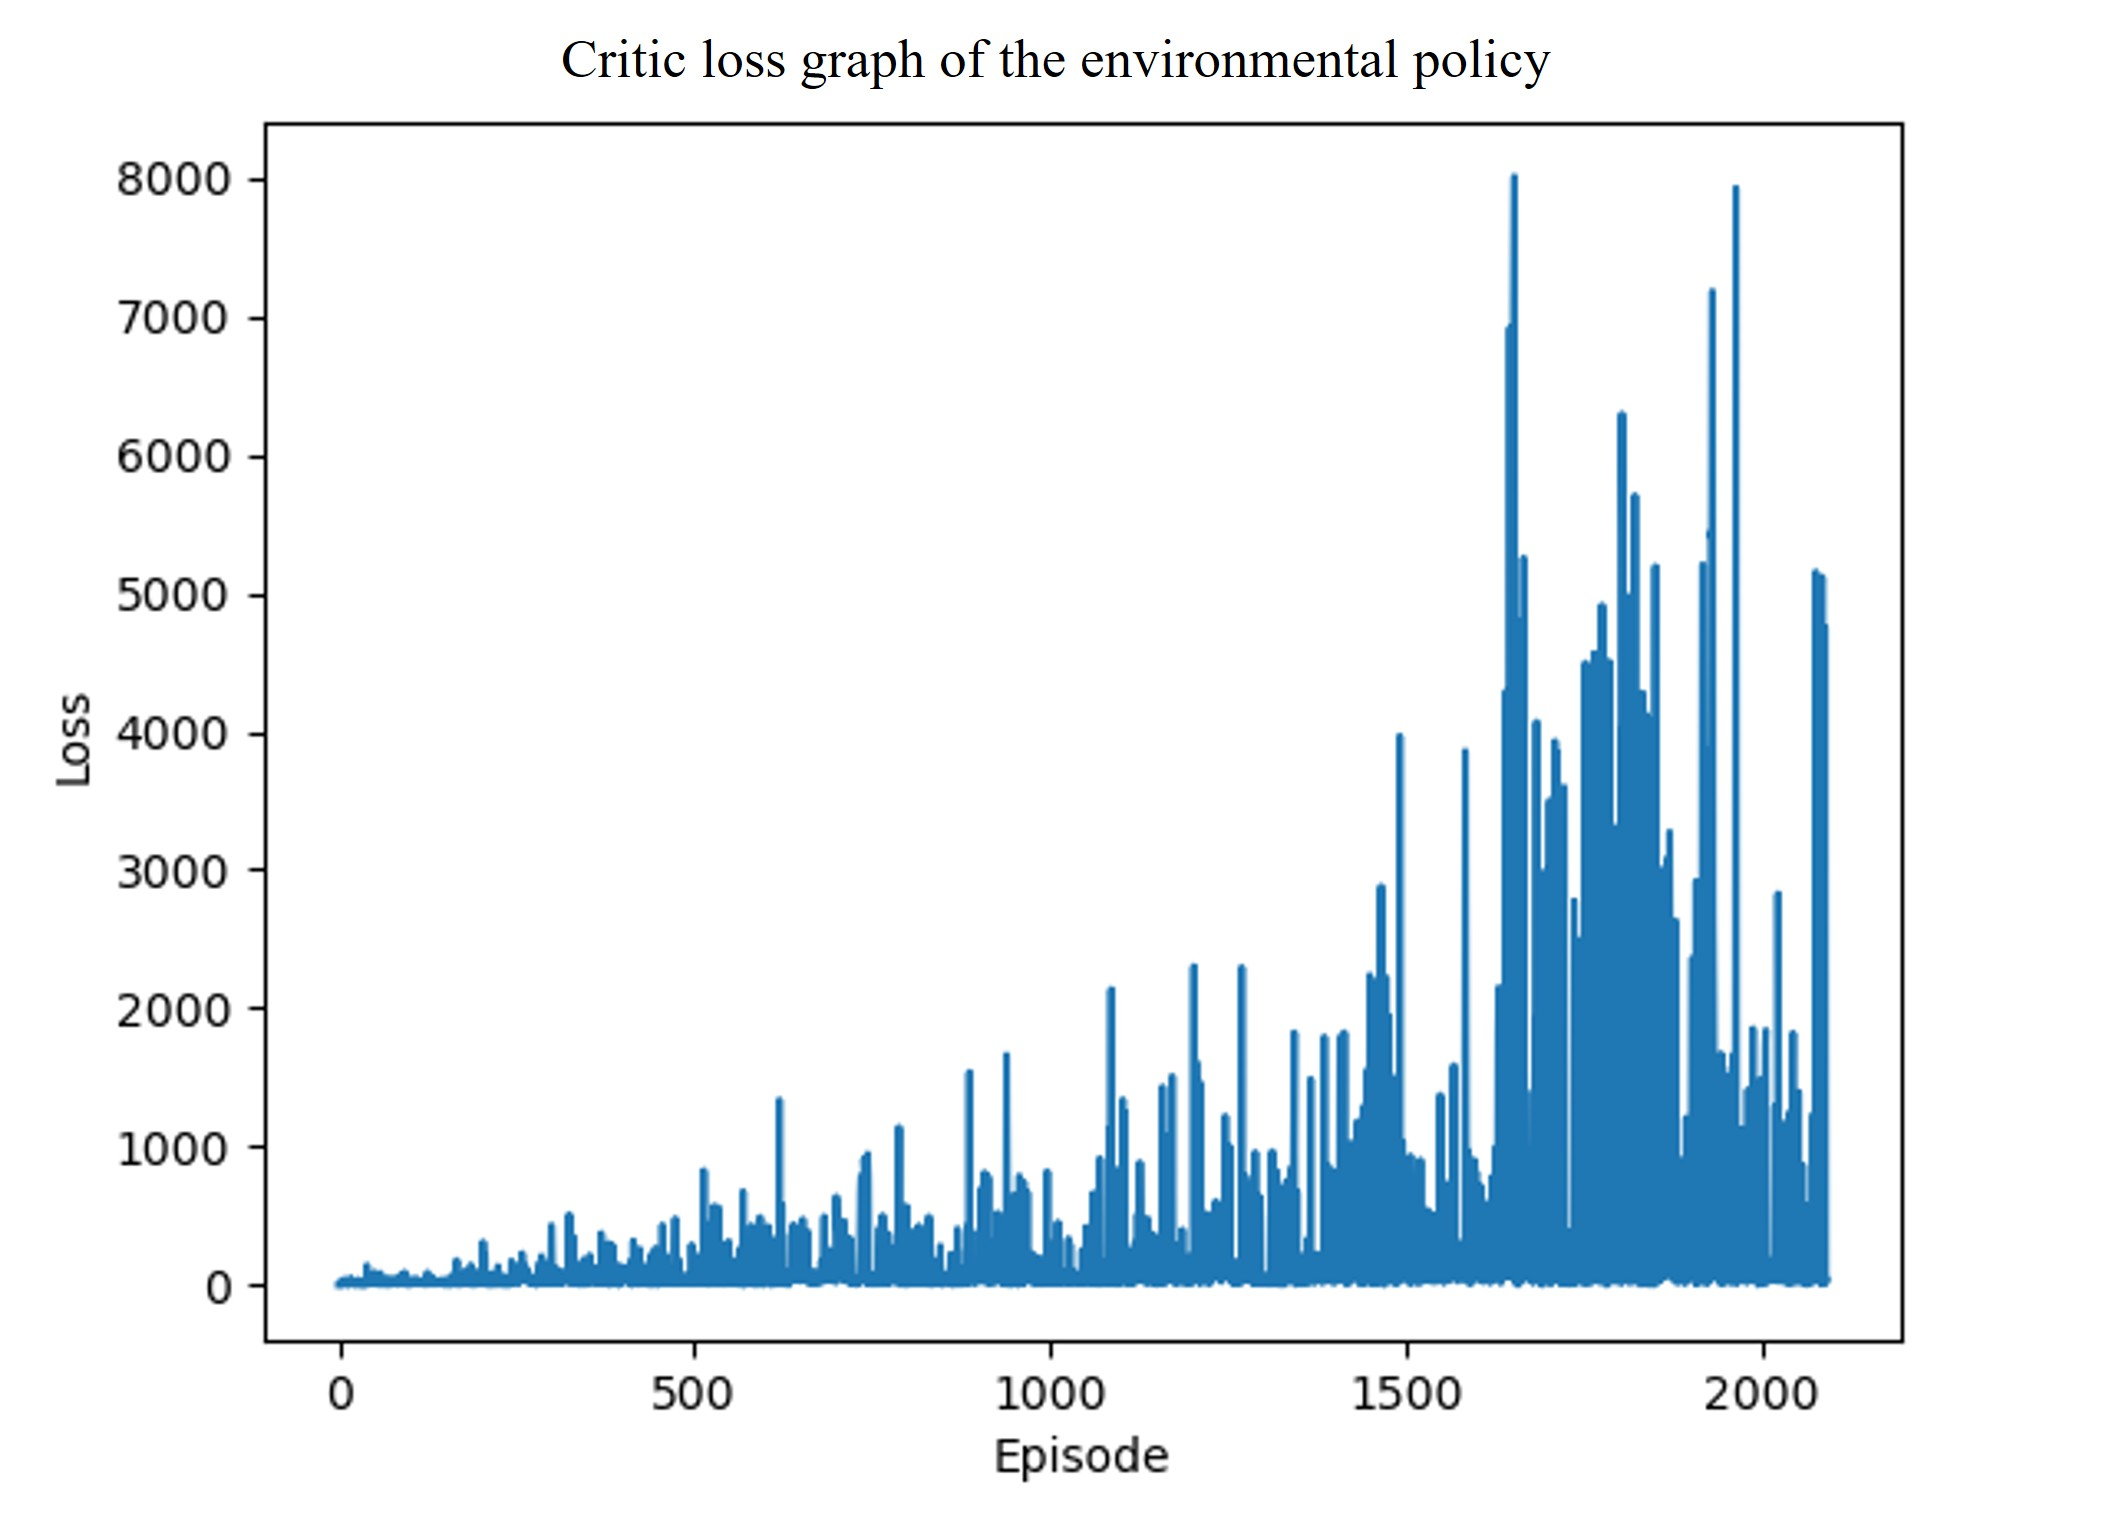
\includegraphics[width=0.7\linewidth]{paper/doc/result_figure/AFMORL_env_cri_loss_v1.jpg}
    \caption{Critic loss graph of the environmental policy}
    
    \label{fig:enter-label}
\end{figure}

\begin{figure}[h!]
    \centering
    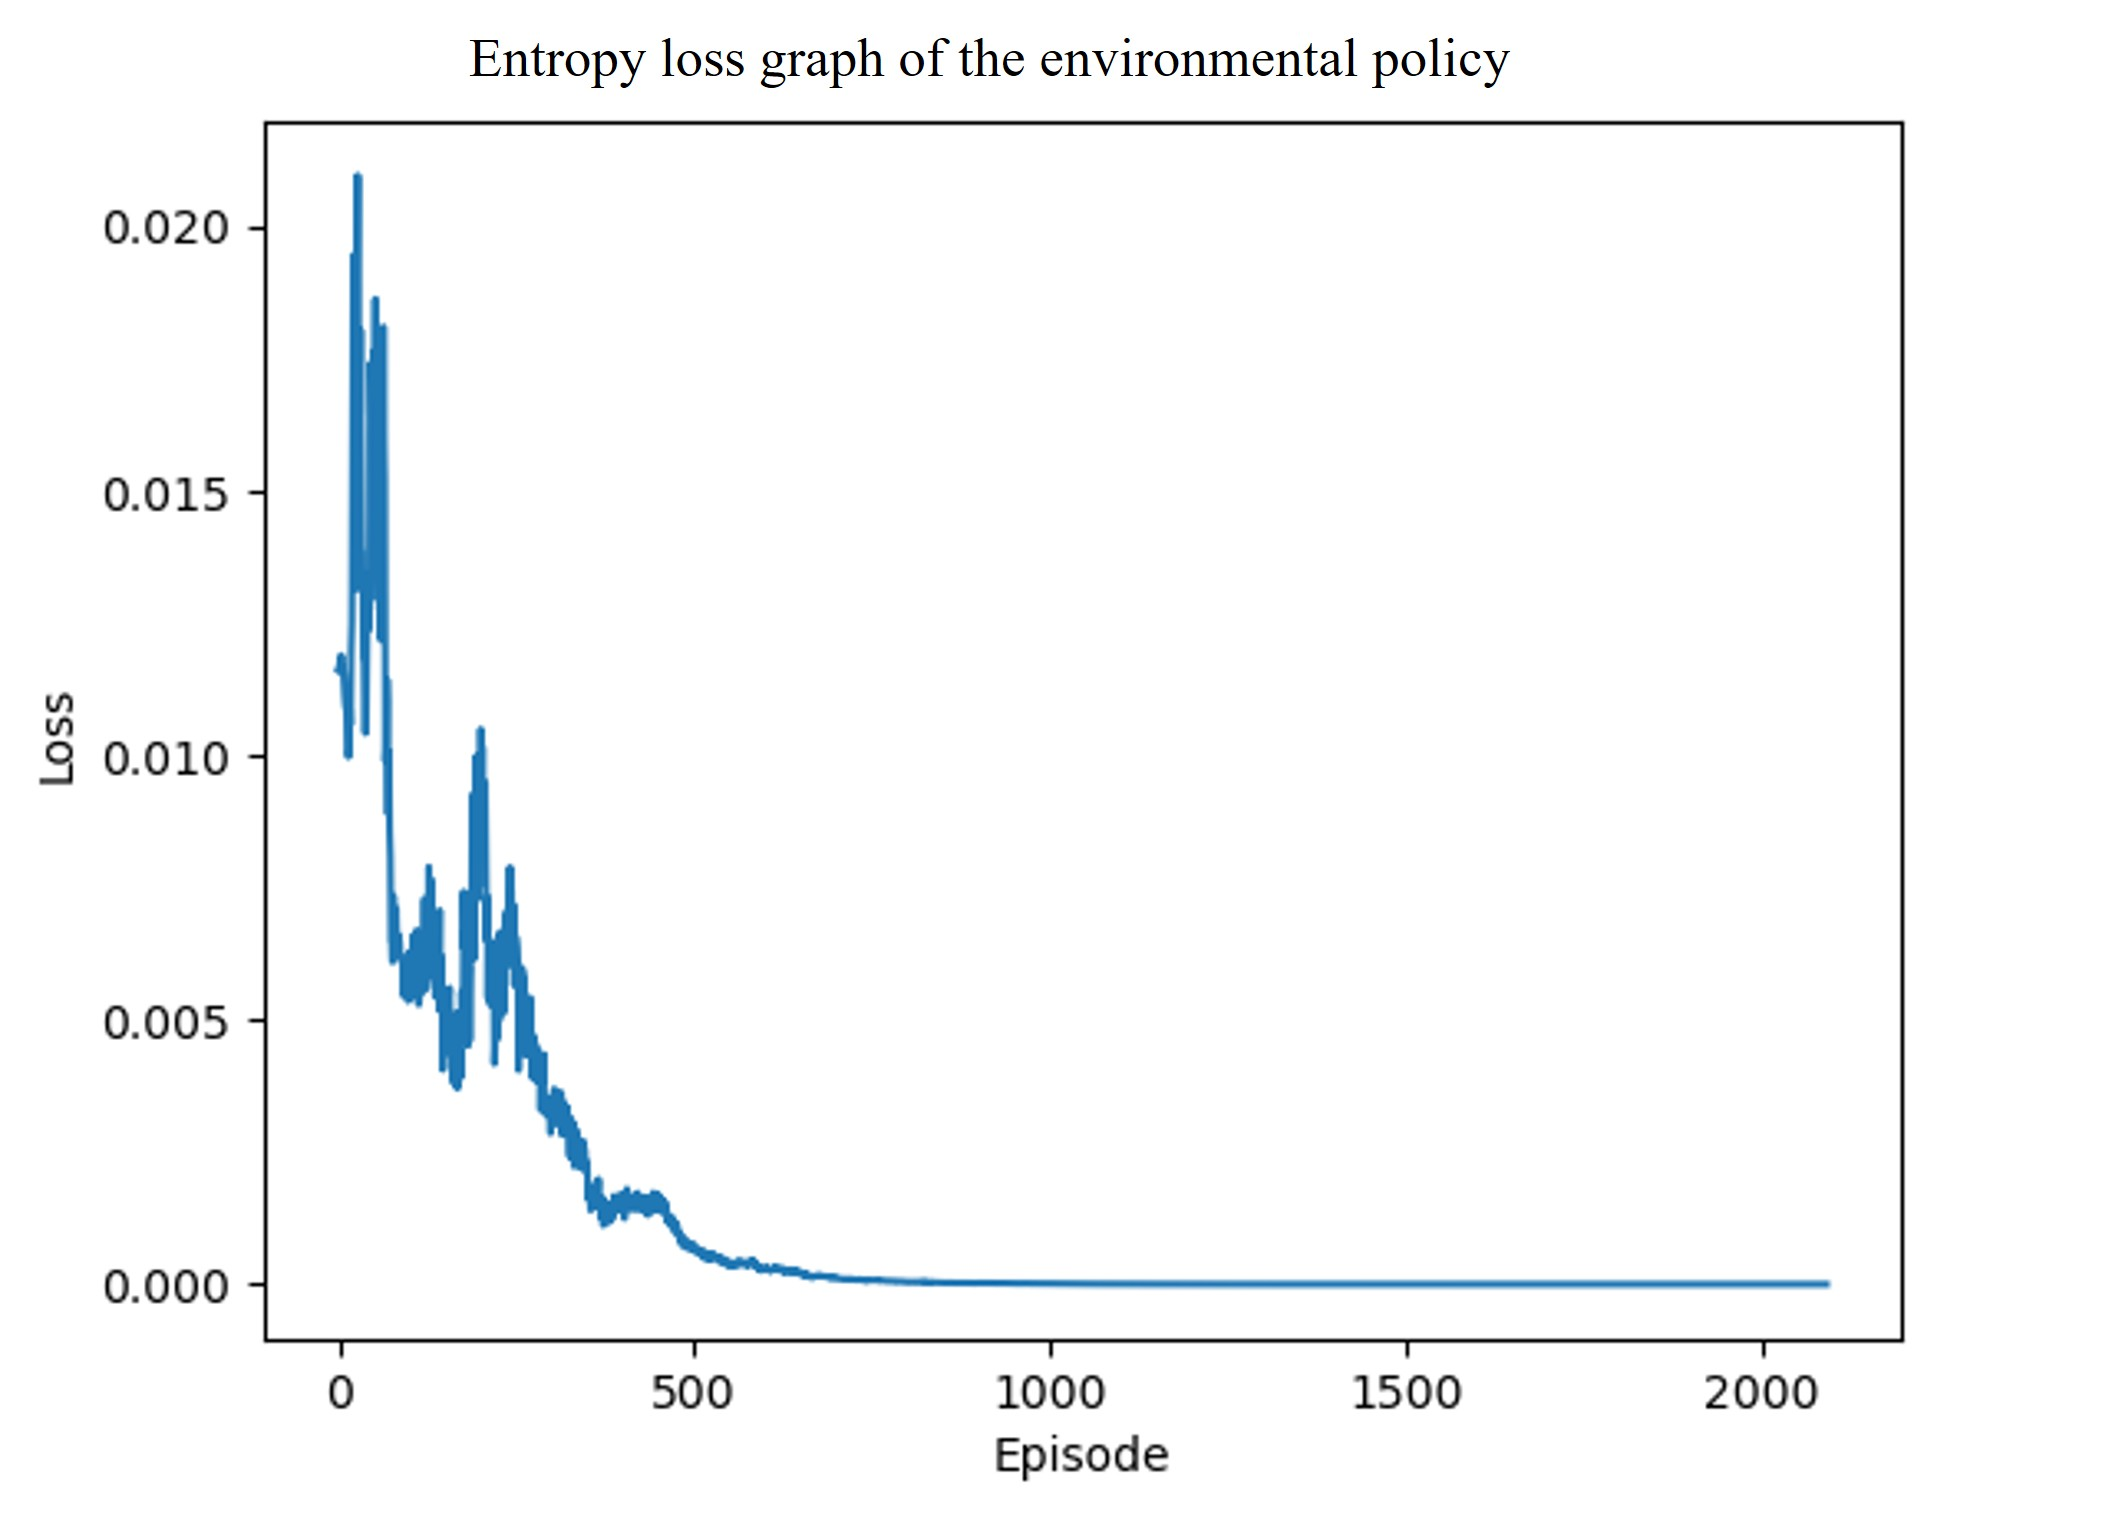
\includegraphics[width=0.7\linewidth]{paper/doc/result_figure/AFMORL_env_entr_loss_v1.jpg}
    \caption{Entropy loss graph of the environmental policy}
    
    \label{fig:enter-label}
\end{figure}

\begin{figure}[h!]
    \centering
    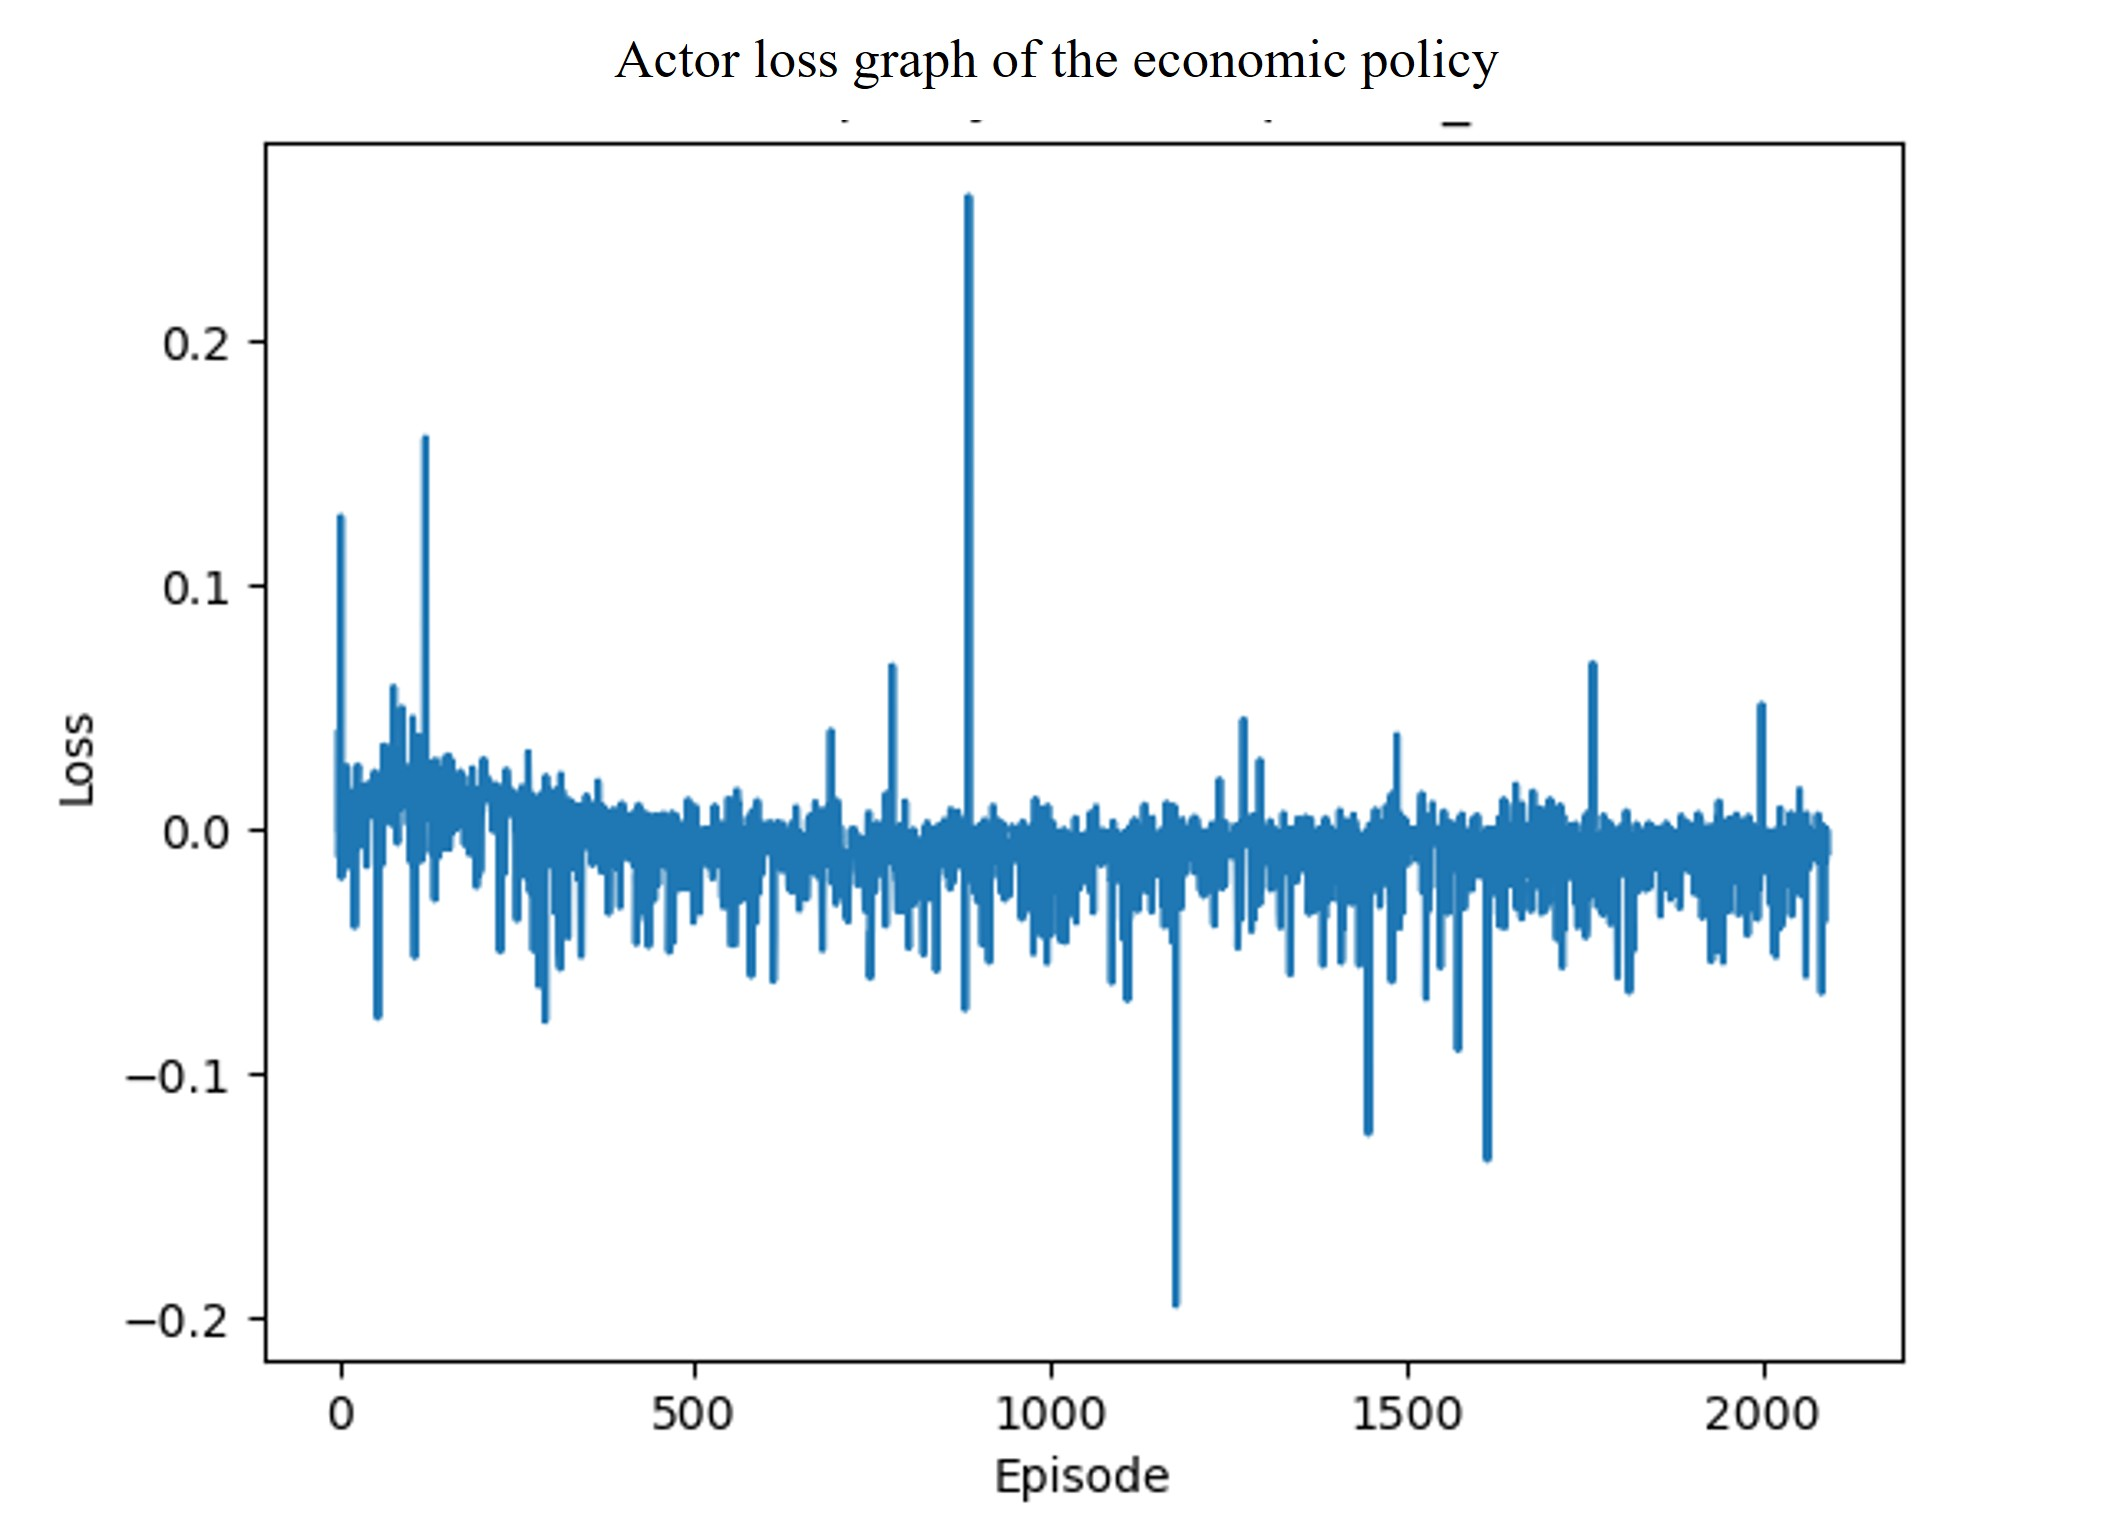
\includegraphics[width=0.7\linewidth]{paper/doc/result_figure/AFMORL_eco_ac_loss_v1.jpg}
    \caption{Actor loss graph of the economic policy}
    
    \label{fig:enter-label}
\end{figure}

\begin{figure}[h!]
    \centering
    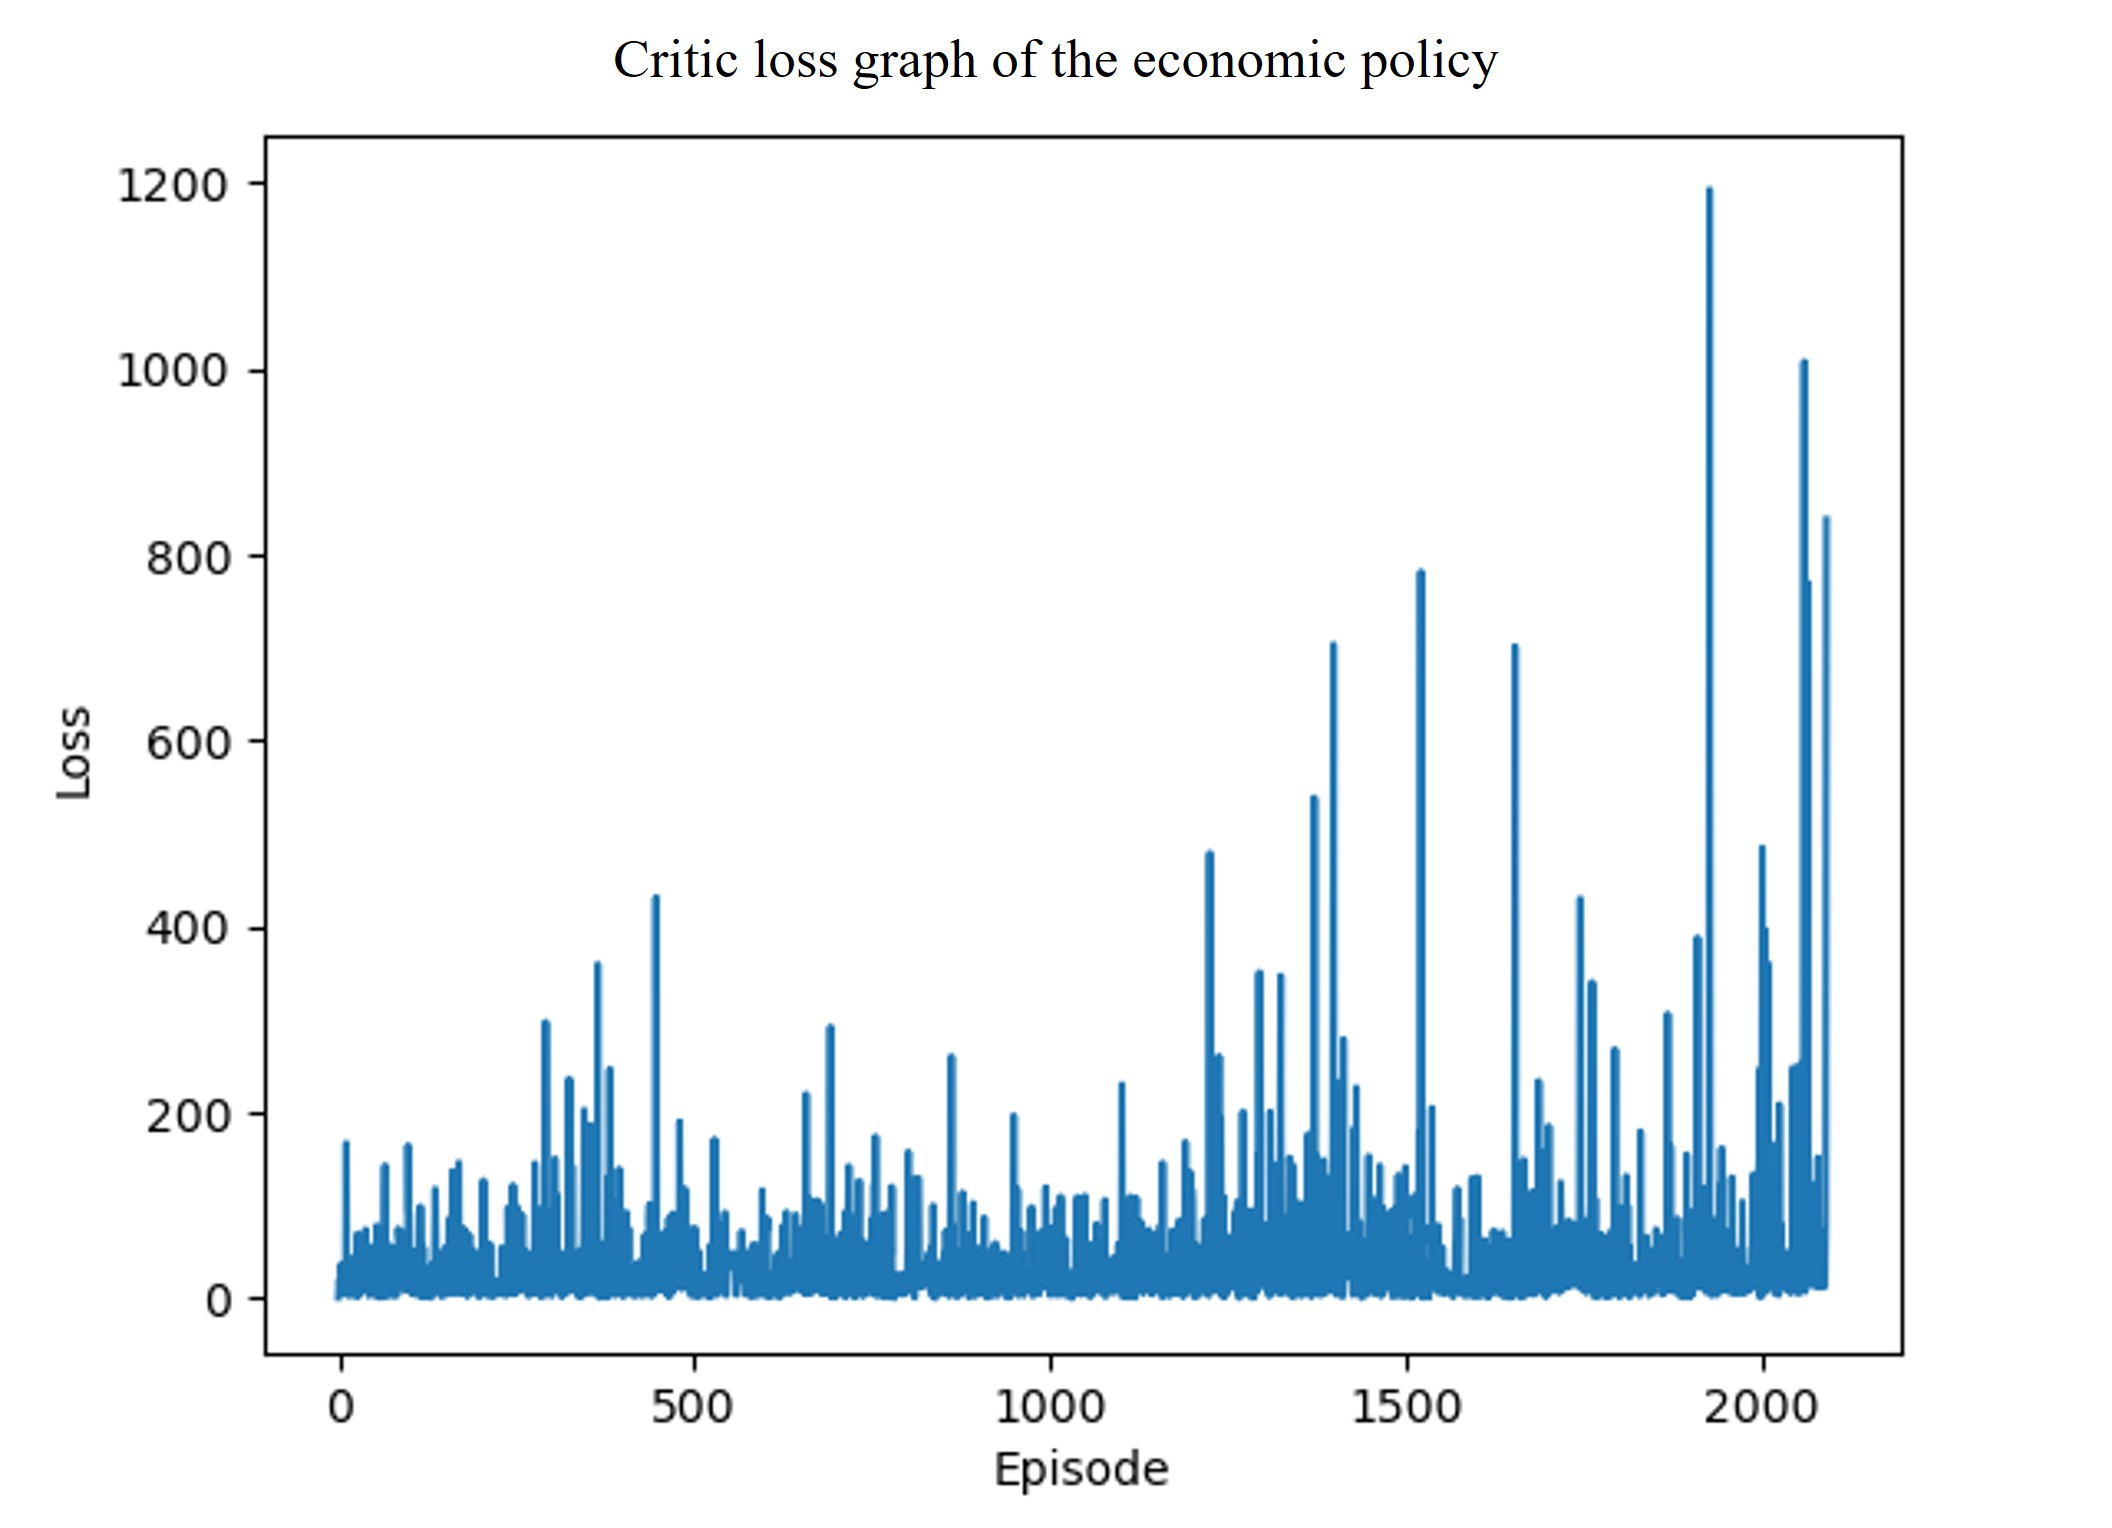
\includegraphics[width=0.7\linewidth]{paper/doc/result_figure/AFMORL_eco_cri_loss_v1.jpg}
    \caption{Critic loss graph of the economic policy}
    
    \label{fig:enter-label}
\end{figure}

\begin{figure}[h!]
    \centering
    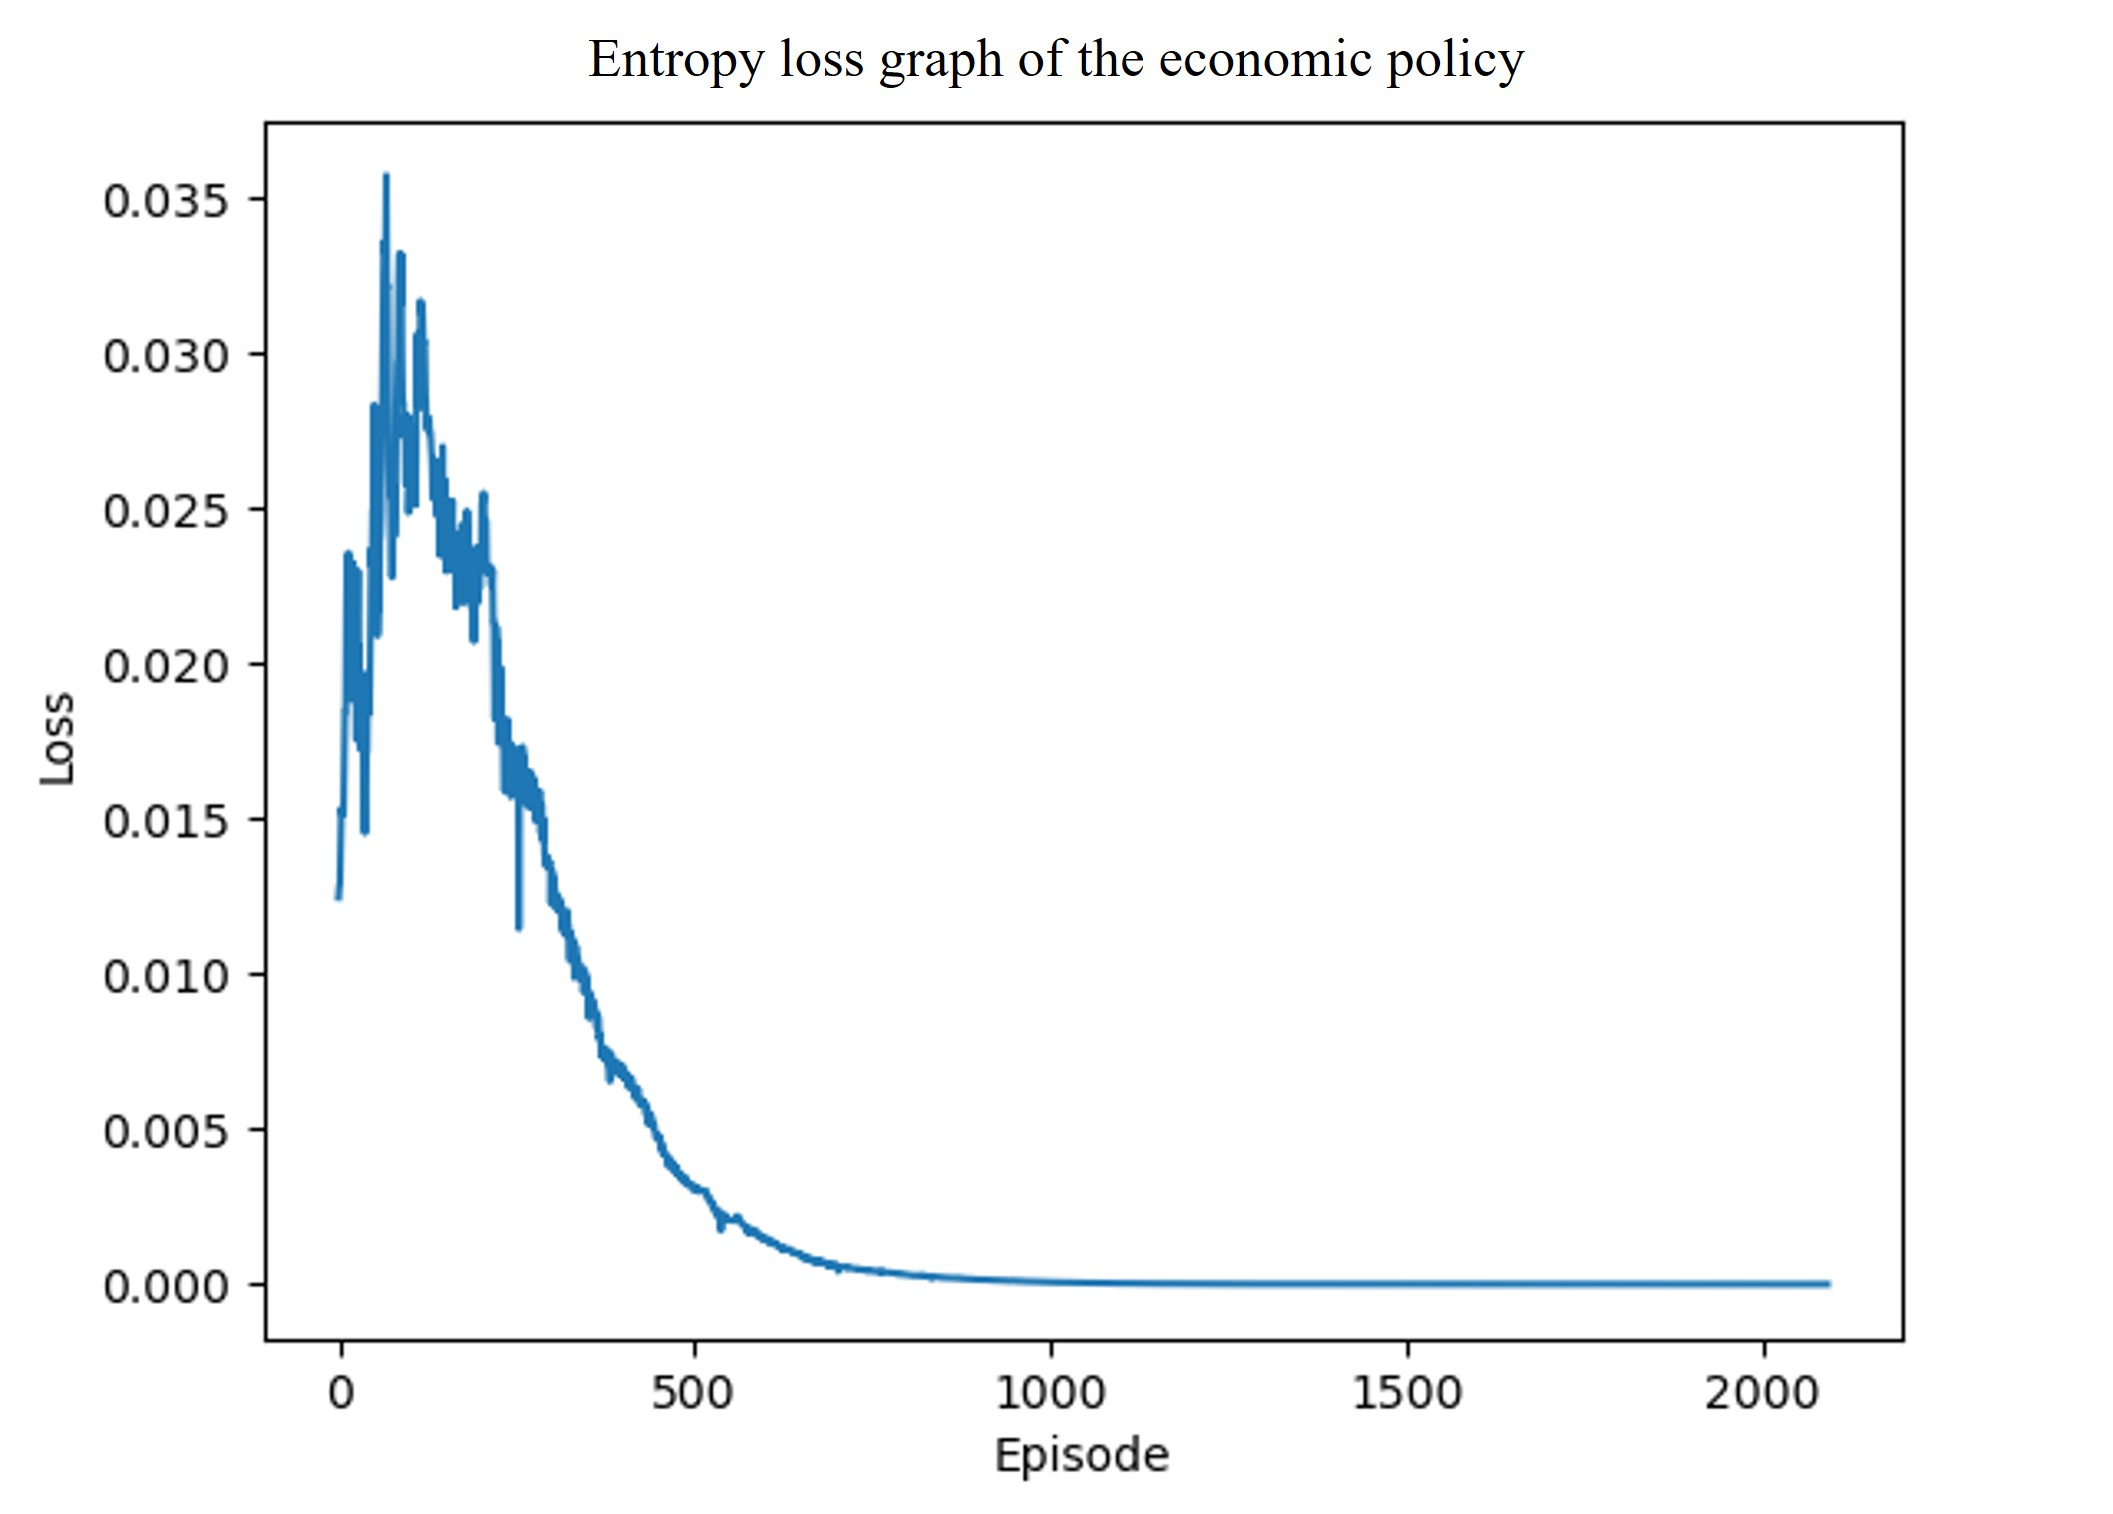
\includegraphics[width=0.7\linewidth]{paper/doc/result_figure/AFMORL_eco_entr_loss_v1.jpg}
    \caption{Entropy loss graph of the economic policy}
    
    \label{fig:enter-label}
\end{figure}

\begin{figure}[h!]
    \centering
    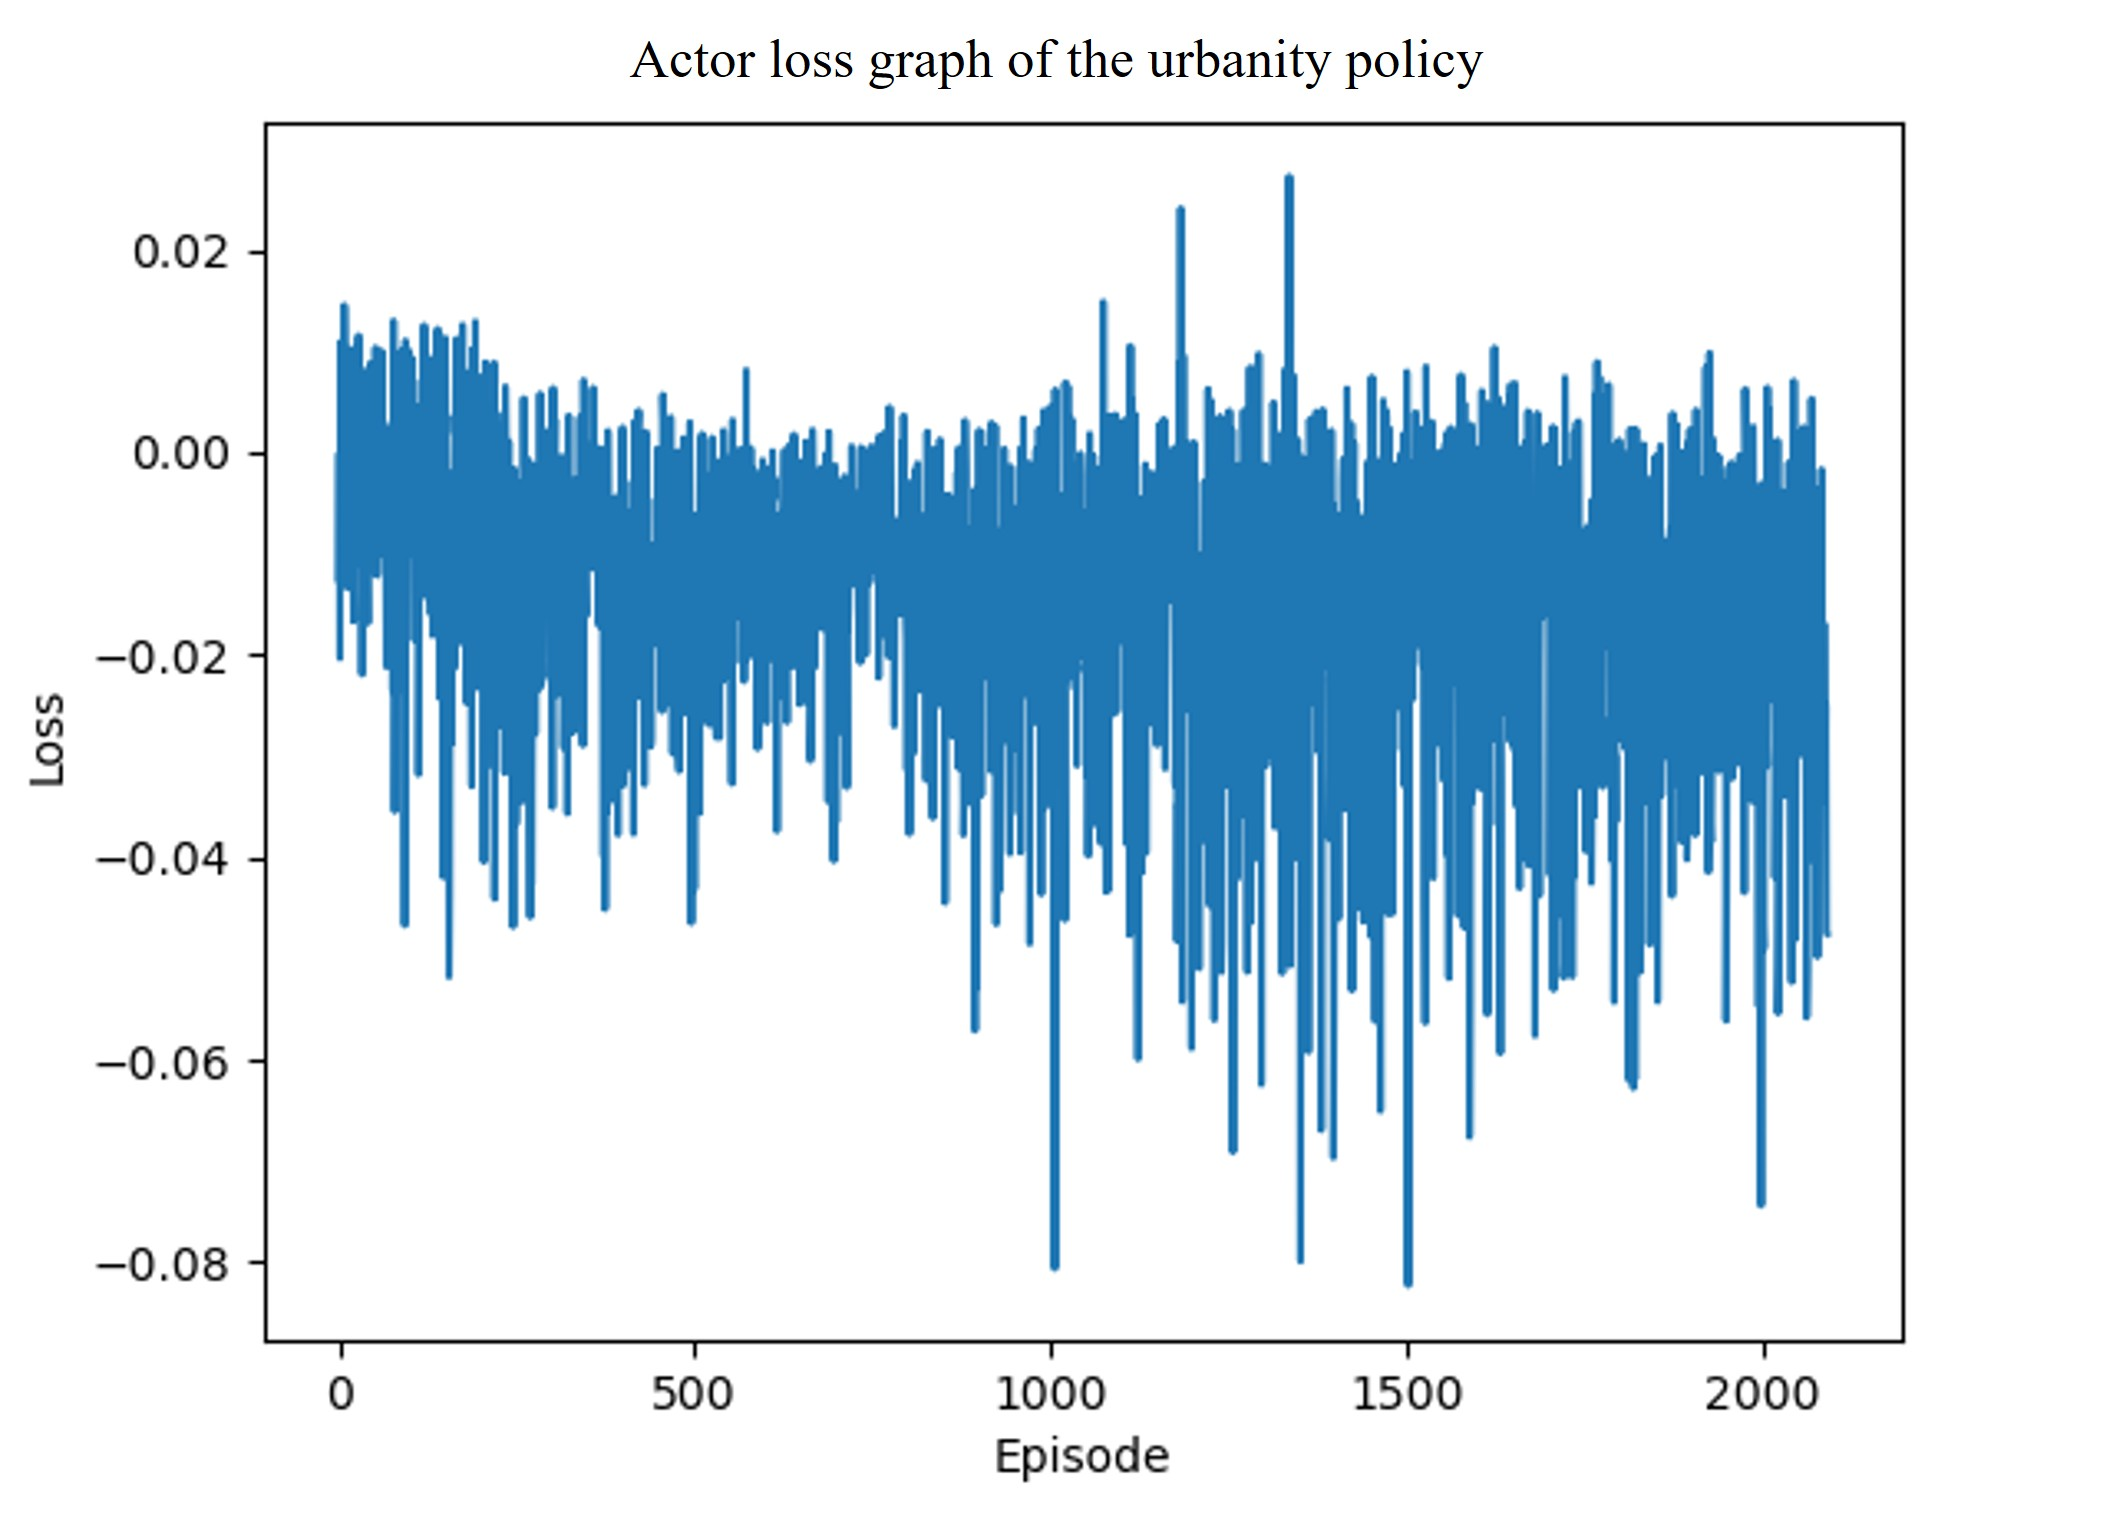
\includegraphics[width=0.7\linewidth]{paper/doc/result_figure/AFMORL_urb_act_loss_v1.jpg}
    \caption{Actor loss graph of the urbanity policy}
    
    \label{fig:enter-label}
\end{figure}

\begin{figure}[h!]
    \centering
    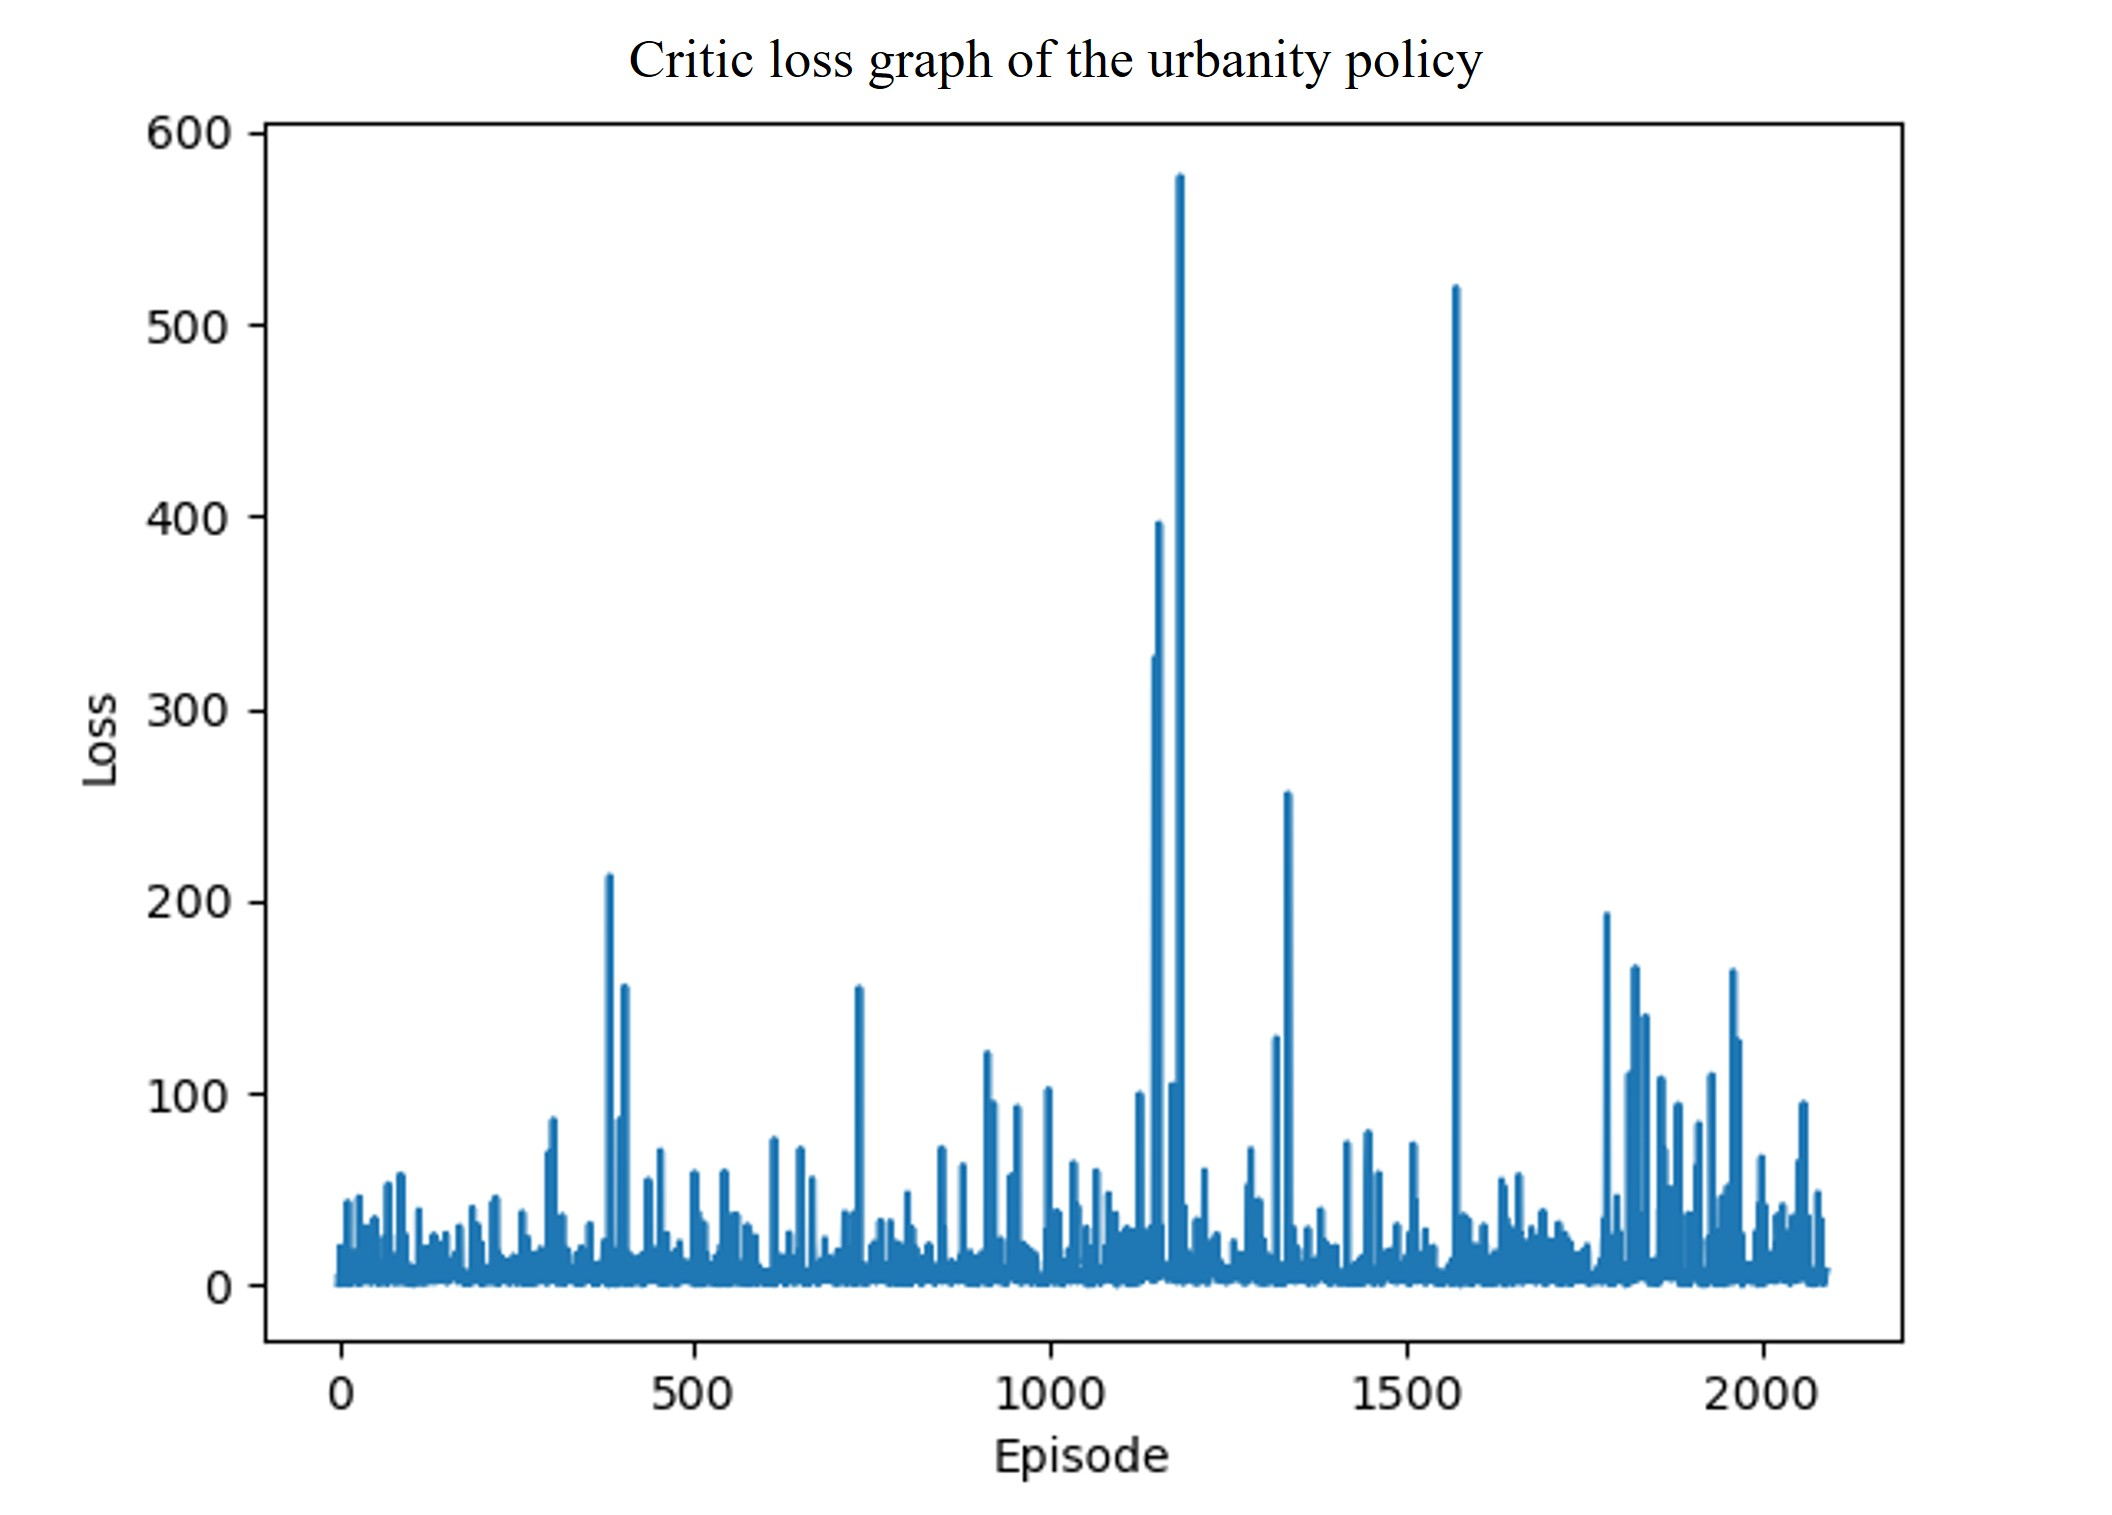
\includegraphics[width=0.7\linewidth]{paper/doc/result_figure/AFMORL_urb_cri_loss_v1.jpg}
    \caption{Critic loss graph of the urbanity policy}
    
    \label{fig:enter-label}
\end{figure}

\begin{figure}[h!]
    \centering
    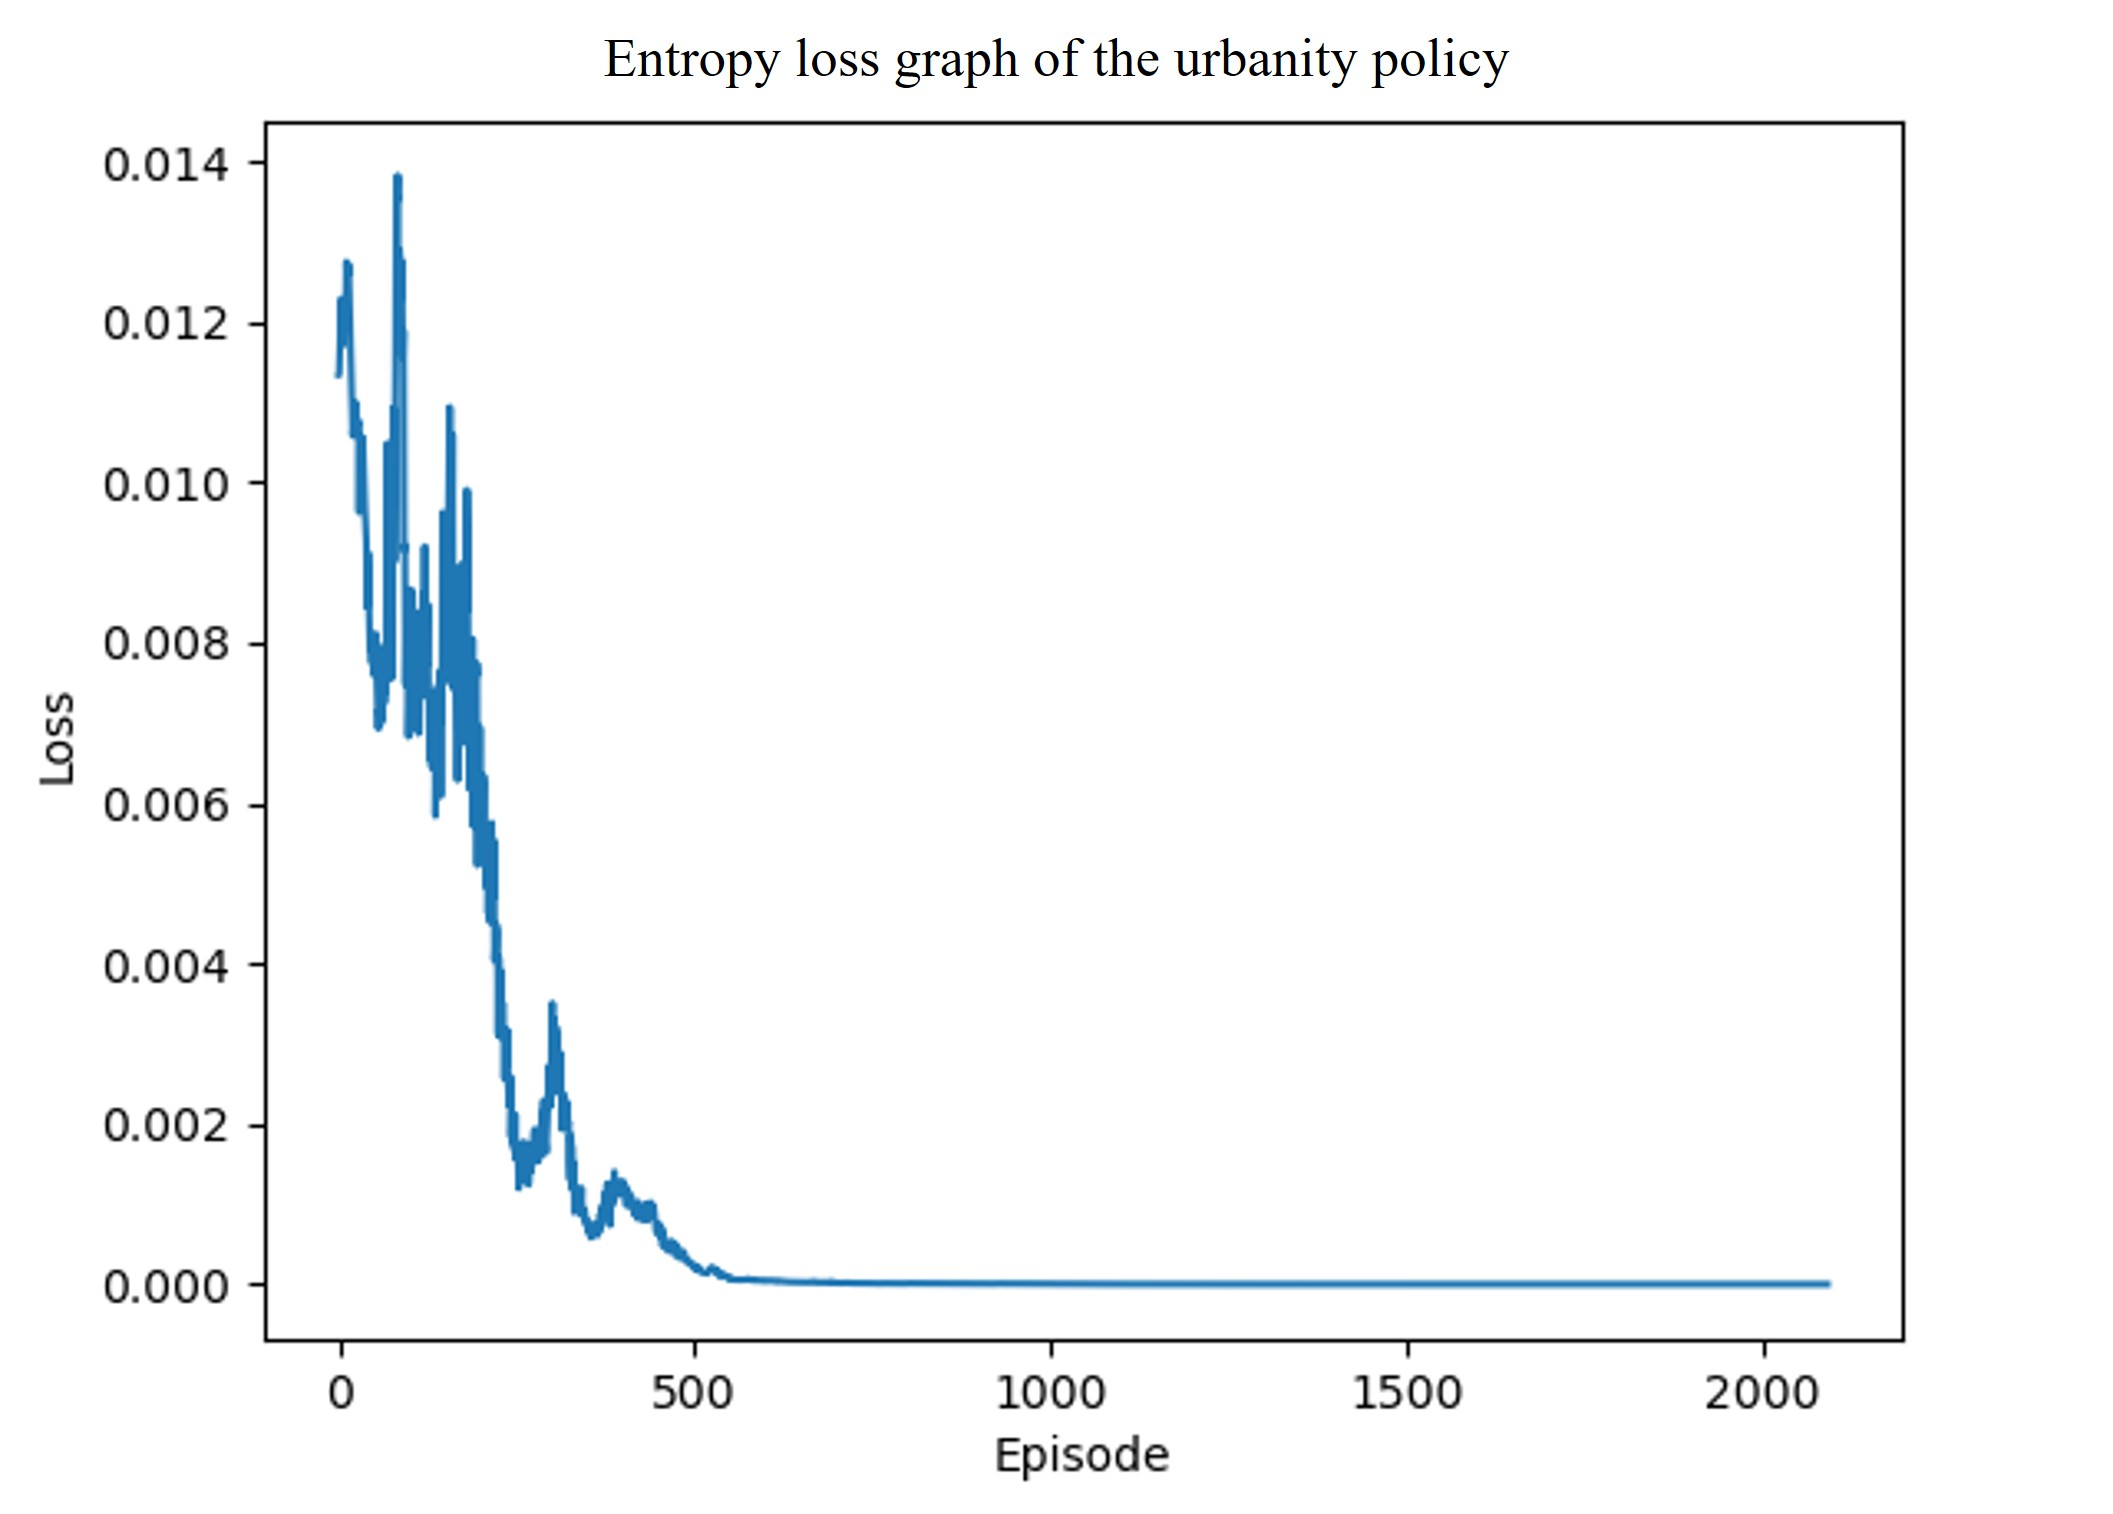
\includegraphics[width=0.7\linewidth]{paper/doc/result_figure/AFMORL_urb_entr_loss_v1.jpg}
    \caption{Entropy loss graph of the urbanity policy}
    
    \label{fig:enter-label}
\end{figure}


%% For citations use: 
%%       \citet{<label>} ==> Lamport [21]
%%       \citep{<label>} ==> [21]
%%

%% If you have bib database file and want bibtex to generate the
%% bibitems, please use
%%
%%  \bibliographystyle{elsarticle-num-names} 
%%  \bibliography{<your bibdatabase>}

%% else use the following coding to input the bibitems directly in the
%% TeX file.

%% Refer following link for more details about bibliography and citations.
%% https://en.wikibooks.org/wiki/LaTeX/Bibliography_Management

\cleardoublepage

\begin{thebibliography}{00}

%% For authoryear reference style
%% \bibitem[Author(year)]{label}
%% Text of bibliographic item
\bibitem{EPA2022}
United States Environmental Protection Agency (EPA). (2022).
Sources of greenhouse gas emissions.
Retrieved from https://www.epa.gov/ghgemissions/sources-greenhouse-gas-emissions/. Accessed May 1, 2025.
\bibitem{Chakr2022}
Chakraborty, P., Parker, R., Hoque, T., Cruz, J., Du, L., Wang, S., \& Bhunia, S. (2022). Addressing the range anxiety of battery electric vehicles with charging en route. \textit{Scientific Reports}, 12(1), 5588. https://doi.org/10.1038/s41598-022-08942-2.
\bibitem{Singh2025}
Singh, D., Singh, S. K., Singh, S., Singh, U., \& Singh, B. (2025, February). Electric Vehicles: Types, Advantages, Difficulties, and Possible Remedies for Broad Adoption: A Review. In \textit{2025 International Conference on Intelligent Control, Computing and Communications (IC3)} (pp. 1324-1328). IEEE. https://doi.org/10.1109/IC363308.2025.10956685.
\bibitem{Li_kha2019}
Li, Z., Khajepour, A., \& Song, J. (2019). A comprehensive review of the key technologies for pure electric vehicles. \textit{Energy}, 182, 824-839. https://doi.org/10.1016/j.energy.2019.06.077. 
\bibitem{Masri2024}
Masri, J., Amer, M., Salman, S., Ismail, M., \& Elsisi, M. (2024). A survey of modern vehicle noise, vibration, and harshness: A state-of-the-art. \textit{Ain Shams Engineering Journal}, 102957. https://doi.org/10.1016/j.asej.2024.102957.
\bibitem{Shi_Hao2021}
Shi, L., Hao, Y., Lv, S., Cipcigan, L., \& Liang, J. (2021). A comprehensive charging network planning scheme for promoting EV charging infrastructure considering the Chicken-Eggs dilemma. \textit{Research in Transportation Economics}, 88, 100837. https://doi.org/10.1016/j.retrec.2020.100837.
\bibitem{Town2022}
Town, G., Taghizadeh, S., \& Deilami, S. (2022). Review of fast charging for electrified transport: demand, technology, systems, and planning. \textit{Energies}, 15(4), 1276. https://doi.org/10.3390/en15041276.
\bibitem{Biroon2019}
Biroon, R. A., Abdollahi, Z., \& Hadidi, R. (2019, September). Fast and regular electric vehicle charging impacts on the distribution feeders. \textit{In 2019 IEEE Industry Applications Society Annual Meeting} (pp. 1-7). IEEE. https://doi.org/10.1109/IAS.2019.8912036. 
\bibitem{Hanig2025}
Hanig, L., Ledna, C., Nock, D., Harper, C. D., Yip, A., Wood, E., \& Spurlock, C. A. (2025). Finding gaps in the national electric vehicle charging station coverage of the United States. \textit{Nature Communications}, 16(1), 561. https://doi.org/10.1038/s41467-024-55696-8.
\bibitem{Roy2022}
Roy, A., \& Law, M. (2022). Examining spatial disparities in electric vehicle charging station placements using machine learning. \textit{Sustainable cities and society}, 83, 103978. https://doi.org/10.1016/j.scs.2022.103978
\bibitem{Sharma2022}
Sharma, S., \& Kumar, V. (2022). A comprehensive review on multi-objective optimization techniques: Past, present and future. \textit{Archives of Computational Methods in Engineering}, 29(7), 5605-5633. https://doi.org/10.1007/s11831-022-09778-9.
\bibitem{Liu_wen2012}
Liu, Z., Wen, F., \& Ledwich, G. (2012). Optimal planning of electric-vehicle charging stations in distribution systems. \textit{IEEE transactions on power delivery}, 28(1), 102-110. https://doi.org/10.1109/TPWRD.2012.2223489.
\bibitem{Zeb2020}
Zeb, M. Z., Imran, K., Khattak, A., Janjua, A. K., Pal, A., Nadeem, M., ... \& Khan, S. (2020). Optimal placement of electric vehicle charging stations in the active distribution network. \textit{IEEE Access}, 8, 68124-68134. https://doi.org/10.1109/ACCESS.2020.2984127.
\bibitem{Kazemt2024}
Kazemtarghi, A., Mallik, A., \& Chen, Y. (2024). Dynamic pricing strategy for electric vehicle charging stations to distribute the congestion and maximize the revenue. \textit{International Journal of Electrical Power \& Energy Systems}, 158, 109946. https://doi.org/10.1016/j.ijepes.2024.109946.
\bibitem{Jordan2022}
Jordán, J., Palanca, J., Martí, P., \& Julian, V. (2022). Electric vehicle charging stations emplacement using genetic algorithms and agent-based simulation. \textit{Expert Systems with Applications}, 197, 116739. https://doi.org/10.1016/j.eswa.2022.116739.
\bibitem{Wang_Tao2022}
Wang, Y., Tao, S., Chen, X., Huang, F., Xu, X., Liu, X., Liu, Y., \& Liu, L. (2022). Method multi-criteria decision-making method for site selection analysis and evaluation of urban integrated energy stations based on geographic information system. \textit{Renewable energy}, 194, 273-292. https://doi.org/10.1016/j.renene.2022.05.087. 
\bibitem{Guo_zhao2015}
Guo, S., \& Zhao, H. (2015). Optimal site selection of electric vehicle charging station by using fuzzy TOPSIS based on sustainability perspective. \textit{Applied Energy}, 158, 390-402. https://doi.org/10.1016/j.apenergy.2015.08.082.
\bibitem{Petratos2021}
Padmanabhan, S., Petratos, A., Ting, A., Zhou, K., Hageman, D., Pisel, J. R., \& Pyrcz, M. J. (2021). Optimal placement of public electric vehicle charging stations using deep reinforcement learning. arXiv preprint arXiv:2108.07772. https://doi.org/10.48550/arXiv.2108.07772.
\bibitem{Ting_Lin2024}
Ting, L. P. Y., Lin, C. C., Lin, S. H., Chu, Y. L., \& Chuang, K. T. (2024, April). Multi-agent Reinforcement Learning for Online Placement of Mobile EV Charging Stations. In Pacific-Asia Conference on Knowledge Discovery and Data Mining (pp. 284-296). \textit{Singapore: Springer Nature Singapore}. https://doi.org/10.1007/978-981-97-2262-4\_23.
\bibitem{Huang_zhou2024}
Huang, J., \& Zhou, X. (2024, April). Optimizing EV Charging Station Placement in New South Wales: A Soft Actor-Critic Reinforcement Learning Approach. \textit{In 2024 5th International Conference on Computer Engineering and Application (ICCEA)} (pp. 1790-1794). IEEE. https://doi.org/10.1109/ICCEA62105.2024.10603658.
\bibitem{Heo2024}
Heo, J., \& Chang, S. (2024). Optimal planning for electric vehicle fast charging stations placements in a city scale using an advantage actor-critic deep reinforcement learning and geospatial analysis. \textit{Sustainable Cities and Society}, 113, 105567. https://doi.org/10.1016/j.scs.2024.105567.
\bibitem{Liu_Xiang2018}
Liu, Y., Xiang, Y., Tan, Y., Wang, B., Liu, J., \& Yang, Z. (2018). Optimal allocation model for EV charging stations coordinating investor and user benefits. \textit{IEEE Access}, 6, 36039-36049. https://doi.org/10.1109/ACCESS.2018.2843810.
\bibitem{zapot2024}
Zapotecas-Martínez, S., Armas, R., \& García-Nájera, A. (2024). A multi-objective evolutionary approach for the electric vehicle charging stations problem. \textit{Expert Systems with Applications}, 240, 122514. https://doi.org/10.1016/j.eswa.2023.122514.
\bibitem{Pourvaziri2024}
Pourvaziri, H., Sarhadi, H., Azad, N., Afshari, H., \& Taghavi, M. (2024). Planning of electric vehicle charging stations: An integrated deep learning and queueing theory approach. \textit{Transportation Research Part E: Logistics and Transportation Review}, 186, 103568. https://doi.org/10.1016/j.tre.2024.103568.
\bibitem{Panah2022}
Panah, P. G., Bornapour, S. M., Nosratabadi, S. M., \& Guerrero, J. M. (2022). Hesitant fuzzy for conflicting criteria in multi-objective deployment of electric vehicle charging stations. \textit{Sustainable Cities and Society}, 85, 104054. https://doi.org/10.1016/j.scs.2022.104054.
\bibitem{Alberti1996}
Alberti, M. (1996). Measuring urban sustainability. \textit{Environmental impact assessment review}, 16(4-6), 381-424. https://doi.org/10.1016/S0195-9255(96)00083-2.
\bibitem{Erbas2018}
Erbaş, M., Kabak, M., Özceylan, E., \& Çetinkaya, C. (2018). Optimal siting of electric vehicle charging stations: A GIS-based fuzzy Multi-Criteria Decision Analysis. \textit{Energy}, 163, 1017-1031. https://doi.org/10.1016/j.energy.2018.08.140.
\bibitem{Hosseini2019}
Hosseini, S., \& Sarder, M. D. (2019). Development of a Bayesian network model for optimal site selection of electric vehicle charging station. \textit{International Journal of Electrical Power \& Energy Systems}, 105, 110-122. https://doi.org/10.1016/j.ijepes.2018.08.011.
\bibitem{kaya_alemdar2022}
Kaya, Ö., Alemdar, K. D., Atalay, A., Çodur, M. Y., \& Tortum, A. (2022). Electric car sharing stations site selection from the perspective of sustainability: A GIS-based multi-criteria decision making approach. \textit{Sustainable Energy Technologies and Assessments}, 52, 102026. https://doi.org/10.1016/j.seta.2022.102026.
\bibitem{Ghosh2021}
Ghosh, A., Ghorui, N., Mondal, S. P., Kumari, S., Mondal, B. K., Das, A., \& Gupta, M. S. (2021). Application of hexagonal fuzzy MCDM methodology for site selection of electric vehicle charging station. \textit{Mathematics}, 9(4), 393. https://doi.org/10.3390/math9040393.
\bibitem{Hisoglu2023}
Hisoglu, S., Tuominen, A., \& Huovila, A. (2023). An approach for selecting optimal locations for electric vehicle solar charging stations. \textit{IET Smart cities}, 5(2), 123-134. https://doi.org/10.1049/smc2.12058.
\bibitem{Kaya_Alem2021}
Kaya, Ö., Alemdar, K. D., Campisi, T., Tortum, A., \& Çodur, M. K. (2021). The development of decarbonisation strategies: a three-step methodology for the suitable analysis of current EVCS locations applied to Istanbul, Turkey. \textit{Energies}, 14(10), 2756. https://doi.org/10.3390/en14102756.
\bibitem{Bi2025}
Bi, H., Gu, Y., Lu, F., \& Mahreen, S. (2025). Site selection of electric vehicle charging station expansion based on GIS-FAHP-MABAC. \textit{Journal of Cleaner Production}, 145557. https://doi.org/10.1016/j.jclepro.2025.145557.
\bibitem{DOE_EVCSL}
U.S. Department of Energy (DOE). (2025). Electric vehicle charging station locations. Retrieved from https://afdc.energy.gov/stations\#/find/nearest/. Accessed May 1, 2025.
\bibitem{Chou2017}
Chou, P. W., Maturana, D., \& Scherer, S. (2017, July). Improving stochastic policy gradients in continuous control with deep reinforcement learning using the beta distribution. \textit{In International conference on machine learning} (pp. 834-843). PMLR. https://proceedings.mlr.press/v70/chou17a.html.
\bibitem{Oliveira2021}
de Oliveira, T. H. F., de Souza Medeiros, L. P., Neto, A. D. D., \& Melo, J. D. (2021). Q-Managed: A new algorithm for a multiobjective reinforcement learning. \textit{Expert Systems with Applications}, 168, 114228. https://doi.org/10.1016/j.eswa.2020.114228.
\bibitem{Hayes2022}
Hayes, C. F., Rădulescu, R., Bargiacchi, E., Källström, J., Macfarlane, M., Reymond, M., Verstraeten, T., Zintgraf, L. M., Dazeley, R., Heintz, F., \& Howley, E. (2022). A practical guide to multi-objective reinforcement learning and planning. \textit{Autonomous Agents and Multi-Agent Systems}, 36(1), 26. https://doi.org/10.1007/s10458-022-09552-y.
\bibitem{Carlton2022}
Carlton, G. J., \& Sultana, S. (2022). Electric vehicle charging station accessibility and land use clustering: A case study of the Chicago region. \textit{Journal of Urban Mobility}, 2, 100019. https://doi.org/10.1016/j.urbmob.2022.100019.
\bibitem{Bhargava2024}
Bhargava, R., Zhang, R., \& Kontou, E. (2024). Heterogeneity of Land Uses near Electric Vehicle Charging Stations and their Affordability in Chicago, Illinois. \textit{Findings}. https://doi.org/10.32866/001c.125835.
\end{thebibliography}

\end{document}

\endinput
%%
%% End of file `elsarticle-template-num-names.tex'.
